\documentclass[10pt]{article} % Font size - 10pt, 11pt or 12pt

\usepackage[hmargin=1.25cm, vmargin=1.5cm]{geometry} % Document margins
\usepackage[usenames,dvipsnames]{xcolor} % Allows the definition of hex colors

\usepackage{listings}
\lstset{escapechar=\&}

% Fonts and tweaks for XeLaTeX
\usepackage{fontspec,xltxtra,xunicode}
\defaultfontfeatures{Mapping=tex-text}
%\setmonofont[Scale=MatchLowercase]{Andale Mono}

% Colors for links, text and headings
\usepackage{hyperref}
\definecolor{linkcolor}{HTML}{506266} % Blue-gray color for links
\definecolor{shade}{HTML}{F5DD9D} % Peach color for the contact information box
\definecolor{text1}{HTML}{2b2b2b} % Main document font color, off-black
\definecolor{headings}{HTML}{701112} % Dark red color for headings
% Other color palettes: shade=B9D7D9 and linkcolor=A40000; shade=D4D7FE and linkcolor=FF0080

\hypersetup{colorlinks,breaklinks, urlcolor=linkcolor, linkcolor=linkcolor} % Set up links and colors

\usepackage{titlesec}
\setcounter{secnumdepth}{4}

\setlength{\emergencystretch}{3cm} % somehow helps prevent hboxes from overflowing

\titleformat{\paragraph}
{\normalfont\normalsize\bfseries}{\theparagraph}{1em}{}
\titlespacing*{\paragraph}
{0pt}{3.25ex plus 1ex minus .2ex}{1.5ex plus .2ex}

\usepackage{fancyhdr}
\usepackage{amssymb}
\usepackage{amsmath}
\pagestyle{fancy}
\fancyhf{}

\usepackage{csquotes}

\usepackage{float}

\renewcommand{\headrulewidth}{0pt} % Get rid of the default rule in the header

\bibliographystyle{plain}

\begin{document}

\tableofcontents
\listoffigures
\newpage

\section{Chapter: Introduction}
\blockquote{An embryo in its spherical blastula stage has spherical symmetry [...]. But a system which has spherical symmetry, and whose state is changing because of chemical reactions and diffusion, will remain spherically symmetrical for ever [...]. It certainly cannot result in an organism such as a horse, which is not spherically symmetrical. \textbf{Alan Turing, The Chemical Basis of Morphogenesis, 1952}}

Cells need to create asymmetric, heterogeneous structures inside themselves in order to function. However, as per the above quote, diffusive processes cannot create this asymmetry. How then do cells create heterogeneity? Motor proteins are part of the answer. Motor proteins are structures which use energy to create directed motion in cells. In broad terms, they are creators of asymmetry. This thesis will explore a hypothesis on how one such motor protein, Dynein, generates directed motion.\\

%% \subsection{Interest builder}
%% Begin with a paper-like introduction which talks about:

%% \begin{itemize}
%% \item How dynein is a structure which turns chemical energy into motion
%% \item How dynein's variation in step size and directionality suggest a large diffusion component \cite{reck2006single}
%% \item How it's weird that a cellular structure can generate directed motion
%% \item Other cool stuff - make dynein mysterious and cool.
%% \end{itemize}

%% Tell a story about dynein! Present the project as a story -- we don't have knowledge abotu dynein, it's really weird, we want to get info about it

\subsection{Interest builder}
Motor proteins are cellular structures which use chemical energy to do work and generate motion. Kinesin, myosin and dynein are the three main motor proteins in cells. Though these proteins have significantly different ancestors [cite], they all evolved into a single similar structure. In biology when a structure is evolved three separate times, it is a sign that nature has found an efficient way for solving a problem. How, then, do motor proteins work?\\

The basic form is simple. Kinesin, myosin and dynein each use two binding domains to attach to a surface. These binding domains are connected via a linker domain. Each motor protein is an engine which undergoes cycles, where each cycle moves the motor across a surface. In a single cycle a binding domain will unbind from a surface, tense its foot to kick forward, rebind, then untense its foot to pull the whole motor forward. This pattern is repeated by both feet to generate motion \cite{kinesin-cycle} \cite{myosin-cycle}.\\

Although the three motor protein families operate using the same stepping cycle, their behavior differs significantly. Kinesin and myosin are predictable motors which step in the forwards direction with a regular step size [get kinesin, myosin stepping papers]. In contrast, dynein's stepping pattern varies wildly in both size and direction. The motor steps forward on average, but takes steps backwards and to the side quite regularly \cite{weihongpaper}. How can motors which implement the same release, lever, bind, lurch stepping mechanism behave so differently?\\

One possibility is that dynein's size and organization are responsible for the motor's odd stepping pattern. Dynein is much larger than kinesin or myosin, meaning its feet may need to move significantly further over each cycle. Due to the random nature of Brownian motion from water particle collisions, there may be significantly more variance in the path taken by dynein's feet compared to other motor feet. This could explain the large variance in step size. Another contributing factor could be that dynein is so large that it can twist and contort during its step, allowing varying and even backwards steps, which a small motor would be too tense to achieve.\\

This thesis describes an experiment which aims to test whether Brownian motion and flexibility are what give rise to dynein's unique stepping pattern. To do this, a mathematical model of a dynein-like motor is constructed which exhibits flexibility and feels Brownian forces. This model is then simulated, and its behavior is compared to the behavior of real dynein.\\

%% Dynein:
%% feet which bind to track
%% motor connected to feet which generates the force
%% -----------
%% ATP binding causes dissociation
%% Also causes forward kick
%% ATP hydrolysis
%% rebinding causes ADP rejection and forward lurch
%% restart

%% Kinesin:
%% feet which bind to track
%% connected via lever arm to cargo binding domain
%% -----------
%% ATP binding causes forward kick
%% ATP hydrolysis
%% MT binding, ADP, Pi rejection
%% Other foot unbinds

%% Myosin:
%% Feet which bind to track
%% connected via lever arm to cargo binding domain
%% ----------
%% actin binding causes Pi rejection, strengthening binding
%% binding causes foot to change relative to lever, shifting the motor forward
%% ATP binding causes dissocaition and undoing the powerstroke

\subsection{What is dynein?}
\subsubsection{Basics}
Dynein is a cellular structure which converts chemical energy to mechanical energy. It does so by reacting with adenosine triphosphate (ATP) to take steps along long cellular tracks known as microtubules (MTs). Dynein's mechanical energy is used for various cellular functions, including to transport molecules around the cell, pull chromosomes during division, and move cellular propellers known as cilia \cite{cianfroccoreview}.\\

Dynein is a protein with many smaller domains. A depiction of the protein and its labeled subdomains is shown in Figure (\ref{dynein-artist-rendition}). Each motor is a homodimer made up of two identical monomer proteins. Each monomer has a binding domain which binds to the microtubule, a motor domain which binds ATP, a tail domain which connects to the other monomer, a stalk which connects the binding and motor domains, and a linker which connects the motor and tail domains. The tail domain is also responsible for binding to cargo.\\

\begin{figure}[h]
  \centering
  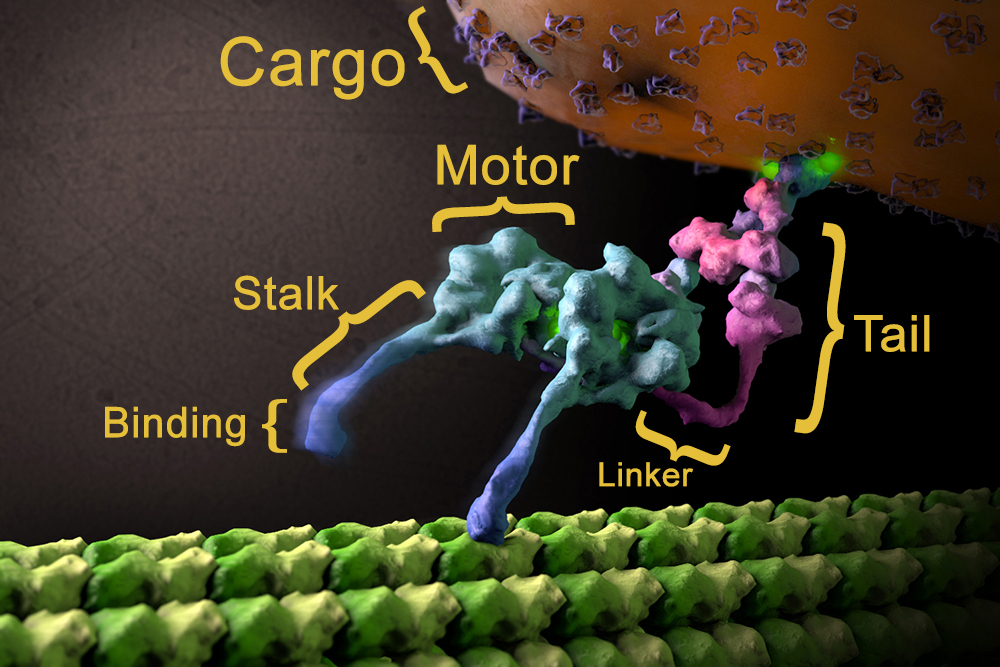
\includegraphics[width=.65\textwidth,keepaspectratio]{../../figures/dynein-artist-rendition.jpg}
  \caption{Artist's rendition of dynein bound to a microtubule.}{One monomer is bound to the MT, and the other is raised up. Modified. Source: Lander Lab, The Scripps Research Institute.}
  \label{dynein-artist-rendition}
\end{figure}

Dynein is believed to move by using the energy of ATP to cycle through a ring of states, each with different spatial relations to the microtubule. By cycling forward through this ring, the molecule will end up in the same state it began, but moved forward a small amount. This ring of states is known as the mechanochemical cycle \cite{cianfroccoreview}. The goal of this project is to create a mathematical model of the mechanochemical cycle and verify that it can reproduce experimental dynein stepping data. There are several types of dynein which all behave differently. This project will focus on cytoplasmic dynein-1, hereby referred to as dynein.\\

\subsubsection{Why do cells need motor transport?}
Cells are organized, heretogenous structures which respond quickly to their environments. This means that cells require a mechanism for rapidly moving components to precise locations within the cell. This can be a challenge, since cells are fairly large compared to the proteins which compose them. A human fibroblast cell has a volume of roughly 2000 $\mu m^3$\cite{fibroblastvolume}, corresponding to roughly $8 \mu m$ in diameter. In comparison, human hemoglobin has a diameter of roughly $5 nm$ (PDB id 5ME2), a $10^3$ factor difference in size.\\

Diffusion, or random motion of molecules due to collisions with solvent (i.e. Brownian motion), is one possible process cells could use to transport biomolecules. Diffusion has two problems: it is slow and nondirected. The expected distance covered for one-dimensional Brownian motion after time t was found by Einstein to be \cite{einstein-paper}:

\begin{equation}
  \label{diffusion-equation}
  <x> = \sqrt{2Dt}
\end{equation}

where D is the diffusion constant describing the diffusability of the biomolecule. For a medium-sized (140kD, 1D = weight of H atom) protein with a diffusion constant $D = .2 \mu m^2/s$ \cite{diffusionconstants}, it would take about a month to travel across a millimeter-sized cell. In contrast, it would take dynein, which travels at roughly 100nm/s \cite{weihongpaper}, a much more reasonable three hours to do the same. Figure (\ref{fig:diffusion_vs_dynein}) demonstrates how motor transport quickly outstrips diffusion in a cell.\\

\begin{figure}[h]
  \centering
  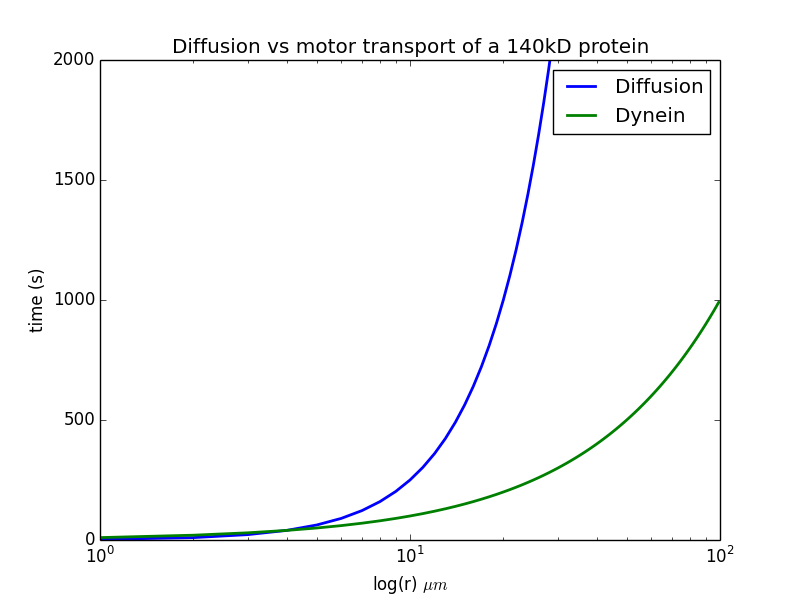
\includegraphics[width=.65\textwidth,keepaspectratio]{../../figures/diffusion_vs_dynein.png}
  \caption{Passive diffusion vs motor transport rate}{Plot comparing the diffusion rate of a 140kD protein with a diffusion consant $D = .2 \mu m^2/s$ with a dynein motor travelling at 100nm/s.}
  \label{fig:diffusion_vs_dynein}
\end{figure}

\textit{Maybe use the more reasonable 2$\mu m / s$ number for dynein velocity, in-vitro speed may not be applicable since [ATP]-limited}

Another advantage of motor transport is that microtubules can be highly specific in their location in the cell. During cell division chromosomes line up at the center of each cell in a plane. Such a geometrically precise shape requires some sort of directed motion which a random process could never provide.\\

\textit{maybe decorate the above plot with pictures of cells of each size, or how long certain cellular events take? That could be cool and make it actually an interesting plot}
\textit{this argument would be much better if you could find examples of things which need to be done quickly in the cell, like responding to foreign particles or signalling molecules or cell division or neural events}

\subsubsection{What role does dynein play in the cell?}
Some of dynein's primary roles in the cell are to transport cellular cargos such as organelles, vesicles, mRNA, cytoskeletal filaments and certain proteins. Dynein also plays a role in positioning and breaking down the nucleus, cell death, spindle formation and the placement of other important cellular structures \cite{valetoolbox}.\\

Microtubules are long polymers of alternating $\alpha-$ and $\beta-$ tubulin subunits. MTs are polar, meaning they have a distinct directionality based on the orientation of thetubulin proteins which comprise them. One pole, the minus end, is where they initiate formation, typically at a MTOC (microtubule organizing center) around the center of the cell. The other pole, the plus end, is where they grow and shrink from. Kinesin and myosin, two other families of motor protein, typically walk towards the plus end of the MT. Dynein is unique in that it walks towards the minus end, making it a minus end-directed motor. This lends it to a particularly important function inside neurons known as retrograde transport.\\

Neurons have cell bodies at their centers and axons which grow outwards. Axons are long, narrow structures extending up to a meter in length in humans. Cell bodies contain nuclei and important organelles for synthesizing proteins, but growth of axon tips is vital for neuron function. This means bidirectional motor transport between axon tips and cell bodies is very important in neurons, since diffusion would not be quick enough. Retrograde transport is transport from the axon tip to the cell body. Cargo includes vesicles full of proteins ready to be broken down in the cell body and microtubule fragments to be returned from the axon tip \cite{neuroanatomy}. Because microtubule minus ends are found in the cell body, dynein's minus end-directed nature makes it the only protein capable of retrograde transport. An interesting question is, if proteins like dynein are synthesized in the cell body but needed at the axon tip to perform retrograde transport, how do dynein get to the tip? The answer is shown in \ref{retrograde-transport}: kinesin, a plus end-directed motor, takes dynein to the tip from the cell body.\\

\begin{figure}[h]
  \centering
  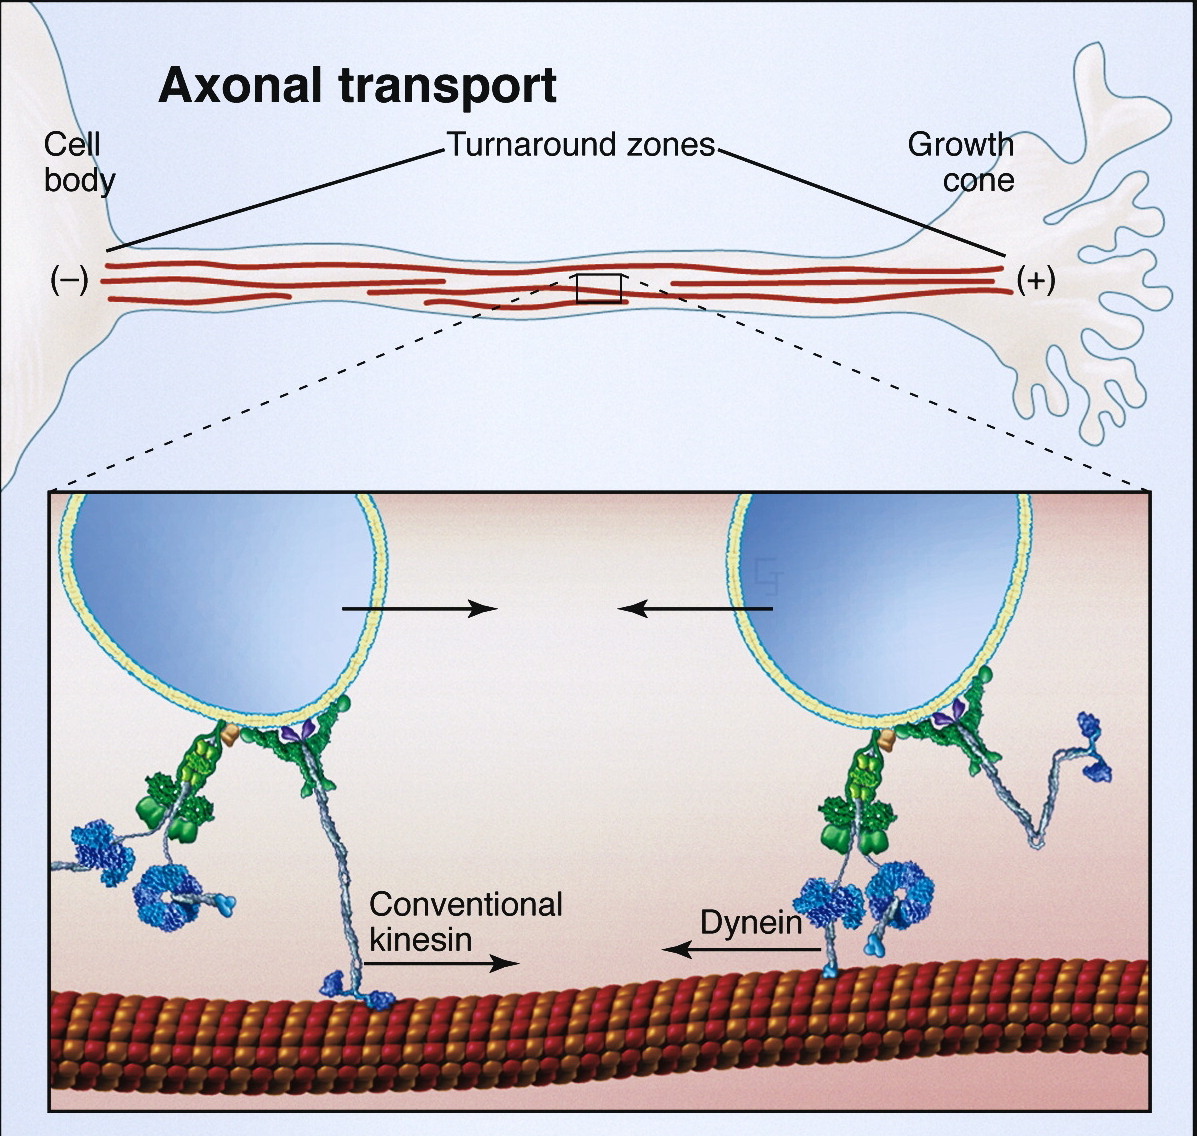
\includegraphics[width=.65\textwidth,keepaspectratio]{../../figures/retrograde_transport.jpg}
  \caption{Dynein localization to axon growth cones.}{Mechanism of dynein localization to axon tips, or growth cones, in retrograde transport mediated by kinesin anterograde transport. Modified from \cite{valetoolbox}.}
  \label{retrograde-transport}
\end{figure}

\subsubsection{Dynein structure}

\begin{figure}[h]
  \centering
  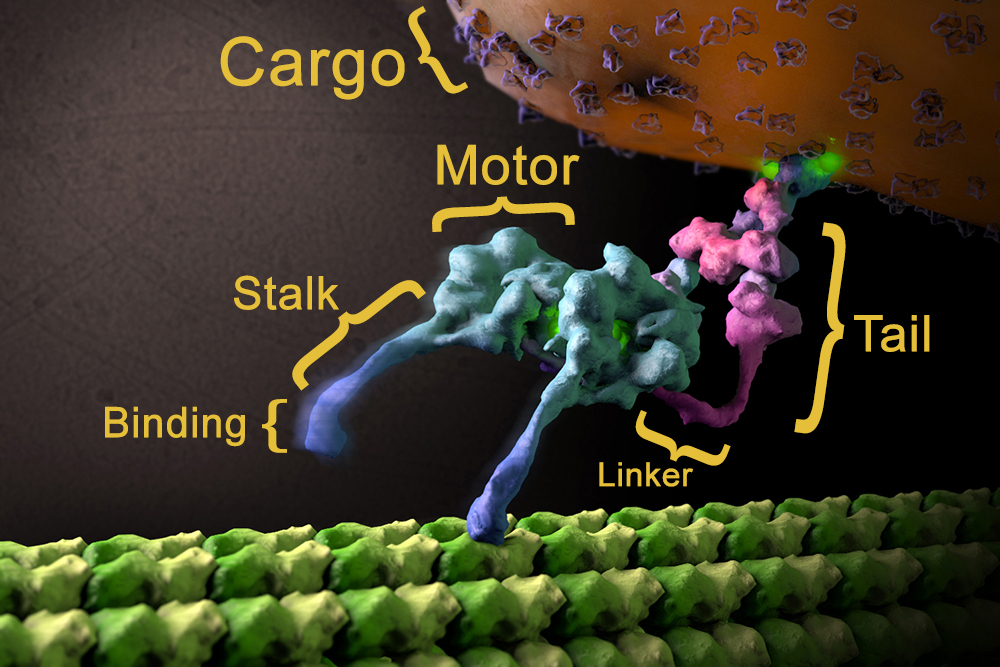
\includegraphics[width=.65\textwidth,keepaspectratio]{../../figures/dynein-artist-rendition.jpg}
  \caption{Artist's rendition of motor-MT complex.}{Artist rendition of the dynein motor bound to a microtubule. One monomer is bound to the MT, and one is raised up. Modified. Source: Lander Lab, The Scripps Research Institute.}
  \label{dynein-artist-rendition-2}
\end{figure}

\textit{eventually find a different figure}

As shown in \ref{dynein-artist-rendition-2}, a dynein motor is a fusion of two identical subunits, or monomers, each with binding, stalk, motor and tail subdomains. Each of these subunits has a unique purpose for the motor.

\textbf{Binding domain}
Microtubule binding domains (MTBDs) allow dynein to bind to the microtubule. 

%% \begin{figure}[h]
%%   \centering
%%   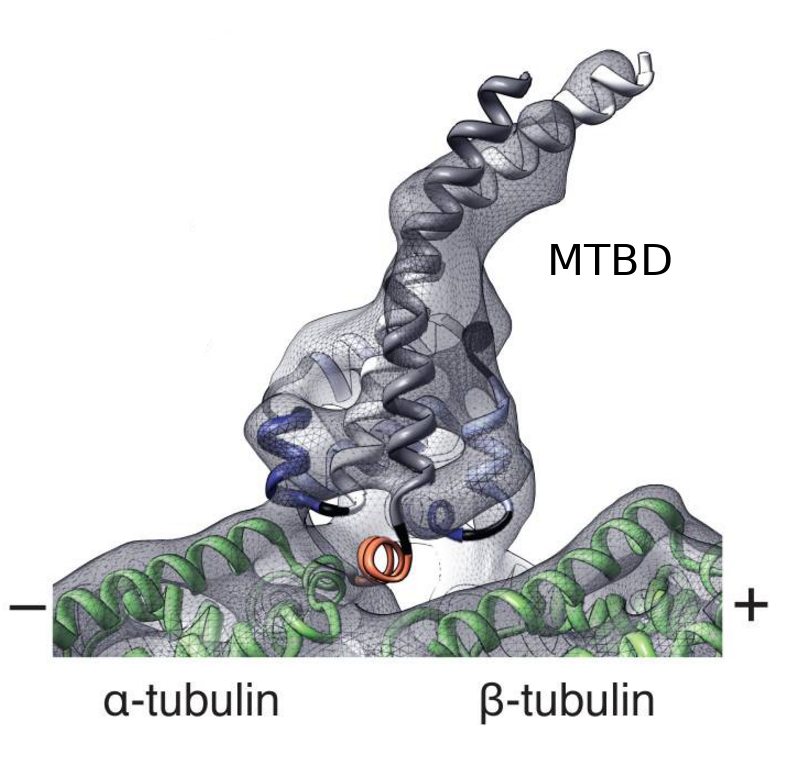
\includegraphics[width=.65\textwidth,keepaspectratio]{../../figures/mtbd-complex.png}
%%   \caption{Crystal structure of the MTBD-MT complex. Modified from Redwine \textit{et. al} \cite{redwineMTBDcomplex}.}
%%   \label{dynein-artist-rendition-2}
%% \end{figure}

\subsubsection{How does it behave?}
Talk about its stepping behavior using Weihong's figures (as well as the new paper David found?)\\

Also possibly talk about the other things Dynein has been found to do, such as hydrolyse ATP and move its subdomains around. This may be better in a different section than the introduction though, since its a lot of biochemistry for the second section in an intro? maybe not, it has to go somewhere.

\subsubsection{Why is dynein special and interesting?}
Compare the processive motion of dynein to kinesin in \textbf{a.)} directionality, \textbf{b.)} stepping pattern and \textbf{c.)} size (like how it can step over roadblocks kinesin cannot).\\

Talk about why a random stepping motor is interesting compared to a orderly-stepping motor: what is different about dynein's structure that makes it step differently? Compare the crystal structures and ask lots of questions. Build interest in the motors here.\\

%% \begin{figure}[h]
%%   \centering
%%   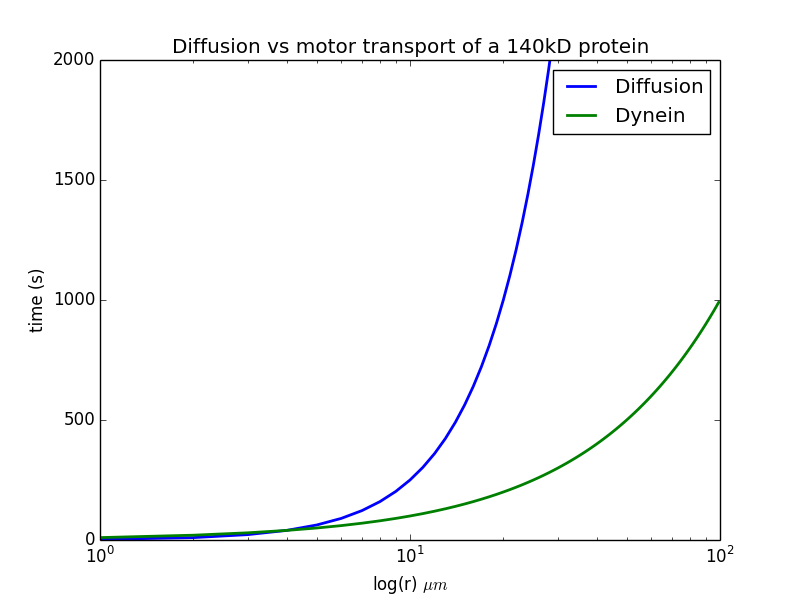
\includegraphics[width=.65\textwidth,keepaspectratio]{../../figures/diffusion_vs_dynein.png}
%%   \caption{Crystal structures of cytoplasmic dynein 1 and kinesin KIF5B (PDB IDs 4RH7 and 1BG2).}
%%   \label{kin_n_dyn}
%% \end{figure}

\textit{make this figure good -- find a full length kinesin crystal structure, not 1BG2. Use kindyn.pse as a template.}

\subsection{Dynein Stepping Background}
Biophysicists and molecular biologists have conducted experiments over the past twenty years which shed light on how the dynein motor might walk. The full mechanism is not known, but results of such experiments suggest a certain vague picture of how dynein generates motion.\\

\subsubsection{ATP cycle influences conformational state}
Dynein is known to occupy multiple discrete conformational states depending on its environment. In particular, the concentration of ATP and microtubules is known to alter the shape dynein takes on. A FRET (fluorescence resonance energy transfer) study attached fluorophores to dynein's motor and tail and measured the average distance between the two \cite{FRETstatepaper}. It was found that average distance increased or decreased depending on the nucleotide bound to dynein, indicating the motor takes on different conformations for different bound nucleotides. Dynein unbound to nucleotide, or frozen in ATP or ADP-bound states, had a similar tail-motor distance. However, when the motor was stuck in an ADP-Pi state, with ATP hydrolyzed but phosphate not yet released, the tail-motor distance was increased. This suggests that dynein starts its cycle with no nucleotide, binds ATP, hydrolyzes ATP, enters the ADP-Pi state and changes conformation to a far tail-motor distance, then releases phosphate, moves back to its original close tail-motor conformation, then ejects ADP and starts over.\\

Studies suggest that near/far tail-motor conformation changes are not due to lengthening of the stem linking the two domains, but rather a change in position of the head relative to the trail \cite{FRETstatepaper} \cite{burgess-paper}. Cryo-electron microscopy images of the dynein motor shown in Figure (\ref{fig:cryo-em-angles}) demonstrate the differences in conformation in the nucleotide-free and ADP-Pi state.\\

\begin{figure}[h]
  \centering
  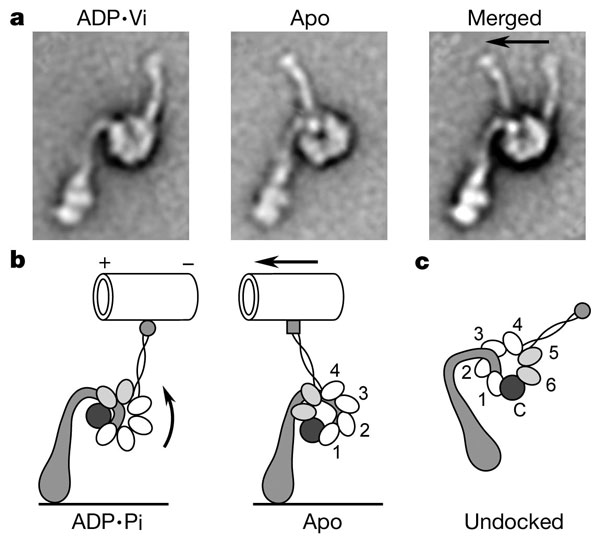
\includegraphics[width=.65\textwidth,keepaspectratio]{../../figures//burgess-dynein-angles}
  \caption{Cryo-EM microscopy of dynein conformational states.}{Cryo-electron microscopy images of dynein in two different nucleotide states. Left: dynein frozen in ADP-Pi state. Middle: dynein without nucleotide. Right: two states superimposed on one another. Bottom: cartoons representing how dynein may bind to the MT in either state. From \cite{burgess-paper}.}
  \label{fig:cryo-em-angles}
\end{figure}

Crystal structures of cytoplasmic dynein-2, a relative of dynein, indicate that ATP-Pi binding to the motor domain induces a conformation change in the motor domain, which alters the angle at which the motor binds to the tail \cite{carter-paper} (make a Chimaera figure where the pre/poststroke motors are docked showing this). Taken together, these results indicate that as the motor binds and hydrolyzes ATP, it undergoes a conformation change which physically moves the motor relative to the tail.\\

\textbf{TODO: look at \cite{nicastro} and \cite{schmidt-carter} to see if they can add to this discussion}

\subsubsection{Microtubule and nucleotide states are coupled}
Dynein is known to bind to the microtubule at a location known as the $\alpha$-$\beta$ polymerization site \cite{redwineMTBDcomplex}. This site occurs roughly every 8nm, indicating dynein is restricted to step sizes which are multiples of 8nm.\\

The nucleotide state of the motor is not the only determiner of dynein conformation; microtubule binding state has also been shown to influence conformation. A study on the MTBD-MT complex indicates the stalk connecting the motor and MTBD can take on two major conformations, depending on whether the MTBD is bound to the MT or not \cite{mt-atp-coupling}. The conformation of the stalk has been shown to communicate information between the motor and MTBD. In the presence of microtubules, the ATPase rate of the motor is increased 25-fold. This indicates the stalk communicates MT-binding state of the MTBD to the motor, increasing its ATP hydrolysis rate. The communication happens the other way, as well. Treating dynein with ATP causes MT-binding rate to drop 15-fold, indicating ATP-binding at the motor decreases MT-binding rate at the MTBD.\\

In addition to a bidirectional linking between ATPase rate and MT-binding, stalk state has been shown to directly influence motor conformation \cite{mt-atp-coupling}. When the stalk is allowed to freely transition between bound and unbound states, the motor can also transition between near and far tail/motor states. However, when the stalk is frozen in a particular conformation, the motor loses its transitioning ability. This suggests that the conformations of the two systems are tightly linked.\\

\subsubsection{Stepping pattern}
Several studies have been done on the dynein motor's stepping pattern using selectively-labeled motor domains \cite{reck2006single} \cite{weihongpaper}. These studies show dynein's stepping pattern to be stochastic and weakly forward-directed. As shown in Figure (\ref{fig:weihong-steps}), dynein takes many backwards steps, and also many steps with components perpendicular to the microtubule. This indicates the process dynein uses to generate motion has a stochastic component to it. It is likely that the physical states of subcomponents in the motor, and/or the effects of Brownian motion due to water particle collision, play a role in dynein's stepping mechanism.\\

\begin{figure}[h!]
  \centering
  \begin{minipage}[b]{0.45\textwidth}
    \includegraphics[width=\textwidth]{../../figures/weihong-step-size}
    \caption{Experimental dynein step size histogram.}{Size of steps taken by dynein motor parallel to microtubule. Positive axis corresponds to steps towards the microtubule minus-end. Figure modified from \cite{weihongpaper}.}
  \end{minipage}
  \hspace{.2cm}
  \begin{minipage}[b]{0.45\textwidth}
    \includegraphics[width=\textwidth]{../../figures/weihong-off-axis-steps}
    \caption{Dynein experimental off-axis stepping size.}{Size of ``off-axis'' steps taken by the dynein motor perpendicular to the microtubule. Figure modified from \cite{weihongpaper}.}
  \end{minipage}
  \label{fig:weihong-steps}
\end{figure}

\subsection{Dynein models}
Data presented in the previous sections paints a picture of dynein as a collection of interconnected parts, each cycling through its own collection of states and influencing other parts. Somehow the protein itneracts with nucleotides and microtubules in a way that allows it to reliably move through the cell. Models presented below take these facts and string them together into cohesive cycles which might explain how dynein walks. It is important to note that these models are hypotheses.\\

\subsubsection{Cianfrocco Model}
Cianfrocco \textit{et. al} \cite{cianfroccoreview} propose dynein achieves motion via transitioning through the cycle of states shown in Fig. \ref{mech-cycle}. This model will hereon be referred to as the Cianfrocco model. The model claims the primary events in the dynein step are as follows. First, starting with both binding domains attached to the MT, ATP binds to the motor domain, which causes it to change conformation. ATP hydrolysis to ADP-Pi causes further conformation changes. These changes cause the binding domain to release the microtubule, meaning only one binding domain is MT-bound. The free binding domain then undergoes another conformation change known as the ``priming stroke,'' which changes the orientation of the binding domain with respect to the MT. Finally the binding domain rebinds to the MT, causing a final conformation change in the motor which returns it to the beginning of the cycle. The exact order of these events is not precisely known.\\

\begin{figure}[h!]
  \centering
  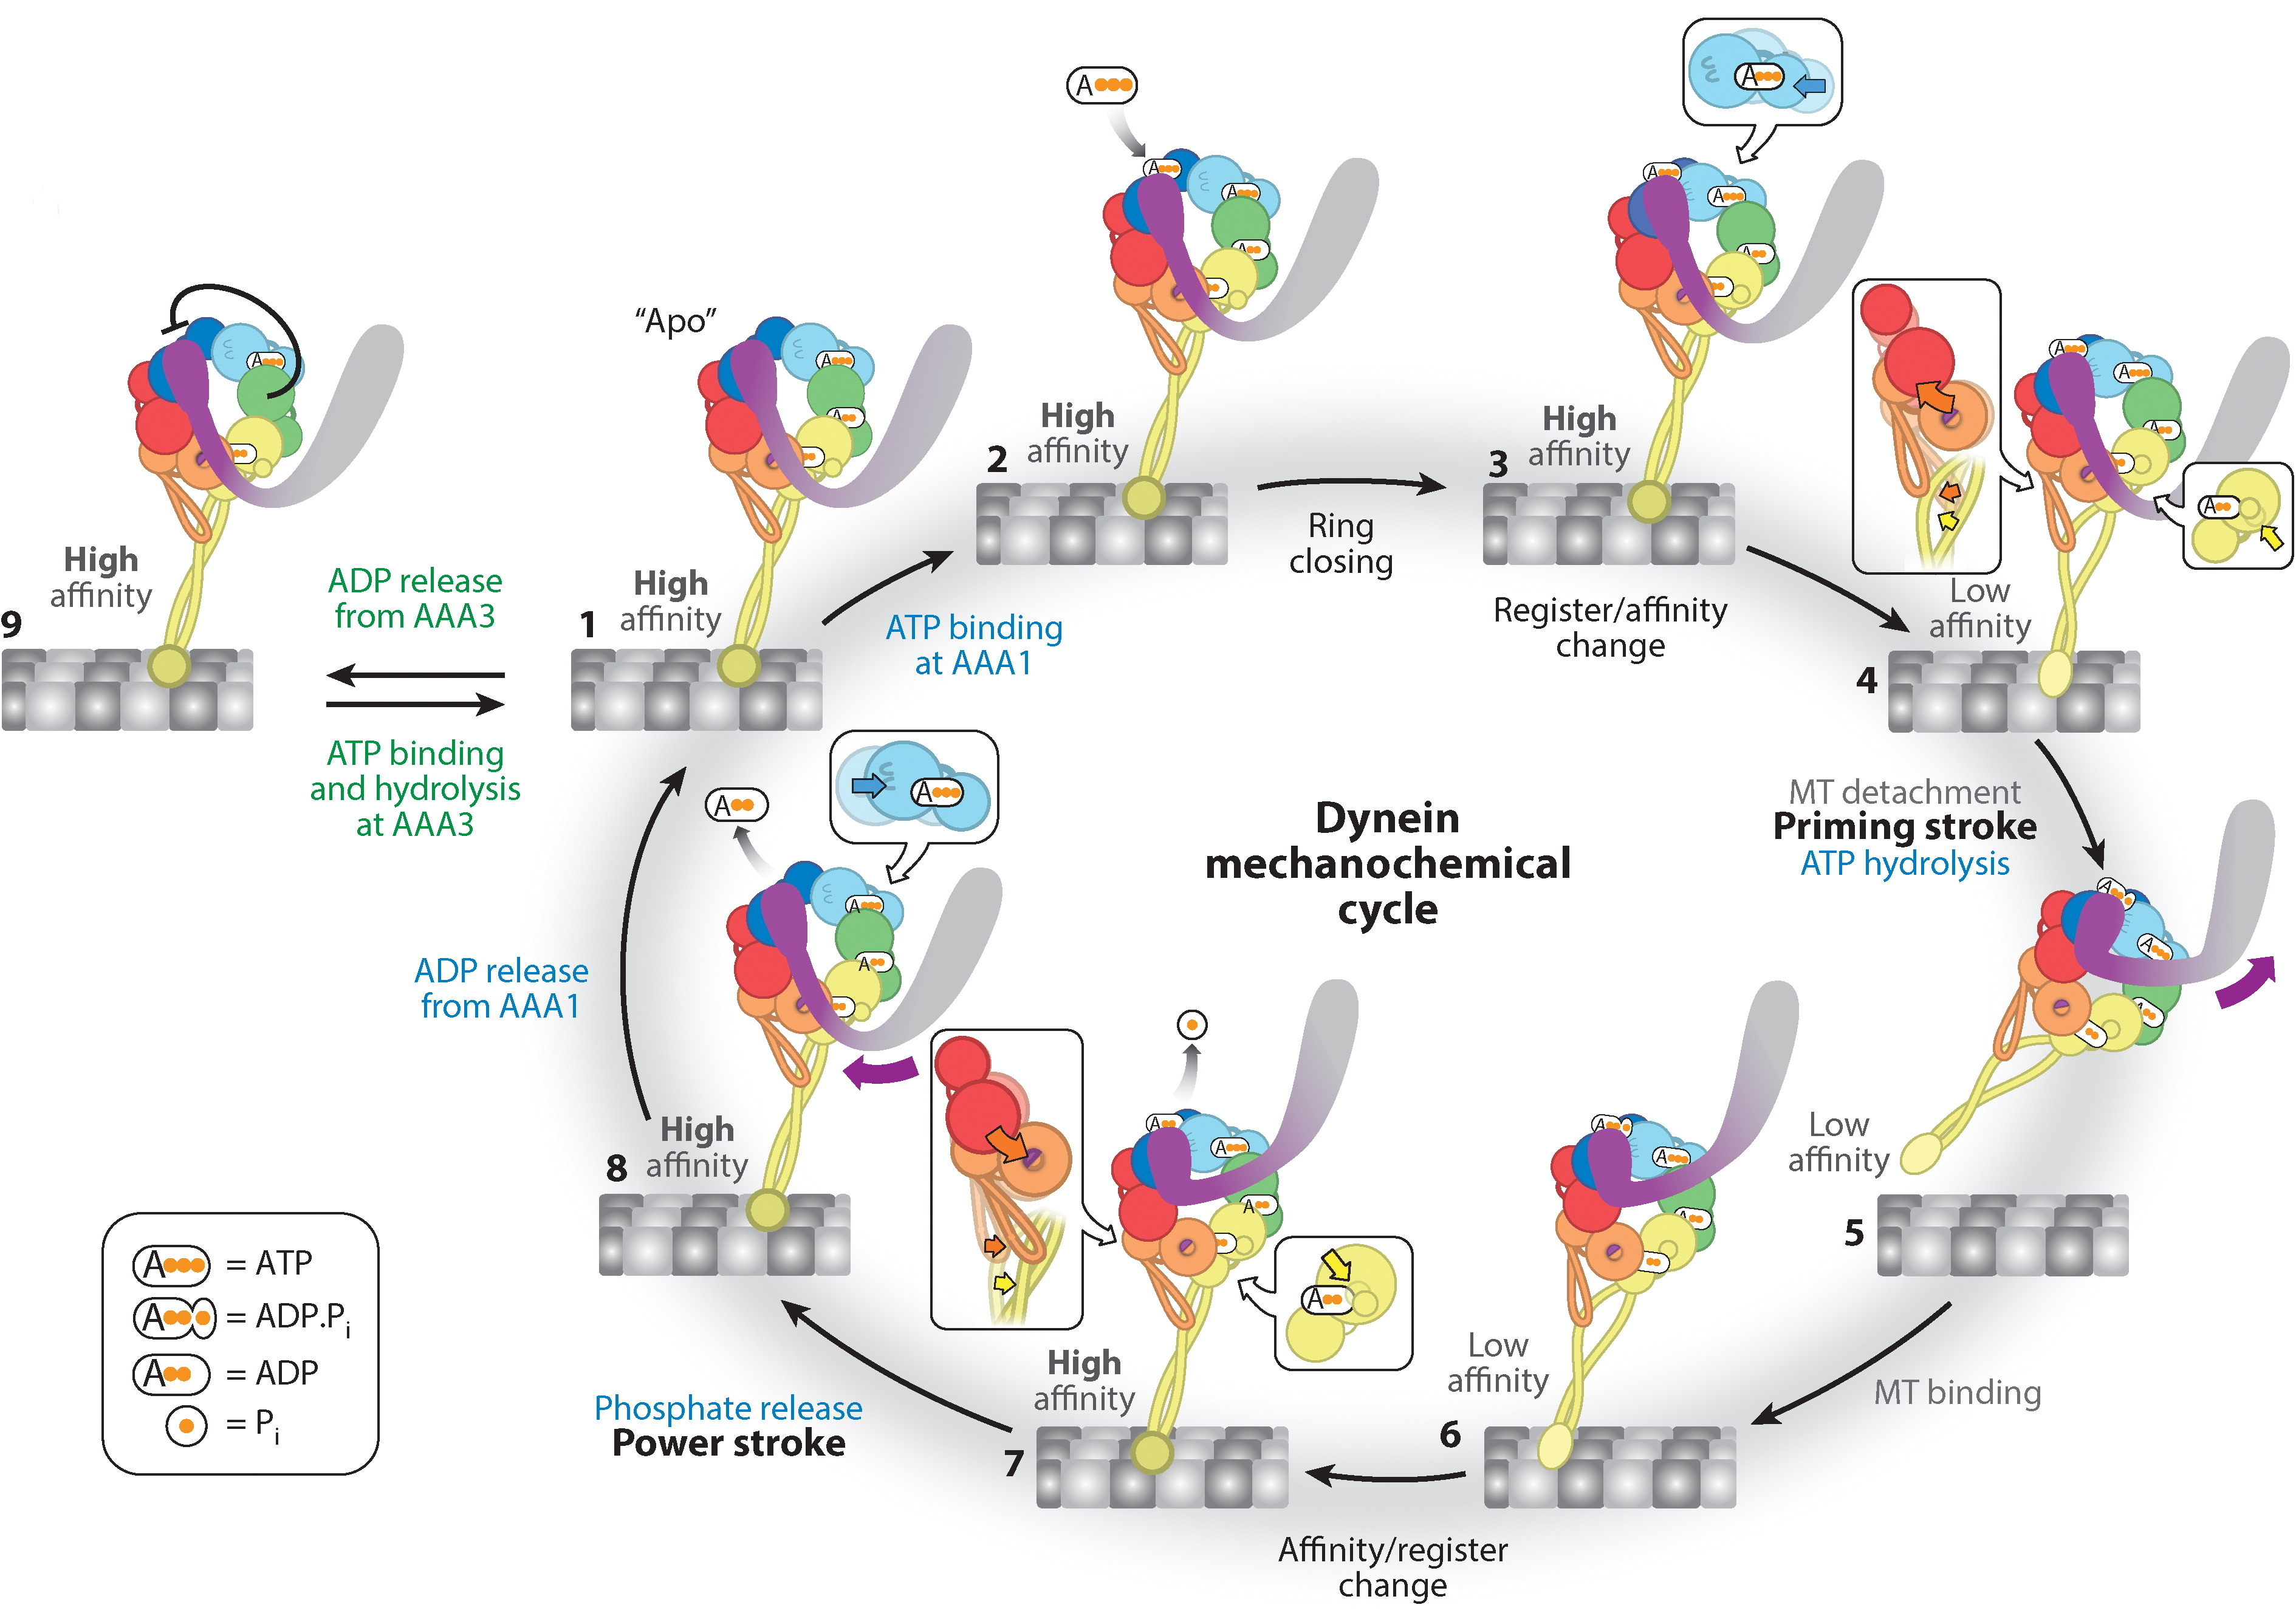
\includegraphics[width=.90\textwidth,keepaspectratio]{../../figures/mechanochemical-cycle.jpeg}
  \newcommand\bothbound{\textcolor{blue}{BOTHBOUND}}
  \newcommand\onebound{\textcolor{red}{ONEBOUND}}
  \newcommand\transition{\textcolor{green}{transition?}}
  %% \begin{tabular}{rll}
  %%   \bothbound &
  %%   1 & \begin{minipage}{5in}
  %%     Bound to microtubule and waiting for ATP to arrive.  The
  %%     conformation is ``post-powerstroke''.
  %%   \end{minipage}\vspace{0.5em}\\
  %%   \bothbound &
  %%   2 & \begin{minipage}{5in}
  %%     ATP has bound to the motor at AAA1, but nothing else has changed.
  %%   \end{minipage}\vspace{0.5em}\\
  %%   \transition &
  %%   3 & \begin{minipage}{5in}
  %%     ``The ring has closed'' in the motor, whatever that means.
  %%   \end{minipage}\vspace{0.5em}\\
  %%   \bothbound &
  %%   4 & \begin{minipage}{5in}
  %%     The affinity to the microtubule is dropped, so it is likely to pop off soon.
  %%   \end{minipage}\vspace{0.5em}\\
  %%   \onebound &
  %%   5 & \begin{minipage}{5in} It has popped off of the microtubule!
  %%     Onebound! The equilibrium angle is also changed.  The ATP has
  %%     been hydrolized, but the phosphate is still bound to the motor.
  %%     ``Priming stroke?''
  %%   \end{minipage}\vspace{0.5em}\\
  %%   \onebound &
  %%   6 & \begin{minipage}{5in} It is now bound to the microtubule, but
  %%     with low affinity, and without any loss of phosphate. Question:
  %%     does this happen many times? If so it may still be onebound.
  %%     Otherwise it is probably bothbound.
  %%   \end{minipage}\vspace{0.5em}\\
  %%   \bothbound &
  %%   7 & \begin{minipage}{5in}
  %%     Now it is seriously bound to the microtubule, and the motor
  %%     domain has changed conformation.  This is now ``high affinity.''
  %%   \end{minipage}\vspace{0.5em}\\
  %%   \bothbound &
  %%   8 & \begin{minipage}{5in}
  %%     Phosphate has been released, and our equilibrium angles have
  %%     been changed.  This is the ``power stroke.''
  %%   \end{minipage}\vspace{0.5em}\\
  %%   \bothbound &
  %%   1 & \begin{minipage}{5in}
  %%     The ADP has been released from the motor domain, so it can now
  %%     bind ATP.  Still ``high affinity,'' and still in the
  %%     ``power-stroke'' conformation.
  %%   \end{minipage}\vspace{0.5em}\\
  %%   \bothbound &
  %%   9 & \begin{minipage}{5in}
  %%     While stuck in this ``normal bound'' state, another site on the
  %%     motor AAA3 can lose its ADP, which leaves the motor in a state
  %%     where it cannot directly move on to step 2 (until after
  %%     reversing this).  Controversial?
  %%   \end{minipage}
  %% \end{tabular}
  \caption{Cianfrocco mechanochemical cycle.}{Cycle of states the dynein motor goes through during motion in the Cianfrocco model \cite{cianfroccoreview}.}
  \label{mech-cycle}
\end{figure}

%% \subsubsection{Other models}
%% Find other models and put them here

%% \subsection{Brownian dynamics}
%% New section which describes how BD works.

\subsection{This work}
\subsubsection{Necessary and sufficient criteria for motion}
One of the principle goals of researchers studying the dynein motor is establishing how it walks. This can be a difficult task, since direct observation of the motor walking is not currently experimentally possible. The next best thing, then, is building a model which both only does all the things dynein does, and generates motion. Finding such a system would be very useful for forming hypotheses on how dynein walks. Another requirement of the system would be that it be as simple as possible while still explaining all the data. By Occam's Razor, such systems are the most likely to represent real dynein. Thus, finding the necessary and sufficient criteria for dynein's motion is a big goal in the field.\\

A good starting place for finding the minimum set of motile criteria would be preexisting models, like the Cianfrocco model. This model describes a set of states which logically lead to each other and are supported by experiment. It seems intuitive that a motor which obeyed the Cianfrocco cycle would walk. There are multiple ways to verify this. A completely synthetic biological motor could be designed which obeys the cycle, and its motile properties could be studied. This seems incredibly difficult. Much easier would be to create a physical model of such a cycle, simulate it, and see if it obeys similarly to experimentally observed dynein. If the physical model both behaves according to the laws of physics and captures experimental dynein behavior well, this would be good evidence that such a model describes how dynein actually walks.\\

\subsubsection{Goals}
The goal of this work is to construct a minimum physical model of dynein protein based on the theoretical Cianfrocco model. The model should behave as physics predicts a protein to behave; namely, it should obey Brownian dynamics and conservation of energy. It should also roughly capture the state transitions and conformation changes of the Cianfrocco model. Also the model should be as simple as possible, to assure that each part of the model is necessary. If too many extra features are added, the model will not be minimal and not achieve its purpose.\\

This model will then be converted into a computer program, tested for compliance with the laws of physics, and simulated. Information on the long-term behavior of such a simulation will then be used to evaluate how well the model describe's experimental dynein's behavior.\\


%% \textbf{Things which are known about dynein which support the Cianfrocco model}
%% \begin{itemize}
%% \item AAA1 only ATPase necessary for motility, which is why we don't include the other ATPases in our model \cite{cianfroccoreview}
%% \item AAA5 mediates stalk register changes Schmidt H, Zalyte R, Urnavicius L, Carter AP. 2014. Structure of human cytoplasmic dynein-2 primed for
%%   its power stroke. Nature 518:435–38
%% \item Linker moves as response to AAA1 nucleotide binding Burgess SA, Walker ML, Sakakibara H, Knight PJ, Oiwa K. 2003. Dynein structure and power stroke. Nature
%%   421:715–8
%% \item Crystal structures with Vanadium-Adp show dynein in the pre-powerstroke state, hinting that ADP-Pi-bound dynein takes on a different conformation than ADP-Pi free dynein
%% \end{itemize}

%% \textit{It is interesting to note that the hydrolysis of ATP is not actually used to directly power the motor -- binding AMP-PMP, a nonhydrolyzable analog of ATP, can also cause the motor to change from state I to state II \cite{FRETstatepaper}. The specialness of ATP is that it can be broken down into ADP, which causes another conformation change back to state I. Thus, something something the transfer of energy from nucleotide to motor is in its shape, not in its chemistry.}\\

\section{Chapter: Theory}
\subsection{Model features}
The purpose of this project is to find if a minimal set of features is capable of reproducing dynein's stepping behavior. To test this hypothesis, these features are put into a model and simulated. A schematic of the model is pictured in Figure \ref{fig:model-intro} and described below.\\

\textit{Add a figure (maybe here?) of all the events which are known to happen in dynein, along with our mechanochemical cycle. It would basically show all events occuring at two times: unbinding or rebinding.}\\

%% \begin{itemize}
%% \item Dynein is a collection of spherical domains joined together by massless rods
%% \item These rods are rigid
%% \item Each joint in the motor feels a spring force about some equilibrium joint angle
%% \item Dynein can be in two states: onebound and bothbound
%% \item Onebound has one domain bound to the floor and takes on onebound equilibrium angles
%% \item Bothbound has two domains bound to the floor and takes on bothbound equilibrium angles
%% \item Transitions between the two states are based solely on spring energies between the two models
%% \item Brownian dynamics describes the behavior of the domains in time
%% \item Binding at $\alpha-\beta$ tubulin binding sites is not necessary for stepping
%% \item Stepping can be described by a 2D model; forces in the MT-perpendicular direction are not necessary for stepping
%% \end{itemize}

%% \begin{figure}[h]
%%   \centering
%%   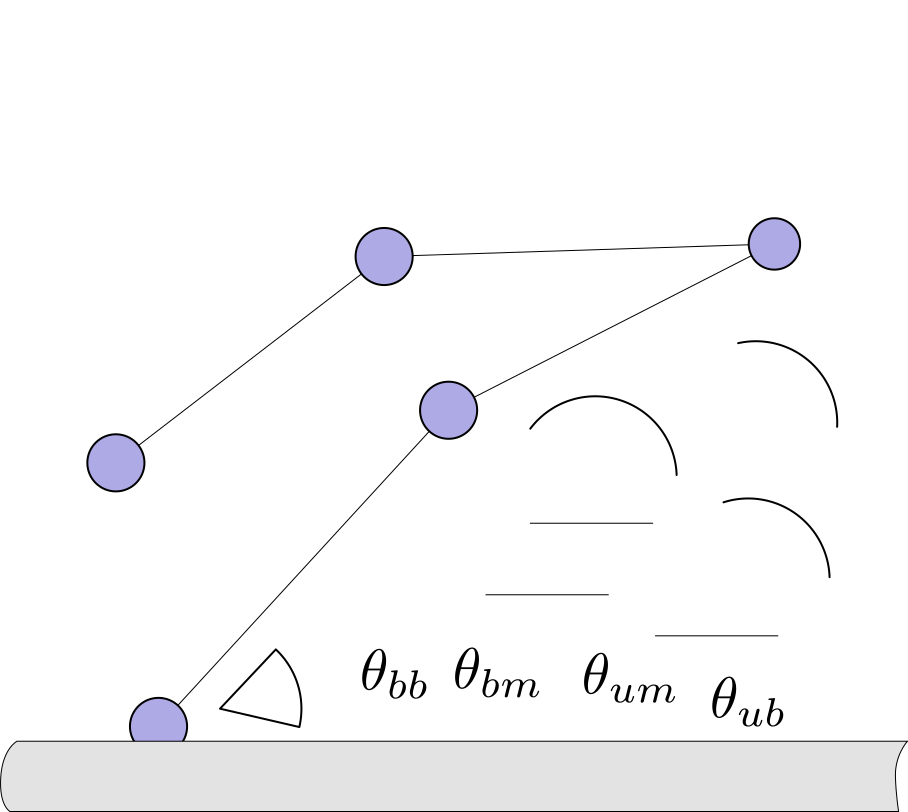
\includegraphics[width=.65\textwidth,keepaspectratio]{../../figures/ob_fig}
%%   \caption{Onebound dynein model.}{}
%%   \label{fig:model-intro}
%% \end{figure}

\subsubsection{Spherical domains connected by massless rods}
A key feature of the model is that each domain of the protein (two feet, twp motors and a tail) is treated as a sphere. Each sphere is connected to one or two other spheres, as shown in Figure (\ref{fig:model-intro}). This simplification is made to make the math easier and allow a simple definition of dynein's conformation.\\

One quickly notices by glancing at Figure (\ref{fig:crystal-structure-model-imposed}), a visualization of actual dynein, that modelling the tail and feet domains as spheres is a stretch. The main point of the simplification is not to capture the shape of dynein, but the conformation. It is undefined to discuss the distance between the two motor domains in real dynein, because the motors are made up of hundreds of amino acids, and the average inter-domain distance between amino acids is comparable to the intra-domain distance. However it is very easy to describe the difference between two spheres.\\

Each sphere has an associated drag factor $\gamma$, which describes the resistance it feels to motion. This drag factor is calculated based on the radius $R$ of the spheres, and is given by Stoke's Law:
%
\begin{equation}
  \gamma = 6\pi\nu R
\end{equation}
%
Thus R becomes a parameter input to the model.\\

\subsubsection{Rigid rods}
The model assumes connected domains are rigidly attached to one another by rods. This assumption makes the math easier, and is not necessarily based on biology. One study found that the standard deviation of stalk and stem lengths in \textit{in vitro} dynein was roughly $1nm$ \ref{burgess-paper}. However a contrasting piece of evidence showed the coiled coil, a common protein structure which links the MTBD and motor domains in dynein, can stretch in myosin, another motor protein, by 2.5x \ref{myosin-cc-elasticity}.

\subsubsection{Angular springs}
Each domain has a spring constant, $c_b, c_m$ or $c_t$ for binding, motor or tail, which decides the energy associated with that domain angle. For example, the tail domain energy is given by
%
\begin{equation}
  \Delta G_t = \frac12c_t\left(\theta_t - \theta_t^{eq}\right)^2
\end{equation}

\subsubsection{Two-state model}
The model assumes MT-bound dynein can assume one of two states: one where both MTBDs are bound, and one where only one MTBD is bound to the MT. These states are also differentiated by different motor equilibrium angles, $\Theta_{m}^{bb}$ and $\Theta_{m}^{ob}$, and different transition rates. Biological dynein likely passes through a series of permutations of nucleotide, MT affinity and conformational states as it travels through its mechanochemical cycle. This model makes the assumption that the mechanochemical cycle can be broken down into a cycle of prestroking to move the unbound foot forward, brownian walking to place the foot on the microtubule, then powerstroking to move the other domains forward.\\

\begin{figure}[h]
  \centering
  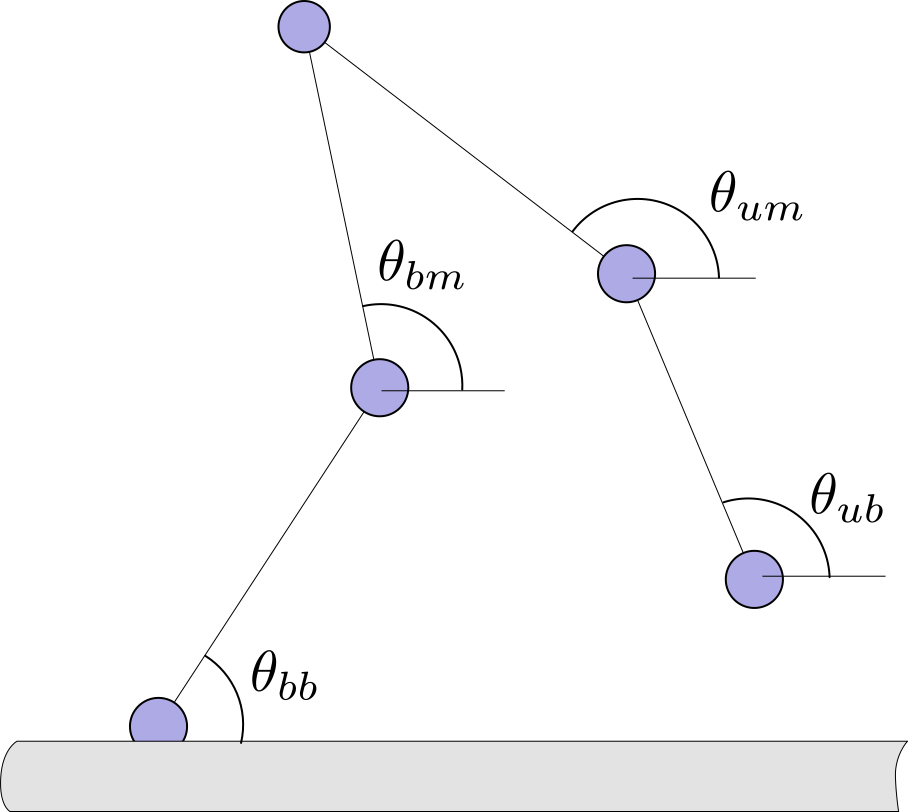
\includegraphics[width=.45\textwidth]{../../figures/code-onebound}
  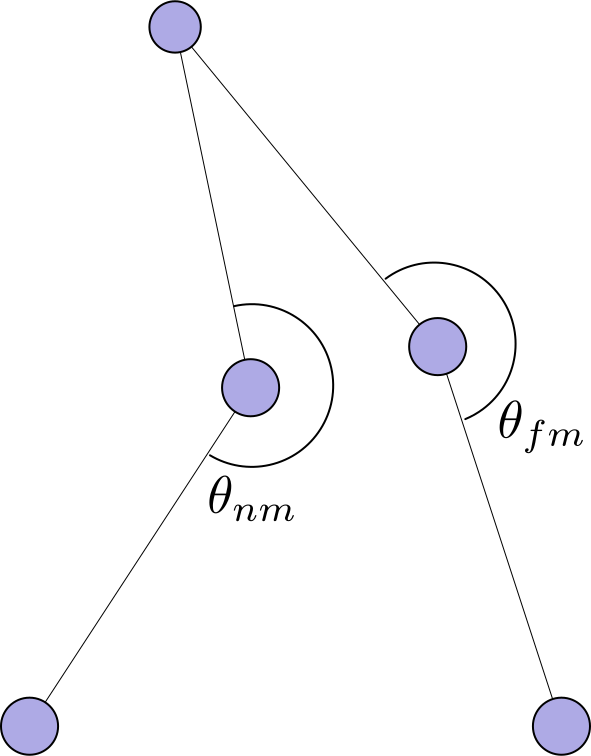
\includegraphics[width=.45\textwidth]{../../figures/code-bothbound}
  \caption{Dynein model schematics.}{Representations of onebound (left) and bothbound (right) dynein models.}
  \label{ob_fig}
\end{figure}

\textbf{todo: Add springs to joints!}

\subsubsection{Transitioning between states}
The model transitions between states with a probability dependent on both the energy difference between the two states and the physical separation between the MT and binding MTBD. The energy difference between states A and B is given by:
%
\begin{equation}
  \Delta G_{A\rightarrow B} = \sum_{i=0...N_B}^{B} \frac{1}{2}c_i\left(\theta_i-\Theta_i^B\right)^2 - \sum_{j=0...N_A}^{A} \frac{1}{2}c_j\left(\theta_j-\Theta_j^A\right)^2
\end{equation}
%
Transition energies are used to calculate transition rates, as given by the Arhennius equation $k=Ae^{-\beta\Delta G}$, where $\beta = (k_BT)^{-1}$. In this equation $\Delta G$ is the total energy of transition between states and A is a constant known as the preexponential factor with units of $s^{-1}$.\\
%
\begin{equation}
  k_b = Ae^{\frac{-\Delta G}{k_BT}} = Ae^{\frac{-\Delta G_{conf}}{k_BT}}e^{\frac{-\Delta G_{bind}}{k_BT}}
\end{equation}
%
where $\Delta G_{conf}$ is the change in spring energy in going from bothbound to onebound and $\Delta G_{bind}$ is the energy gained from binding to the microtubule. Because binding energy for the MT-MTBD complex is hard to find, the following substitution is made:
%
\begin{equation}
  k_b = Ae^{\frac{-\Delta G}{k_BT}} = Be^{\frac{-\Delta G_{conf}}{k_BT}}
\end{equation}
%
Thus $B$ becomes a parameter of the model.\\

\subsubsection{Brownian dynamics}
The Brownian dynamics equation describes the motion of high-drag objects which spend most of their time at terminal velocity, and is given by:
%
\begin{equation}
  \dot{x} = \frac{1}{\gamma}\left(F_{net} + R\right)
\end{equation}
%
where $\gamma$ is the drag constant of the object and $R$ is a random Brownian force which describes the effects of water particle collision. $R$ is a Gaussian-sampled zero-centered force with variance given by:
%
\begin{equation}
  R_{\sigma^2} = \sqrt{\frac{2*kb*T*\gamma}{dt}}
\end{equation}
%
Dynein is in the range of objects which BD describes well. (citation needed)

\subsubsection{Binding to microtubule}
The model ``steps'' whenever an MTBD diffuses near the microtubule. \textit{In vivo}, dynein binds to a site on the $\alpha-\beta$ tubulin polymer microtubule which repeats roughly every 8nm. Thus, all dynein steps should be multiples of $8$nm. This model ignores this requirement and allows stepping to occur at any length. The assumption is that \textit{in vivo} dynein takes 8nm steps because of its size and stepping angle. Thus the 8nm step length should be reproduced by the model without explicit coding.\\

\subsubsection{2D model}
The coordinate system for this model is two-dimensional. Thus interactions between the two motors and MTBDs are ignored. This assumption is made to simplify the model. Other dynein models, like the winch model \ref{sarlahmodel}, add in attractive and repulsive forces between the two motors which act in three dimensions. It is not clear why such forces are necessary for dynein motion, and so they are omitted.\\

Side stepping of dynein is ignored in this model. Stepping perpendicular to the MT occurs in dynein \cite{weihongppaer}, as shown in Figure \ref{fig:weihong-side-stepping}. This model assumes it is a symptom, and not an influencer of, of dynein's forward-backward stepping mechanism.

\begin{figure}[h]
  \centering
  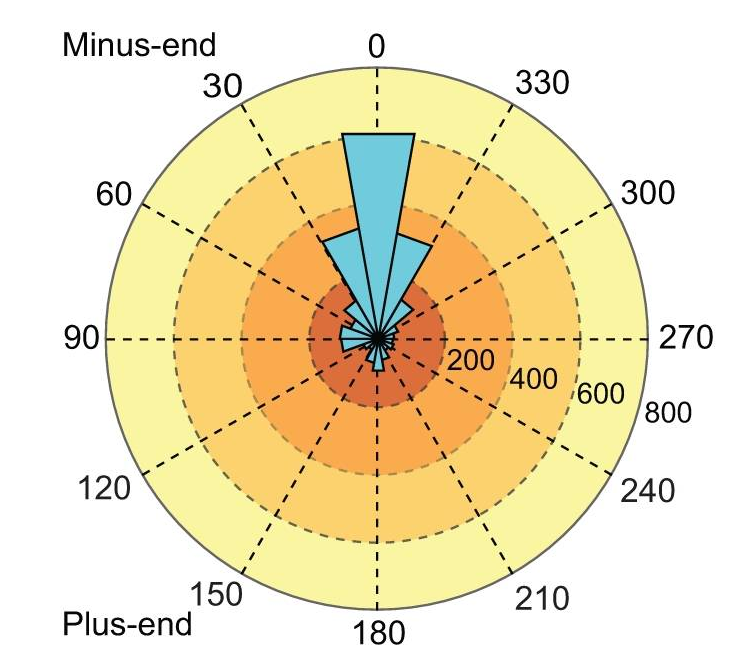
\includegraphics[width=.45\textwidth]{../../figures/weihong-side-stepping}
  \caption{Dynein experimental off-axis stepping histogram.}{Angular histogram of off-axis stepping of dynein, as found by \cite{weihongpaper}. 0 degrees corresponds to a step parallel to the MT, and 270 degrees a step purely to the right. Modified.}
  \label{fig:weihong-side-stepping}
\end{figure}

\subsection{Mathematical models}
To simulate a protein's passage through the above mechanochemical cycle, two mathematical models are needed: one for the prestroke, MTBD-detached state, and one for the poststroke, MTBD-bound state. The purpose of each model is to calculate the position and velocity of each domain at an arbitrary time.\\

\subsubsection{Prestroke onebound model}
Prestroke dynein is referred to as onebound, since one motor domain is bound to the MT in this state, and the other unbound. A spatial representation of onebound dynein is shown in Figure \ref{ob_fig}. 

%% \begin{figure}[h]
%%   \centering
%%   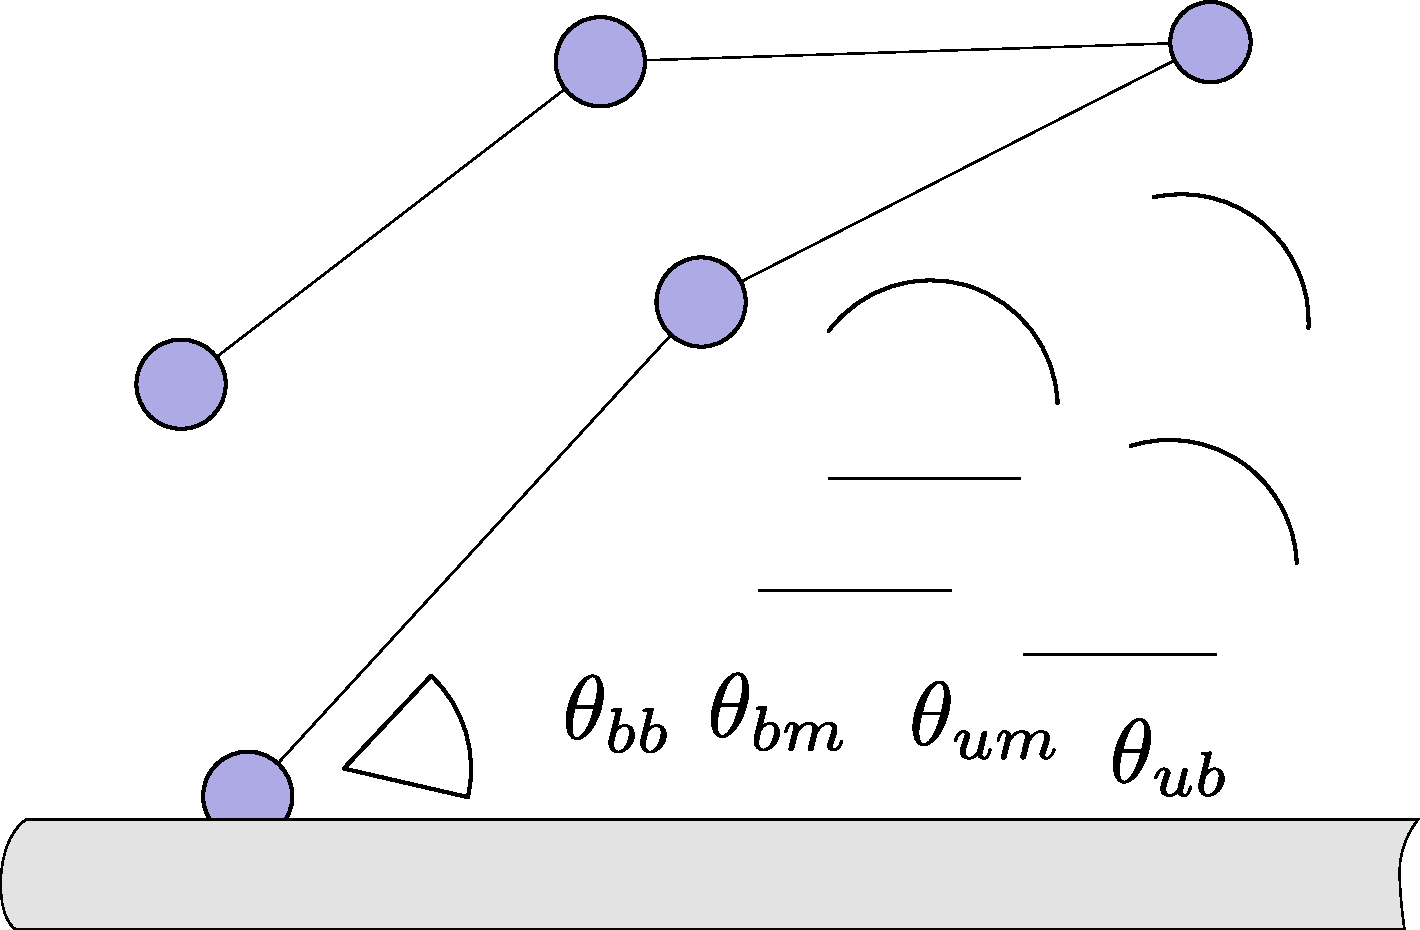
\includegraphics[width=.45\textwidth]{../../figures/ob_fig.pdf}
%%   \caption{Spatial representation of onebound model.}
%%   \label{ob_fig}
%% \end{figure}

TODO: make onebound model figure, label domain names (MTBD motor tail), Ls, Lt, microtubule\\

Each domain is represented by a point, and is connected to other domains via fixed-length rods. Angles represent the degrees of freedom of the model. Since the protein is a dimer, there are two copies of the MTB, motor and tail domains. The tails are fused together and so represented as a single point. The motor and MTB domains are given a ``bound'' and ``unbound'' designation to differentiate them. The ``bound'' domains are the MTBD attached to the MT and its corresponding motor domain. The unbound domains are the unbound MTBD and its corresponding motor domain.\\

\paragraph{Angular and Cartesian coordinates}

The four angles $\Theta_{bb}, \Theta_{bm}, \Theta_{um}$ and $\Theta_{ub}$, corresponding to bound binding, bound motor, unbound motor and unbound binding angle, together describe any possible conformation the system can take on. The domain of $\Theta_{bb}$ has a restricted domain of $[0,\pi]$ to prevent below-MT conformations, but the other angles have domains of $[0,2\pi]$. Each angle is defined relative to the horizontal axis. The position of the bound binding domain $X_{bb}$ and the four domain angles are all that is needed to determine the position of the protein at any time.\\

%% \begin{figure}[h]
%%   \centering
%%   \begin{tabular}{c}
%%     \begin{lstlisting}[language=C++]
%%       class Dynein_onebound{
%%         double &$\Theta_{bb}, \Theta_{bb}, \Theta_{bb}, \Theta_{bb}$&
%%         double &$\dot{\Theta}_{bb}, \dot{\Theta}_{bb}, \dot{\Theta}_{bb}, \dot{\Theta}_{bb}$&
%%         double &$X_{bb}$&
%%       }
%%     \end{lstlisting}
%%   \end{tabular}
%%   \caption{Pseudocode of the onebound Dynein model.}
%%   \label{ob_struct}
%% \end{figure}

\paragraph{$\dot{\Theta}_{ub}, \dot{\Theta}_{um}, \dot{\Theta}_{bm}, \dot{\Theta}_{bb}$ calculation}

The following equations allow recursive calculation of the positions of each domain in cartesian coordinates:

\noindent\begin{minipage}{0.49\linewidth}
\begin{align}
  X_{bm} &= X_{bb}+L_{s}\cos(\Theta_{bb}) \\
  X_{t}  &= X_{bm}+L_{t}\cos(\Theta_{bm}) \\
  X_{fm} &= X_{t} - L_{t}\cos(\Theta_{fm}) \\
  X_{fb} &= X_{fm} - L_{s}\cos(\Theta_{fb})
\end{align}
\end{minipage}
\begin{minipage}{0.49\linewidth}
\begin{align}
  Y_{bb} &= 0 \\
  Y_{bm} &= Y_{bb}+L_{s}\sin(\Theta_{bb}) \\
  Y_{t}  &= Y_{bm}+L_{t}\sin(\Theta_{bm}) \\
  Y_{fm} &= Y_{t} - L_{t}\sin(\Theta_{fm}) \\
  Y_{fb} &= Y_{fm} - L_{s}\sin(\Theta_{fb})
\end{align}
\end{minipage}
\vspace{.5cm}

$L_s$ and $L_t$ correspond to lengths of each interdomain rod, and the $t$ subscripts refer to tail domain coordinates.\\

\paragraph{Angular and Cartesian velocities}
The goal is to express angular velocities $\dot{\Theta}_{bb}, \dot{\Theta}_{bb}, \dot{\Theta}_{bb}$ and $\dot{\Theta}_{bb}$ in terms of known quantities. To begin, the cartesian velocities of each domain can be calculated from the above position equations in a similar recursive manner. A subset of the equations are shown here:

\noindent\begin{minipage}{0.49\linewidth}
\begin{align}
  \dot{X}_{bb} &= 0 \\
  \dot{X}_{bm} &= \dot{X}_{bb} - L_{s}\sin(\Theta_{bb})\dot{\Theta}_{bb} \label{cartesian-bmx}\\
  \dot{X}_{t } &= \dot{X}_{bm} - L_{t}\sin(\Theta_{bm})\dot{\Theta}_{bm}
  %% \dot{X}_{fm} &= \dot{X}_{t } + L_{t}\sin(\Theta_{fm})\dot{\Theta}_{fm} \\
  %% \dot{X}_{fb} &= \dot{X}_{fm} + L_{s}\sin(\Theta_{fb})\dot{\Theta}_{fb}
\end{align}
\end{minipage}
\begin{minipage}{0.49\linewidth}
\begin{align}                                                                          
  \dot{Y}_{bb} &= 0 \\                                                        
  \dot{Y}_{bm} &= \dot{Y}_{bb} + L_{s}\cos(\Theta_{bb})\dot{\Theta}_{bb} \\
  \dot{Y}_{t}  &= \dot{Y}_{bm} + L_{t}\cos(\Theta_{bm})\dot{\Theta}_{bm}
  %% \dot{Y}_{fm} &= \dot{Y}_{t } - L_{t}\cos(\Theta_{fm})\dot{\Theta}_{fm} \\
  %% \dot{Y}_{fb} &= \dot{Y}_{fm} - L_{s}\cos(\Theta_{fb})\dot{\Theta}_{fb}
\end{align}
\end{minipage}
\vspace{.5cm}

Another way to express these cartesian velocities is using the Brownian dynamics equation $\dot{X} = \frac1\gamma F_{net} + R$:

\begin{align}  
  \dot{X}_{bm} &= \frac{1}{\gamma_m} \Big(F_{xml} + - \lambda_{bs}(X_{bm} - X_{bb}) + \lambda_{bt}(X_{t } - X_{bm}) \Big) + R_{xml} \label{brownian-bmx}\\
  \dot{X}_{t } &= \frac{1}{\gamma_t} \Big(F_{xt } + - \lambda_{bt}(X_{t } - X_{bm}) + \lambda_{ft}(X_{fm} - X_{t }) \Big) + R_{xt }
  %% \dot{X}_{fm} &= \frac{1}{\gamma_m} \Big(F_{xmr} + - \lambda_{ft}(X_{fm} - X_{t }) + \lambda_{fs}(X_{fb} - X_{fm}) \Big) + R_{xmr} \\
  %% \dot{X}_{fb} &= \frac{1}{\gamma_b} \Big(F_{xbr} + - \lambda_{fs}(X_{fb} - X_{fm}) \Big) + R_{xbr}
\end{align}

%% \begin{align}  
%%   \dot{Y}_{bm} &= \frac{1}{\gamma_m} \Big(F_{yml} + - \lambda_{bs}(Y_{bm} - Y_{bb}) + \lambda_{bt}(Y_{t } - Y_{bm}) \Big) + R_{yml} \\
%%   \dot{Y}_{t}  &= \frac{1}{\gamma_t} \Big(F_{yt } + - \lambda_{bt}(Y_{t } - Y_{bm}) + \lambda_{ft}(Y_{fm} - Y_{t }) \Big) + R_{yt } \\
%%   \dot{Y}_{fm} &= \frac{1}{\gamma_m} \Big(F_{ymr} + - \lambda_{ft}(Y_{fm} - Y_{t }) + \lambda_{fs}(Y_{fb} - Y_{fm}) \Big) + R_{ymr} \\
%%   \dot{Y}_{fb} &= \frac{1}{\gamma_b} \Big(F_{ybr} + - \lambda_{fs}(Y_{fb} - Y_{fm}) \Big) + R_{ybr}
%% \end{align}

where $\gamma_n$ is a drag coefficient for the binding, motor or tail domain with units of mass per second. $F_{xn}$ is the x component of external force on each domain $n$ due to various factors. $\lambda_{12}\left(X_1 - X_2\right)$ is the x component of internal force on domain $2$ due to domain $1$, where $\lambda$ is a tension coefficient with units of mass per second per second. $R_{xn}$ is the Brownian coefficient representing motion due to solvent collision, with units of velocity.\\

These two sets of equations, cartesian and Brownian, can be equated to get more interesting equations. For example, Eq (\ref{cartesian-bmx}) and Eq (\ref{brownian-bmx}) can be equated. This equating, combined with expanding the recursive velocity definitions leads to new equations, some of which are shown here:

\begin{align}
  &-L_s\sin(\theta_{bb})\dot{\theta}_{bb} = \frac{1}{\gamma_m}F_{xml} + -\frac{1}{\gamma_m}\lambda_{bs}(X_{bm} - X_{bb}) + \frac{1}{\gamma_m}\lambda_{bt}(X_{t } - X_{bm}) + R_{bmx} \label{ob_system_first}\\
  &-L_s\sin(\theta_{bb})\dot{\theta}_{bb} - L_t\sin(\theta_{bm})\dot{\theta}_{bm} = \frac{1}{\gamma_t}F_{xt } + -\frac{1}{\gamma_t}\lambda_{bt}(X_{t } - X_{bm}) + \frac{1}{\gamma_t}\lambda_{ft}(X_{um} - X_{t }) + R_{tx}
  %% &-L_s\sin(\theta_{bb})\dot{\theta}_{bb} - L_t\sin(\theta_{bm})\dot{\theta}_{bm} + L_t\sin(\theta_{um})\dot{\theta}_{um} = \frac{1}{\gamma_m}F_{xmr} + -\frac{1}{\gamma_m}\lambda_{ft}(X_{um} - X_{t }) + \frac{1}{\gamma_m}\lambda_{fs}(X_{ub} - X_{um}) + R_{bmx} \\
  %% &-L_s\sin(\theta_{bb})\dot{\theta}_{bb} - L_t\sin(\theta_{bm})\dot{\theta}_{bm} + L_t\sin(\theta_{um})\dot{\theta}_{um} + L_s\sin(\theta_{ub})\dot{\theta}_{ub} = \frac{1}{\gamma_b}F_{xbr} + -\frac{1}{\gamma_b}\lambda_{fs}(X_{ub} - X_{um}) + R_{bbx}
\end{align}

%% \begin{align}
%%   &L_s\cos(\theta_{bb})\dot{\theta}_{bm} = \frac{1}{\gamma_m}F_{yml} + -\frac{1}{\gamma_m}\lambda_{bs}(Y_{bm} - Y_{bb}) + \frac{1}{\gamma_m}\lambda_{bt}(Y_{t } - Y_{bm}) + R_{umy} \\
%%   &L_s\cos(\theta_{bb})\dot{\theta}_{bb} + L_t\cos(\theta_{bm})\dot{\theta}_{bm} = \frac{1}{\gamma_t}F_{yt } + -\frac{1}{\gamma_t}\lambda_{bt}(Y_{t } - Y_{bm}) + \frac{1}{\gamma_t}\lambda_{ft}(Y_{um} - Y_{t }) + R_{ty} \\
%%   &L_s\cos(\theta_{bb})\dot{\theta}_{bb} + L_t\cos(\theta_{bm})\dot{\theta}_{bm} - L_t\cos(\theta_{um})\dot{\theta}_{um} = \frac{1}{\gamma_m}F_{ymr} + -\frac{1}{\gamma_m}\lambda_{ft}(Y_{um} - Y_{t }) + \frac{1}{\gamma_m}\lambda_{fs}(Y_{ub} - Y_{um}) + R_{bmy} \\
%%   &L_s\cos(\theta_{bb})\dot{\theta}_{bb} + L_t\cos(\theta_{bm})\dot{\theta}_{bm} - L_t\cos(\theta_{um})\dot{\theta}_{um} - L_s\cos(\theta_{ub})\dot{\theta}_{ub} = \frac{1}{\gamma_b}F_{ybr} + -\frac{1}{\gamma_b}\lambda_{fs}(Y_{ub} - Y_{um}) + R_{bby} \label{ob_system_last}
%% \end{align}

A total of eight coupled differential equations are formed from this procedure. These eight equations form a system of equations with eight unknowns: $\dot{\Theta}_{bb}, \dot{\Theta}_{bb}, \dot{\Theta}_{bb}$ and $\dot{\Theta}_{bb}$, and the four tension coefficients $\lambda_{bs}, \lambda_{bt}, \lambda_{um}$ and $\lambda_{ub}$. This system is more compactly represented as:
{\small
  \[
  \hspace{-1.0cm}
  \resizebox{0.85\linewidth}{!}{%
  $\begin{pmatrix}
    L_s\sin\theta_{bb} & 0 & 0 & 0 & -\gamma_m (X_{bm} - X_{bb}) & \gamma_m (X_{t } - X_{bm}) & 0 & 0\\
    L_s\sin(\theta_{bb}) & L_t\sin(\theta_{bm}) & 0 & 0 & 0 & -\gamma_t (X_{t } - X_{bm}) & \gamma_t (X_{um} - X_{t }) & 0\\
    L_s\sin(\theta_{bb}) & L_t\sin(\theta_{bm}) & -L_t\sin(\theta_{um}) & 0 & 0 & 0 & -\gamma_m (X_{um} - X_{t }) & \gamma_m (X_{ub} - X_{um})\\
    L_s\sin(\theta_{bb}) & L_t\sin(\theta_{bm}) & -L_t\sin(\theta_{um}) & -L_s\sin(\theta_{ub}) & 0 & 0 & 0 & -\gamma_b (X_{ub} - X_{um})\\
    -L_s\cos(\theta_{bb}) & 0 & 0 & 0 & -\gamma_m (Y_{bm} - Y_{bb}) & \gamma_m (Y_{t } - Y_{bm}) & 0 & 0\\
    -L_s\cos(\theta_{bb}) & -L_t\cos(\theta_{bm}) & 0 & 0 & 0 & -\gamma_t (Y_{t } - Y_{bm}) & \gamma_t (Y_{um} - Y_{t }) & 0\\
    -L_s\cos(\theta_{bb}) & -L_t\cos(\theta_{bm}) & L_t\cos(\theta_{um}) & 0 & 0 & 0 & -\gamma_m (Y_{um} - Y_{t }) & \gamma_m (Y_{ub} - Y_{um})\\
    -L_s\cos(\theta_{bb}) & -L_t\cos(\theta_{bm}) & L_t\cos(\theta_{um}) & L_s\cos(\theta_{ub}) & 0 & 0 & 0 & -\gamma_b (Y_{ub} - Y_{um})\\
  \end{pmatrix}$%
  }
  \begin{pmatrix}
    \dot{\theta}_{bb}\\
    \dot{\theta}_{bm}\\
    \dot{\theta}_{um}\\
    \dot{\theta}_{ub}\\
    \lambda_{bs}\\
    \lambda_{bt}\\
    \lambda_{ut}\\
    \lambda_{us}\\
  \end{pmatrix}
  =
  \begin{pmatrix}
    -F_{bmx} + \gamma_m R_{bmx}\\
    -F_{tx} + \gamma_t R_{tx}\\
    -F_{umx} + \gamma_m R_{umx}\\
    -F_{ubx} + \gamma_b R_{ubx}\\
    -F_{bmy} + \gamma_m R_{bmy}\\
    -F_{ty} + \gamma_t R_{ty}\\
    -F_{umy} + \gamma_m R_{umy}\\
    -F_{uby} + \gamma_b R_{uby}\\
  \end{pmatrix}
  \]
}

This matrix is then solved using the Mathematica computer algebra system, resulting in a set of motion equations which describe the model's trajectory over time, eg $\dot{\Theta_{bm}}(\Theta_{bb}, \Theta_{bm}, \Theta_{um}, \Theta_{ub})$. These motion equations are further described in (\ref{sec:ob-motion-equations}).\\

\subsubsection{Poststroke bothbound model}
The main difference between the prestroke and poststroke mathematical models is that the latter has a further constraint: both its MTB domains are attached to the MT. This has the effect of diminishing the degrees of freedom of the system from four to two, assuming the motor remains above the MT. A spatial representation of the bothbound model is shown in Figure (\ref{bb_fig}).\\

\begin{figure}[h]
  \centering
  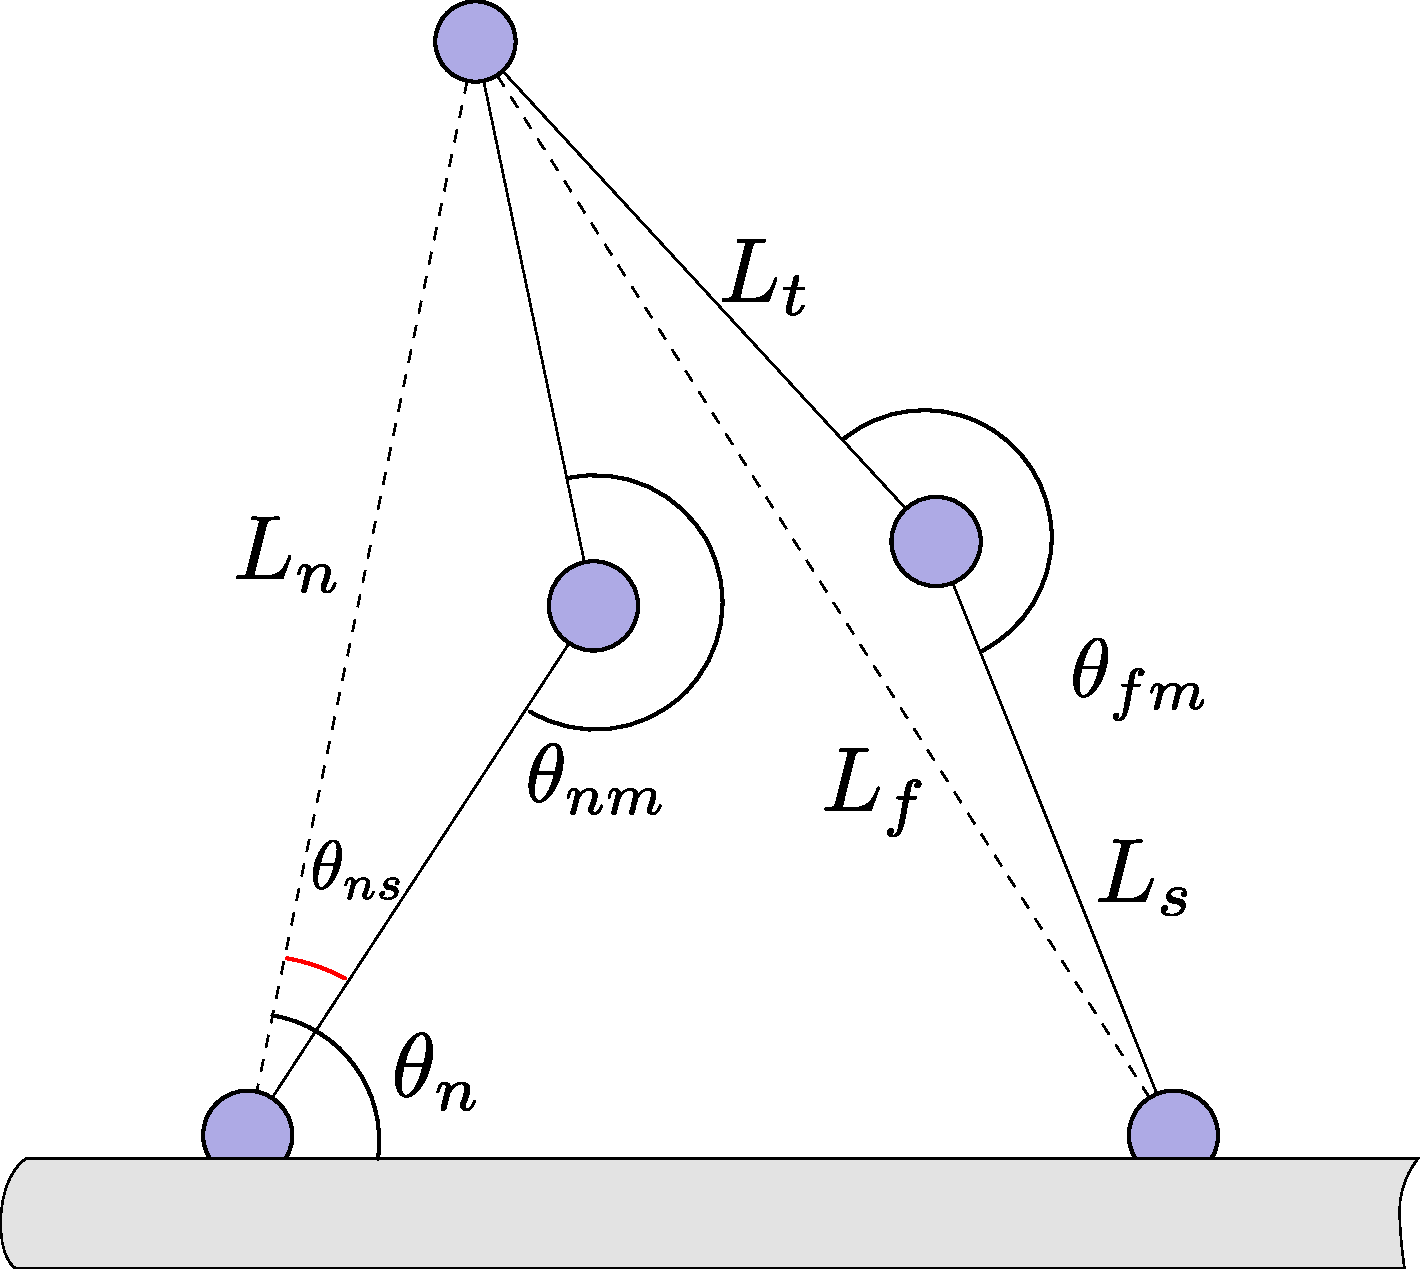
\includegraphics[width=.45\textwidth]{../../figures/code-bothbound.pdf}
  \caption{Model bothbound equilibrium angle defintion.}{}
  \label{bb_fig}
\end{figure}

The bothbound model is very similar in assumptions to the onebound: domains are represented as points connected by rigid rods, and the tails are still fused into a single point. The main differences are the naming scheme and spatial constraints. Dimers can no longer be differentiated by being un/bound, so are now differentiated by their z-position: being near or far from the ``camera.'' This is similar to labeling them as the right or left dimer. Thus there are the near binding (nb), near motor (nm), tail (t), far motor (fm) and far binding (fb) domains. Both the near and far binding domains have their x-coordinate fixed at zero. The system is described completely by two angles: $\Theta_{nm}$ and $\Theta_{fm}$. Angles $\Theta_t, \Theta_{nb}$ and $\Theta_{fb}$ are dependent on these two motor angles.\\

The second MTBD constraint adds another required piece of information the model must track: the x position of the second MTBD. This position is described by $L$, the distance between the near and far binding domains. The pseudocode used to describe the bothbound model are shown in Figure (\ref{bb_struct}).\\

\begin{figure}[h]
  \centering
  \begin{tabular}{c}
    \begin{lstlisting}[language=C++]
      class Dynein_bothbound{
        double &$\Theta_{nm}, \Theta_{fm}$&
        double &$\dot{\Theta}_{nm}, \dot{\Theta}_{fm}$&
        double &$X_{nb, L}$&
      }
    \end{lstlisting}
  \end{tabular}
  \caption{Pseudocode of the bothbound Dynein model.}
  \label{ob_struct}
\end{figure}

\paragraph{$\dot{\Theta}_{nm}, \dot{\Theta}_{fm}$ calculation}

The first step in calculating angular velocities is to define new variables $L_n$ and $L_f$ using the Law of Cosines:

\begin{align}
  L_n &= \sqrt{L_s^2 + L_t^2 - 2L_sL_t\cos{\theta_{nm}}} \\
  L_f &= \sqrt{L_s^2 + L_t^2 - 2L_sL_t\cos{\theta_{fm}}}
\end{align}

These new artificial stalks are not physically relevant, but allow the definition of new angles $\Theta_n, \Theta_{ns}, \Theta_{f}$ and $\Theta_{fs}$, which are useful for calculating the position of the motor domain. The treatment of the near and far versions of these angles is very similar, so only the near angles will be dealt with here. The angles themselves are never dealt with, only their $\sin$s and $\cos$s:

\begin{align}
  \cos\theta_n &= \frac{L^2 + L_n^2 - L_f^2}{2L L_n} \\
  \sin\theta_{n} &= \sqrt{1 - \cos^2\theta_{n}} \\
  \cos\theta_{ns} &= \frac{L_s^2 + L_n^2 - L_t^2}{2L_s L_n} \\
  \sin\theta_{ns} &=
  \begin{cases}
    +\sqrt{1 - \cos^2\theta_{ns}} & \theta_{nm} < \pi \\
    -\sqrt{1 - \cos^2\theta_{ns}} & \theta_{nm} > \pi
  \end{cases}
\end{align}

These values are arrived at through the Law of Cosines and a trigonometric identity. The sign of $\sin\left(\Theta_n\right)$ is restricted to positive values due to the angle's $[0,\pi]$ domain. $\Theta_{ns}$'s domain is $[-\pi,\pi]$, meaning its sign is not restricted. The partial derivatives of these values are used in future calculations, and some are shown here:

\begin{align}
  \frac{\partial \cos\theta_n}{\partial L_n} &= \frac{1}{L} - \frac{L^2 + L_n^2 - L_f^2}{2L L_n^2}\\
  \frac{\partial \cos\theta_n}{\partial L_f} &= -\frac{L_f}{LL_n}\\
  \frac{\partial \sin\theta_n}{\partial L_n} &= \frac{-\cos\theta_n}{\sqrt{1-\cos^2\theta_n}}
  \left(\frac{1}{L} - \frac{L^2 + L_n^2 - L_f^2}{2L L_n^2}\right)
  %% \frac{\partial \sin\theta_n}{\partial L_f} &= \frac{-\cos\theta_n}{\sqrt{1-\cos^2\theta_n}}
  %% \left(\frac{-L_f}{LLn}\right)\\
  %% \frac{\partial \cos\theta_{ns}}{\partial L_n} &= \frac{1}{L_s}
  %% - \frac{L_s^2 + L_n^2 - L_t^2}{2L_sL_n^2}\\
  %% \frac{\partial \cos\theta_{ns}}{\partial L_f} &= 0\\
  %% \frac{\partial \sin\theta_{ns}}{\partial L_n} &=
  %% \begin{cases}
  %%   \frac{-\cos\theta_{ns}}{\sqrt{1-\cos^2\theta_{ns}}}
  %%   \left(\frac{1}{L_s} - \frac{L_s^2+L_n^2-L_t^2}{2LL_n^2}\right) & \theta_{nm} < \pi \\
  %%   \frac{\cos\theta_{ns}}{\sqrt{1-\cos^2\theta_{ns}}}
  %%   \left(\frac{1}{L_s} - \frac{L_s^2+L_n^2-L_t^2}{2LL_n^2}\right) & \theta_{nm} > \pi
  %% \end{cases}\\
  %% \frac{\partial \sin\theta_{ns}}{\partial L_f} &= 0
\end{align}

The position of the motor and tail domains is calculated as follws, using the angle addition trigonometric identity:

\begin{align}
  X_{nm} &= L_s\left(
  \cos\theta_n\cos\theta_{ns} - \sin\theta_n\sin\theta_{ns}
  \right)
  \\
  Y_{nm} &= L_s\left(
  \cos\theta_n\sin\theta_{ns} + \sin\theta_n\cos\theta_{ns}
  \right)
  \\
  X_{t} &= L_n\cos\theta_n\\
  Y_{t} &= L_n\sin\theta_n
\end{align}

The partial derivatives of these values are used later. A selection are shown here:

\begin{align}
  \frac{dX_{nm}}{dL_n} &= L_s\Big(\cos\theta_n\frac{d\cos\theta_{ns}}{dL_n} + \cos\theta_{ns}\frac{d\cos\theta_{n}}{dL_n} - \sin\theta_n\frac{d\sin\theta_{ns}}{dL_n} - \sin\theta_{ns}\frac{d\sin\theta_{n}}{dL_n}\Big)\\
  \frac{dY_{nm}}{dL_n} &= L_s\Big(\cos\theta_n\frac{d\sin\theta_{ns}}{dL_n} + \sin\theta_{ns}\frac{d\cos\theta_{n}}{dL_n} + \sin\theta_n\frac{d\cos\theta_{ns}}{dL_n} + \cos\theta_{ns}\frac{d\sin\theta_{n}}{dL_n} \Big)\\
  \frac{dX_{nm}}{dL_f} &= L_s\Big(\cos\theta_n\frac{d\cos\theta_{ns}}{dL_f} + \cos\theta_{ns}\frac{d\cos\theta_{n}}{dL_f} - \sin\theta_n\frac{d\sin\theta_{ns}}{dL_f} - \sin\theta_{ns}\frac{d\sin\theta_{n}}{dL_f} \Big)
  %% \frac{dY_{nm}}{dL_f} &= L_s\Big(\cos\theta_n\frac{d\sin\theta_{ns}}{dL_f} + \sin\theta_{ns}\frac{d\cos\theta_{n}}{dL_f} + \sin\theta_n\frac{d\cos\theta_{ns}}{dL_f} + \cos\theta_{ns}\frac{d\sin\theta_{n}}{dL_f}\Big)\\
  %% \frac{dX_{t}}{dL_n} &= \cos\theta_n + L_n\frac{\partial \cos\theta_n}{\partial L_n} = \frac{L_n}{L}\\
  %% \frac{dY_{t}}{dL_n} &= \sin\theta_n + L_n\frac{\partial \sin\theta_n}{\partial L_n}\\
  %% \frac{dX_{t}}{dL_f} &= L_n\frac{\partial \cos\theta_n}{\partial L_f} = -\frac{L_f}{L}\\
  %% \frac{dY_{t}}{dL_f} &= L_n\frac{\partial \sin\theta_n}{\partial L_f}\\
\end{align}

These partial derivatives are then used in a system of equations very similar to that in Equations (\ref{ob_system_first}-\ref{ob_system_last}), combining Brownian and coordinate system definitions of domain velocities:

\begin{align}
  \dot{X}_{nm} &= \frac{1}{\gamma} \Big(F_{xml} - \lambda_{ns}(X_{bm} - X_{bb})
  + \lambda_{nt}(X_{t } - X_{bm}) \Big) + R_{xml}
  &=& \frac{\partial X_{nm}}{\partial L_n}\dot{L}_n + \frac{\partial X_{nm}}{\partial L_f}\dot{L}_f\\
  \dot{X}_{t } &= \frac{1}{\gamma} \Big(F_{xt } - \lambda_{nt}(X_{t } - X_{bm})
  + \lambda_{ft}(X_{fm} - X_{t }) \Big) + R_{xt }
  &=& \frac{\partial X_{t}}{\partial L_n}\dot{L}_n + \frac{\partial X_{t}}{\partial L_f}\dot{L}_f\\
  \dot{X}_{fm} &= \frac{1}{\gamma} \Big(F_{xmr} - \lambda_{ft}(X_{fm} - X_{t })
  + \lambda_{fs}(X_{fb} - X_{fm}) \Big) + R_{xmr}
  &=& \frac{\partial X_{fm}}{\partial L_n}\dot{L}_n + \frac{\partial X_{fm}}{\partial L_f}\dot{L}_f
\end{align}

\begin{align}
  \dot{Y}_{nm} &= \hspace{1cm} \frac{1}{\gamma} \Big(F_{yml} - \lambda_{ns}(Y_{bm} - Y_{bb})
  + \lambda_{nt}(Y_{t } - Y_{bm}) \Big) + R_{yml}
  &= \frac{\partial Y_{nm}}{\partial L_n}\dot{L}_n + \frac{\partial Y_{nm}}{\partial L_f}\dot{L}_f\\
  \dot{Y}_{t}  &= \hspace{1cm} \frac{1}{\gamma} \Big(F_{yt } - \lambda_{nt}(Y_{t } - Y_{bm})
  + \lambda_{ft}(Y_{fm} - Y_{t }) \Big) + R_{yt }
  &= \frac{\partial Y_{t}}{\partial L_n}\dot{L}_n + \frac{\partial Y_{t}}{\partial L_f}\dot{L}_f\\
  \dot{Y}_{fm} &= \hspace{1cm} \frac{1}{\gamma} \Big(F_{ymr} - \lambda_{ft}(Y_{fm} - Y_{t })
  + \lambda_{fs}(Y_{fb} - Y_{fm}) \Big) + R_{ymr}
  &= \frac{\partial Y_{fm}}{\partial L_n}\dot{L}_n + \frac{\partial Y_{fm}}{\partial L_f}\dot{L}_f
\end{align}

The matrix version of this system looks like:

\[
\begin{pmatrix}
  -\frac{X_{nm}}{Ln} & -\frac{X_{nm}}{Lf}
  & -\frac{X_{nm}-X_{nb}}{\gamma} & \frac{X_{t}-X_{nm}}{\gamma} & 0 & 0\\
  -\frac{X_{t}}{Ln} & -\frac{X_{t}}{Lf}
  & 0 & -\frac{X_{t}-X_{nm}}{\gamma} & \frac{X_{fm}-X_{t}}{\gamma} & 0\\
  -\frac{X_{fm}}{Ln} & -\frac{X_{fm}}{Lf}
  & 0 & 0 & -\frac{X_{fm}-X_{t}}{\gamma} & \frac{X_{fb}-X_{fm}}{\gamma}\\
  -\frac{Y_{nm}}{Ln} & -\frac{Y_{nm}}{Lf}
  & -\frac{Y_{nm}-Y_{nb}}{\gamma} & \frac{Y_{t}-Y_{nm}}{\gamma} & 0 & 0\\
  -\frac{Y_{t}}{Ln} & -\frac{Y_{t}}{Lf}
  & 0 & -\frac{Y_{t}-Y_{nm}}{\gamma} & \frac{Y_{fm}-Y_{t}}{\gamma} & 0\\
  -\frac{Y_{fm}}{Ln} & -\frac{Y_{fm}}{Lf}
  & 0 & 0 & -\frac{Y_{fm}-Y_{t}}{\gamma} & \frac{Y_{fb}-Y_{fm}}{\gamma}\\
\end{pmatrix}
\begin{pmatrix}
  \dot{L}_n\\
  \dot{L}_f\\
  \lambda_{ns}\\
  \lambda_{nt}\\
  \lambda_{ft}\\
  \lambda_{fs}\\
\end{pmatrix}
=
\begin{pmatrix}
  -\frac{1}{\gamma}F_{nmx} - R_{nmx}\\
  -\frac{1}{\gamma}F_{tx}  - R_{tx}\\
  -\frac{1}{\gamma}F_{fmx} - R_{fmx}\\
  -\frac{1}{\gamma}F_{nmy} - R_{nmy}\\
  -\frac{1}{\gamma}F_{ty}  - R_{ty}\\
  -\frac{1}{\gamma}F_{fmy} - R_{fmy}\\
\end{pmatrix}
\]

This system of equations is then solved and used to calculate $\dot{L}_n$ and $\dot{L}_f$, as shown in Appendix (\ref{sec:bb-motion-equations}).

\subsection{Data interpretation}
Metrics for quality are required to assess how well the model fits reality. These metrics include time spent in one/bothbound states and average step size. These metrics are developed here.\\

\subsubsection{Converting experimental rates to preexponential factors $A_b$ and $A_{ub}$}
Rate constants $k_b$ and $k_{ub}$ govern the probability of transitioning from onebound to bothbound and vice-versa, respectively. One issue is that when these parameters are measured experimentally, the values represent the average rate for an ensemble of dynein in many different conformations. In contrast, the rates the model uses represent the probability of unbinding of a specific conformation. Thus, it is necessary to find a way to convert between experimental rates $k_b^{exp}$ and $k_{ub}^{exp}$ and conformation-specific rates $k_b$ and $k_{ub}$. As shown in Section \ref{sec:transitioning-states}, rates can be expressed using the Arrhenius equation:

\begin{align*}
  k_b &= A_b'e^{\frac{-\Delta G_{bind}}{k_BT}} = A_b'e^{\frac{-\Delta G_{conf}^{ob\rightarrow bb}}{k_BT}}e^{\frac{-\Delta G_{bind}}{k_BT}} = A_be^{\frac{-\Delta G_{conf}^{ob\rightarrow bb}}{k_BT}}\\
  k_{ub} &= A_{ub}'e^{\frac{-\Delta G_{unbind}}{k_BT}} = A_{ub}'e^{\frac{-\Delta G_{conf}^{bb\rightarrow ob}}{k_BT}}e^{\frac{\Delta G_{bind}}{k_BT}} = A_{ub}e^{\frac{-\Delta G_{conf}^{bb\rightarrow ob}}{k_BT}}
\end{align*}

where the constant Boltzmann factor for binding energy are hidden inside the unprimed preexponential factors. The experimental values are calculated the same way, with the free energy changes replaced with expectation values. Since by the equipartition theorem $\left<G_{conf}^{ob}\right> = 2k_BT$ and $\left<G_{conf}^{bb}\right> = k_BT$, the equations can be simplified:

\begin{align*}
  k_b^{exp} &= A_be^{\frac{-\left(2k_BT - k_BT\right)}{k_BT}} = \frac{A_b}{e}\\
  k_{ub}^{exp} &= A_{ub}e^{\frac{-\left(k_BT-2k_BT\right)}{k_BT}} = A_{ub}e
\end{align*}

Thus experimental rates can be converted easily into the model parameters $A_b$ and $A_{ub}$.

\subsubsection{Literature values for experimental binding rates}
Sarlah \textit{et. al.} \cite{sarlahmodel} perform a similar simulation of dynein and provide the reaction rates shown in Figure \ref{fig:sarlah-rate-table}.

\begin{figure}[h]
  \centering
  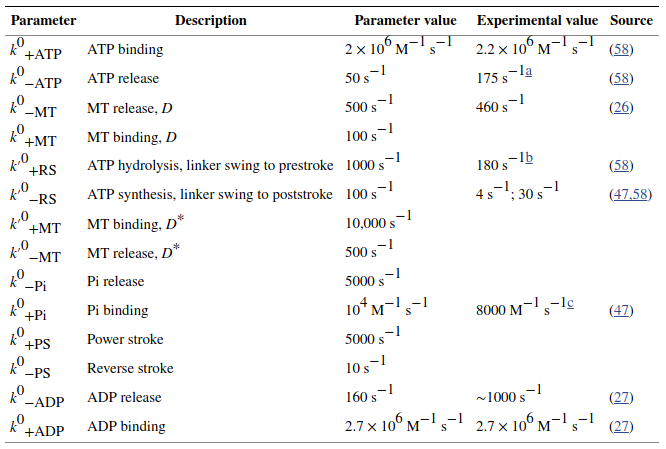
\includegraphics[width=.45\textwidth]{../../figures/SarlahParameterTable.png}
  \caption{Sarlah kinetic rates.}{Kinetic rates used in Sarlah \textit{et. al.}'s model \cite{sarlahmodel}.}
  \label{fig:sarlah-rate-table}
\end{figure}

The assumption of this project is that many of the states in this table can be combined into a single state without loss of predictive power of dynein behavior. Specifically, the assumption is that ejecting phosphate, conducting the powerstroke, releasing ADP, binding ATP and dissociating from the microtubule and all occur during the bothbound state, and hydrolyzing ATP, conducting the prestroke and rebinding the MT occur during onebound. These states are roughly grouped as MT-bound and MT-unbound states in the Cianfrocco mechanochemical cycle \cite{cianfroccoreview}.\\

The rate-limiting transitions in the Cianfrocco model are used as the guess $k_b$ and $k_{ub}$ values. That means that, since ATP hydrolysis has the slowest rate constant in onebound and MT release has the slowest rate in bothbound, $k_b^{exp} = 180 s^{-1}$ and $k_{ub} = 460 s^{-1}$ serve as good initial guesses.\\

\subsubsection{Calculating one/bothbound times of experimental dynein}
Rate constants can be fit to experimentally measurable values, such as velocity and the time dynein is bound to the microtubule (processivity time). We define the following values:

\newcommand\tbb{\left<t_{bb}\right>}
\newcommand\tob{\left<t_{ob}\right>}
\newcommand\tstep{\left<t_{step}\right>}
\newcommand\tproc{\left<t_{processivity}\right>}
\newcommand\kub{k_{ub}}
\newcommand\kb{k_{b}}
\newcommand\ko{k_{dis}}

\begin{itemize}
\item $\tbb$: Time in bothbound per step
\item $\tob$: Time in onebound per step
\item $\tstep$: Time of a single step. $\tstep=\tbb+\tob$.
\item $P_{bb}$: Probability of being bothbound per unit time. $P_{bb} = \frac{\tbb}{\tstep}$
\item $P_{ob}$: Probability of being onebound per unit time. $P_{ob} = \frac{\tob}{\tstep}$
\item $\kub$: Rate of unbinding per unit time while in bothbound. $\kub = \tbb^{-1}$
\item $\kb$: Rate of binding per unit time while in onebound. $\kb = \tob^{-1}$
\item $\ko$: Rate of unbinding per unit time while in onebound. $\ko = P_{ob}\kub$
\item $\tproc$: Time bound to microtubule before dissociation. step length / velocity $= \ko^{-1}$
\end{itemize}

$\tbb$ and $\tob$ can thus be defined in terms of observables $\tstep$ and $\tproc$:

\begin{align*}
  \ko &= P_{ob}\kub = \frac{\tob}{\tstep\tbb}\\
  &= \frac{\tstep-\tbb}{\tstep\tbb}\\
  &= \frac{\tstep-\tbb}{\tstep\tbb}\\
  \tproc &= \frac{\tstep\tbb}{\tstep-\tbb}\\
  \tbb &= \frac{\tproc\tstep}{\tproc+\tstep}\\
  \tob &= \tstep-\tbb\\
  &= \tstep - \frac{\tstep\tproc}{\tstep+\tproc}\\
  &= \frac{\tstep^2}{\tstep+\tproc}\\
\end{align*}

Thus, by the above equations and using data from \cite{weihongpaper}, values for $\tbb$ and $\tob$ can be found:

\begin{figure}[h]
  \centering
  \begin{tabular}{| c | c | c | c | c | c |}
    \hline
    Velocity & $\left<L_{step}\right>$ & $\tstep$ & $\tproc$ & $\tbb$ & $\tob$ \\ \hline
    134nm/s & 8nm & 0.06s & 7.9s & 0.0595s & 4.52e-4\\ \hline
  \end{tabular}
  \caption{Experimental values for fitting.}{Table calculating estimates for $\tbb$ and $\tob$.}
  \label{table:time-parameter-table}
\end{figure}

\section{Chapter: Methods}
This section will go into detail on how the model was implemented in code, verified for accuracy, and how its parameters were fit to experiment.\\

\subsection{Simulation}
To generate stepping data, the models were coded in \verb|C++| and time-evolved using Euler's method to generate reasonable dynamical behavior. When in a position deemed worthy of a state transition a conversion, the model was converted to the respective other model, representing part of a ``step'' through the mechanochemical cycle. Some unphysical but minor corrections at points in the simulation were needed to rescue the model from entering incalculable positions.\\

Code is available at \verb|https://github.com/elliotc12/dynein_walk.git|.

%% \paragraph{Euler’s method}
%% Show how Euler's method is arrived at, how its error scales, why we use it.

%% \paragraph{Vs other methods (Runge Kutta, etc)}
%% Talk about why our differential equation is most conducive to Euler's method. Euler's is more
%% efficient -- is there a way to show how our differential equation is smooth, not jagged?

\textit{todo: come up with a better word than ``model'' to describe the state of the system at any time}
\subsubsection{Time evolution}
Euler's method for solving differential equations was used to calculate domain positions through time. Because each model is a set of multiple coupled differential equations, care was taken to update each domain position at the same time, and not in a cascade. A code snippet is shown in Figure (\ref{euler-code-snippet}) for the onebound updating scheme.

\begin{figure}[h!]
  \centering
  \begin{tabular}{c}
    \begin{lstlisting}[language=python]
      def simulate(dyn_ob):
      t = 0
      while (t < runtime):
      double temp_bba = dyn_ob->get_bba() + dyn_ob->get_d_bba() * dt
      double temp_bma = dyn_ob->get_bma() + dyn_ob->get_d_bma() * dt
      double temp_uma = dyn_ob->get_uma() + dyn_ob->get_d_uma() * dt
      double temp_uba = dyn_ob->get_uba() + dyn_ob->get_d_uba() * dt

      dyn_ob->set_bba(temp_bba)
      dyn_ob->set_bma(temp_bma)
      dyn_ob->set_uma(temp_uma)
      dyn_ob->set_uba(temp_uba)

      t += dt
    \end{lstlisting}
  \end{tabular}
  \caption{Code snippet}{Code snippet of Euler's method to update the positions of the onebound model simultaneously.}
  \label{ob_struct}
\end{figure}

The \verb|dt| used to update was $10^{-11}$ seconds.

\subsubsection{Transitioning between states}

\paragraph{Transition rate}
\label{sec:transitioning-states}
Transitions from one state to another are accomplished by calculating the probability of a transition at a given timestep, given by $P_{ob\rightarrow bb} = k_bdt$. Each timestep a value in $[0,1]$ is sampled from a random number generator and, if lower than $P$, the respective transition is made. A code snippet illustrating how unbinding occurs is shown in Figure (\ref{transition-rate-snippet}).

\begin{figure}[h!]
  \begin{tabular}{c}
    \begin{lstlisting}[language=python]
      def get_near_unbinding_rate(dyn_bb) {
        dyn_ob_test = make_onebound_from_bothbound(dyn_bb) // do a fake unbind to find energy
        dG_spring = dyn_ob_test.get_PE() - dyn_bb.get_PE()
        low_affinity_unbinding_preexponential_factor = low_affinity_unbinding_rate / exp(1.0)
        return low_affinity_unbinding_preexponential_factor*exp(-dG_spring/kb/T)
      }
      def transition_bothbound_to_onebound(dyn_bb) {
        random_number = rand(0,1)
        if (random_number < get_unbinding_rate(dyn_bb)) {
          return make_onebound_from_bothbound(dyn_bb)
        }
        else return 0
      }
    \end{lstlisting}
  \end{tabular}
  \caption{Code snip}{Code snippet of transition rate calculation using the Arrhenius equation.}
  \label{transition-rate-snippet}
\end{figure}

\paragraph{OB $\rightarrow$ BB Transition calculation}
When binding occurs, conversion between OB and BB models is done by creating a bothbound dynein which is as similar in terms of domain position as possible to the onebound dynein.\\

Due to the nature of the simulation, binding attempts must occur above, but very close to, the microtubule. This is because \textit{in vivo}, electrostatic interactions between MTBD and MT bring the two together when they are near. These electrostatic interactions are not present in the model, and so are simulated by allowing binding attempts to occur when $Y_{ub} \leq 0.2nm$ above the MT. When a binding attempt is successful, the unbound binding domain of the OB dynein is ``teleported'' such that $Y_{ub} = 0.0$. This is to enforce the constraint that both binding domains of the BB model are directly on the MT.\\

To create a BB model from OB, the following intermediate variables are first computed:\\

\begin{align}
  L_n^2 &= \left(X_t - X_{nb}\right)^2 + Y_t^2\\
  L_f^2 &= \left(X_t - X_{fb}\right)^2 + Y_t^2\\
  \cos(\Theta_{nm}) &= \frac{L_s^2 + L_t^2 - L_n^2}{2L_sL_t}\\
  \cos(\Theta_{fm}) &= \frac{L_s^2 + L_t^2 - L_f^2}{2L_sL_t}
\end{align}

\textbf{todo: figure out why this new method is used instead of just computing the bad nma angles}

\paragraph{BB $\rightarrow$ OB Transition calculation}
Similar to the binding transition, unbinding involves creating a new onebound dynein from the old bothbound. To accomplish a transition to the farbound state, the following equations are used:\\

\begin{align}
  \Theta_{new,bba} &= \Theta_{old,nba}\\
  \Theta_{new,bma} &= \Theta_{old,nma} + \Theta_{old,nba} - \pi\\
  \Theta_{new,uma} &= \Theta_{old,fma} + \Theta_{old,fba} - \pi\\
  \Theta_{new,uba} &= \Theta_{old,fba}
\end{align}

To do a nearbound transition, the ``f'' and ``n'' subscripts in the above equations are swapped.\\

As shown in Section \ref{final-parameter-table}, the MT binding rate is much quicker than the unbinding rate. This means that, when just unbound, the rate of rebinding is very high. To prevent immediate rebinding, the model is given a ``rebinding immunity'' of a single timestep. During this immunity period, rebinding is not allowed.\\

\subsubsection{Corrections}
\label{corrections-section}
Certain configurations of the model, such as in the bothbound model when $\Theta_{nm} = \pi$ or $\Theta_{fm} = \pi$, it becomes impossible to calculate intermediate variables due to values going to infinity (name for this??). For example when $\Theta_{nm} = \pi$, $Ln = Ls + Lt$ and so:

\begin{align}
  \cos\theta_{ns} &= 1 \\
  \sin\theta_{ns} &= 0 \\
  \mbox{some val?} &\rightarrow \infty
\end{align}

Alternative problem states are when $L = 0$ and ???. These states are corrected similarly.\\

\subsubsection{Forces}
Spring and Brownian forces are used to properly move the model through time. Appendices (\ref{sec:ob-motion-equatons}-\ref{sec:bb-motion-equations}) show angular velocities are functions of the x- and y-components of both spring forces $F$ and Brownian forces $\gamma R$.

\paragraph{Brownian forces}
Each Brownian force $R_{n,m}$ on domain $n$ in direction $m$ is sampled from a Gaussian with standard deviation $\sqrt{\frac{2k_BT\gamma_n}{dt}}$.\\

\paragraph{Spring forces}
Spring forces are calculated by first finding the torque $\tau$ on each angle, then converting this to a force. For example, the onebound near motor angle feels a force $\tau_{nm} = c_m(\Theta_{nm}-\Theta_{nm,eq})$, where $c_n$ is the spring constant of the motor domain and $\Theta_{nm,eq}$ the equilibrium angle. The magnitude of force on the adjacent binding and tail domains is thus $\tau/Ls$ and $\tau/Lt$, pointing in the direction adjacent the Ls and Lt rods, respectively. The force on the motor domain is found as the equal-and-opposite force to these two imposed forces. In code:

\begin{figure}[h]
  \centering
  \begin{tabular}{c}
    \begin{lstlisting}[language=C++]
      T = cm*(nma - nma_eq);
      f1 = T/Ls;
      f2 = T/Lt;
      f1x = f1 * sin(bba);
      f1y = f1 * -cos(bba);
      f2x = f2 * sin(bma);
      f2y = f2 * -cos(bma);
      f.bbx += f1x;
      f.bby += f1y;
      f.tx  += f2x;
      f.ty  += f2y;
      f.bmx += -(f1x + f2x); // equal and opposite forces
      f.bmy += -(f1y + f2y);
    \end{lstlisting}
  \end{tabular}
  \caption{Snip}{Code snippet of internal force calculation.}
  \label{transition-rate-snippet}
\end{figure}

\subsection{Verifying the model}
The models were verified to follow physical laws by checking their behavior in various tests: general conformational tests, energy conservation and obeying the equipartition theorem. The purpose of these tests was to verify that equations had been entered properly (primarily the conformational and energy conservation tests), and that the model obeyed the laws of physics (all tests).


\subsubsection{Conformational tests}
The models were tested in the following different conformations to verify they behaved as expected:\\

\textbf{Onebound tests}
\begin{itemize}
\item \textbf{Onebound:} \textit{Upwards line conformation with no forces.} Check that all domain x-values are zero$^*$ and all y-values are the proper addition of $L_s$ and $L_t$ lengths. Also checks that all angular velocities are zero. This test verifies that the angle scheme is defined properly, that the model can handle straight lines without generating NaNs and that there are no velocities (angular or cartesian) without forces.
\item \textbf{Onebound:} \textit{Horizontal line conformation with no forces.} Check that all domain y-values are zero and all x-values are the proper addition of $L_s$ and $L_t$ lengths. Also check that all velocities are zero. This test double-verifies that the coordinate system behaves as expected and that velocities are zero in the absence of forces.
\item \textbf{Onebound:} \textit{Upwards line conformation with +x forces} Check that cartesian x-velocities are positive and y-velocities are zero. Verifies that the cartesian velocities have the expected sign.
\item \textbf{Onebound:} \textit{Upwards line conformation with +y forces} Check that all cartesian velocities are zero. Verifies that upwards forces in an already-vertical stalk have no effect on velocity.
  \item \textbf{Onebound:} \textit{Prepowerstroke opposing internal/brownian forces} Check that, for two onebound models, one with +x spring forces and no Brownian forces and the other with -x Brownian forces and no spring forces, that the velocities of each unbound domain are equal and opposite. Verifies that equal Brownian and internal forces have the same magnitude and direction of effect on velocities.
\end{itemize}
*: checks for equality are within a margin of error of $\epsilon = 1e^{-5}$.\\

These tests together verify that the onebound model's internal coordinate system's directions match the XY coordinate system directions, that the angular directions in the model properly align with the $\pm x$ and $\pm y$ directions of the XY coordinate system, that velocities have the proper magnitude at zero force and proper sign at nonzero force, and that Brownian and internal forces are in the same unit system. There are still errors which could exist in the model pertaining to magnitude of velocity, which will be tested for in the energy conservation section.\\

\textbf{Bothbound tests}
\begin{itemize}
\item \textbf{Bothbound:} \textit{Upwards line conformation with no Brownian forces.} Both MTB domains are very close together ($L=10^(-25)$) and motor domains nearly vertical ($\Theta_{n/f} = \pi \pm 10^(-15)$). Equilibrium angles set to have a vertical line as the lowest energy point. Model is not exactly vertical for NaN concerns explained in section \ref{corrections-section}. Checks that domain x-values are zero$^*$, domain y-values are the correct combination of $L_s$ and $L_t$ lengths, all angles are at equilibrium and all forces are zero. Verifies that the domains are properly oriented by the angles, the angles are defined properly and forces are calculated from angles properly.
\item \textbf{Bothbound:} \textit{Equilateral house conformation with outward x-forces.} The model forms the shape of a square with an equilateral triangle on top, with the tail domain as the triangle. Checks if all domains are at the desired locations and the derivatives are the proper sign and are equal and opposite to their counterparts on the opposing side of the house. This test verifies that the angular system behaves as expected and forces are symmetric about the two dimers.
\item \textbf{Bothbound:} \textit{Two table conformations with near/far domains flipped.} Two models are put in the same table-like conformation, but the near/far domains are flipped. Checks if opposite domains have the same positions and forces. Re-verifies that the model is symmetric in position and force between the two dimers.
\end{itemize}

These tests verify the bothbound model's angle system behaves as expected, forces are zero when expected and have the proper signs, and that the whole system is symmetric with either dimer.

\subsubsection{Energy conservation}
To verify that the magnitudes of forces are calculated properly, a conservation of energy test was performed. A very slight angular nudge was applied to either model. This nudge caused a small change in energy. This change in energy was compared with the work the forces on each domain caused over the nudge. For energy to be conserved, these values were required to be very similar. Mathematically the test required the following:

\begin{equation}
  \sum_n \frac12 \left(\Theta_{nudge} - \Theta_{n} - \Theta_{n,eq}\right) = \sum_n \vec{F}_n \cdot \vec{r}_{n,nudge}
\end{equation}

where $\Theta_{nudge}$ was the angular nudge applied, $F_n$ the net force on domain $n$ and $\vec{r}_{n,nudge}$ the cartesian displacement of each domain $n$ due to the nudge. This test is powerful since it links the force-calculation system of either model to the energy calculation system. Energy is calculated by looking at displacements of angles from equilibrium, whereas forces are calculated using displacement of angles from equilibrium, but also orientation and position of each domain. Having the force system and energy system calculate the same results indicates that they are both likely correct.. \textbf{make this more precise.}

\textbf{is there a test to be run which could verify the velocity calculation is correct?}

\subsubsection{Equipartition theorem}
The equipartition theorem (ET) is a thermodynamic statement which says that all systems with solely quadratic energy dependence on $N$ degrees of freedom will have $<E> = \frac N2 k_bT$. For the dynein models to display ET behavior, they would have to both properly calculate forces and properly calculate velocities from forces. Brownian forces are also required to properly explore the different states of the system, but they need not be the correct magnitude for ET agreement.\\

To test if the models obey the ET, the total potential energy of each model was logged over \textbf{ten million} (???) timesteps of simulation. The results are reported in Figure \ref{equipartition_agreement}, where the PE scale is in units of $\frac12 k_bT$. Energies are reported as a running average over the simulation from 0 to time $t$. As shown, both models have their average potential energy converge to the expected amount, where the onebound model has four degrees of freedom and the bothbound two.\\

This test verifies both force and velocity are calculated properly for either model. If either force or velocity was wrong, then the model would not obey the Boltzmann hypothesis $P(s) = e^{-\Delta G_{s}/K_BT}$, where $s$ is a state of the system. The transition rate from $s_1$ to $s_2$ is $P(s_1\rightarrow s_2) = e^{-{\Delta G_2 - \Delta G_1}/K_BT}$. Wrong velocities are those that do not transition the system from $s_1$ to $s_2$ at this rate.\\

\begin{figure}[h!]
  \centering
  \begin{minipage}[b]{0.45\textwidth}
    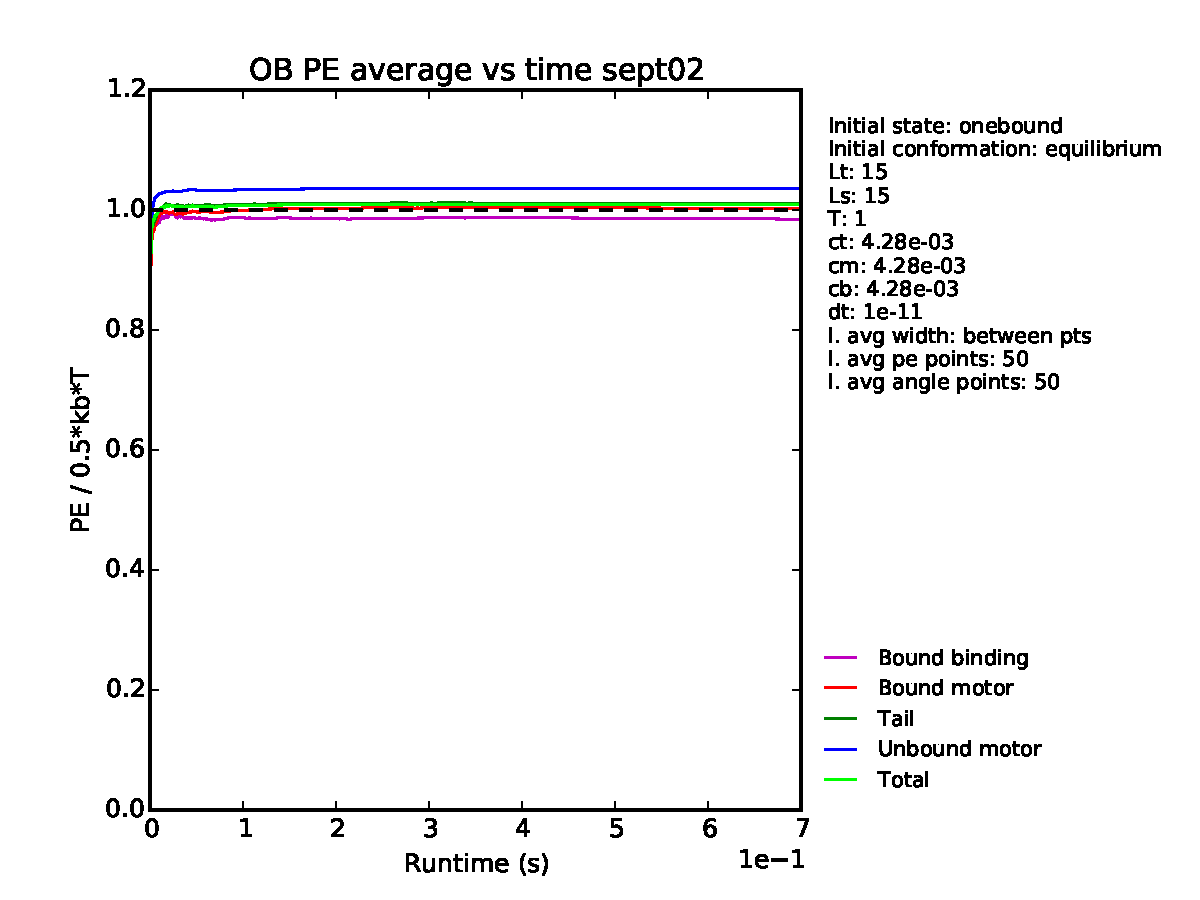
\includegraphics[width=\textwidth]{../../figures/OB_Average_PE.pdf}
    \caption{Onebound average spring energy.}{Average domain PE of onebound model converging to $\frac12 k_BT$ energy over time.}
  \end{minipage}
  \hspace{.2cm}
  \begin{minipage}[b]{0.45\textwidth}
    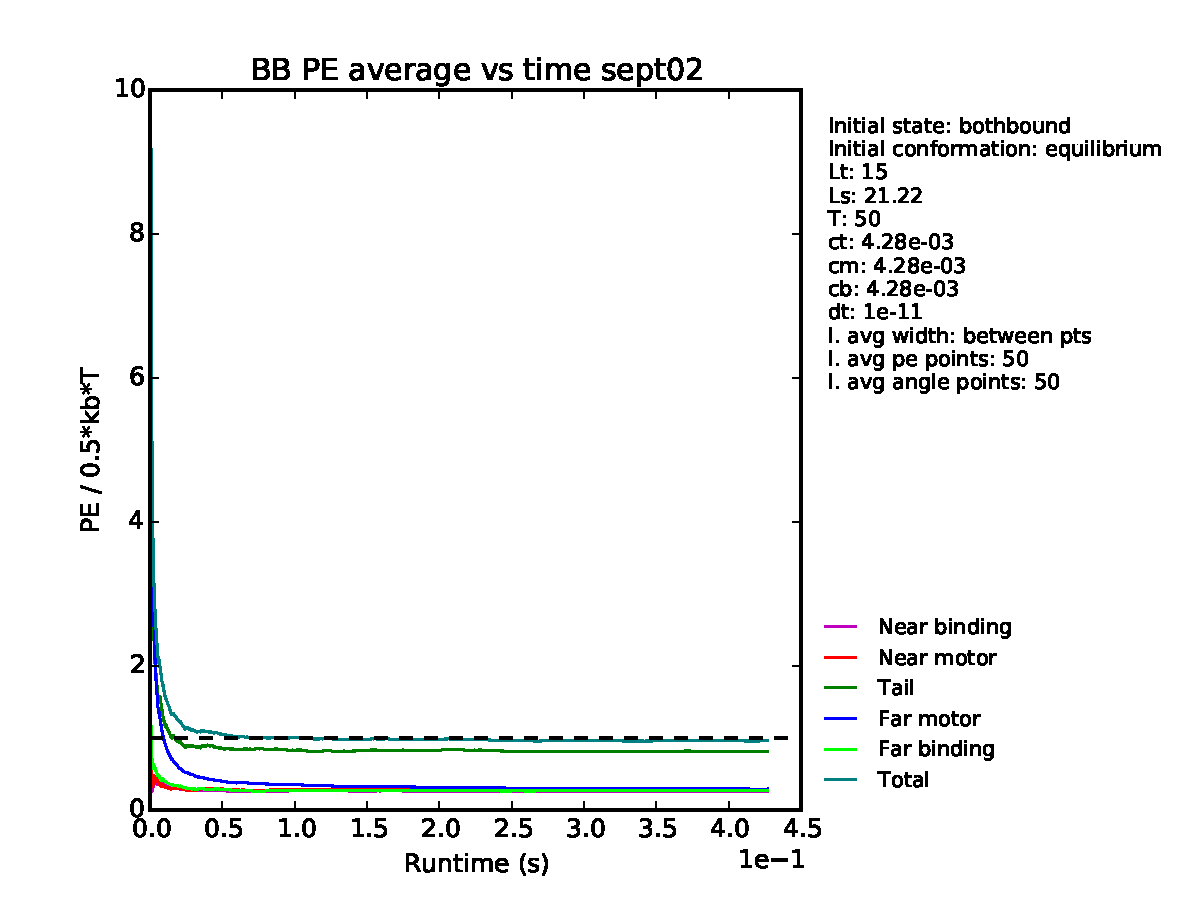
\includegraphics[width=\textwidth]{../../figures/BB_Average_PE.pdf}
    \caption{Bothbound average spring energy.}{Total domain PE of bothbound model converging to $\frac12 k_BT$ energy over time.}
  \end{minipage}
  \label{fig:equipartition_agreement}
\end{figure}

\textbf{would it be a stronger test to also calculate the standard deviation of <PE>? It seems like <PE> would still equal N/2KbT as long as the forces/velocities were symmetrically wrong. Calculating the stdev would require the state occupation to actually the ET. Or, maybe just plot the angle occupation and show that it is what it should be?}

\textbf{Possibly do mutations on motion equations to show that tests are no longer behaved}

\begin{figure}[h]
  \centering
  \begin{tabular}{| c | c | c | c |}
    \hline
    Author & Conditions & Velocity & Run length\\\hline
    Qiu \cite{weihongpaper} & 1mM [ATP] & $134 \pm 60.4$ nm & $1.06 \pm 0.044 \mu m$\\ \hline
    Reck-Peterson \cite{reck2006single} & 1mM [ATP] & $85 \pm 30 nm/s$  & $1.9 \pm 0.2 \mu m$\\ \hline
  \end{tabular}
  \caption{Literature values for experimental dynein stepping behavior.}{Table of literature values for dynein behavior}
  \label{table:parameter-table}
\end{figure}

%% \subsection{Data collection}
%% Time evolution of the system has the potential to create a huge amount of data, so care has to be taken to only collect what is necessary. For the purposes of testing stepping behavior of the model the geometry and per-domain forces and energies can be safely ignored. All that is needed to determine model fitness is the size and duration of each step.\\

%% \subsubsection{Stepping data output and calculation}
%% A step is defined as a complete cycle of 

%% \subsubsection{Simulation running via SLURM}

\subsection{Parameter fitting}
There are 14 free variables in the dynein model: rigid rod lengths $L_s$ and $L_t$, domain radii $R_b$, $R_m$ and $R_t$, spring constants $c_b$, $c_m$ and $c_t$, equilibrium angles $\theta_{b,eq}$, $\theta_{t,eq}$, $\Theta_{m,eq}^{Pre}$, $\Theta_{m,eq}^{Post}$, onebound binding rate $k_b$, and bothbound unbinding rate $k_{ub}$. Some of these values are found easily from literature or by looking at crystal structures of the motor protein, as shown in Table \ref{parameter-table}.\\

Others are more difficult to find. These values, including $k_b$, $k_ub$ and the three spring constants, are fit by an optimization process. First un/binding rates are fit to one/bothbound times, then spring constants are fit to average step length. This process is chronicled below.

\begin{figure}[h]
  \centering
  \begin{tabular}{| l | l | l | l | l | l | l | l | l |}
    \hline
    & Winch (Sarlah) & Schmidt & Lin & PyMol 3VKH & PyMol 4RH7 & Redwine & Kon & Burgess \\\hline
    $L_s$ & 12nm & & & 21.0nm & 22.1nm & & & \\ \hline
    $L_t$ &  7nm & & & & 11.15nm & & & \\ \hline
    $R_b$ &  & & & 1.57nm & 1.45nm & & & \\ \hline
    $R_m$ &  7nm & & & 7.36nm & 6.3nm & & & \\ \hline
    $R_t$ &  & & & & 2.16nm & & & \\ \hline
    $\theta_{m}^{Pre}$ & 250$^{\circ}$ & & 171$^{\circ}$ & & & & & 160\\ \hline
    $\theta_{m}^{Post}$ & 330$^{\circ}$ & & 137.5$^{\circ}$ & & & & & 136\\ \hline
    $\theta_{b}$ & 56$^{\circ}$ & & 63.5$^{\circ}$ & & & & & \\ \hline
    $\theta_{t}$ & 0$^{\circ}$ & & & & & & & \\ \hline
    $k_{ub}$ & $180 s^{-1,a}$ & & & & & & $90.2 \pm 4.5$& \\ \hline
    $k_b$ & $460 s^{-1,b}$ & & & & & & & \\ \hline
    $c_t$ & & & & & & & & \\ \hline
    $c_m$ & & & & & & & & \\ \hline
    $c_b$ & & & & & & 140 kJ/mol & & \\ \hline
  \end{tabular}
  \caption{Literature values for dynein model parameters.}{Table of literature values for various free parameters in dynein model.}
  \label{table:parameter-table}
\end{figure}

In addition, the physical conditions the simulations were run at are shown in Table \ref{table:simulation-conditions}. These conditions are meant to reflect the conditions found inside a typical cell. \textbf{of what species?}\\

\begin{figure}[h]
  \centering
  \begin{tabular}{| l | l |}
    \hline
    T & [ATP] \\ \hline
    310.15 K & $1mM$\\ \hline
  \end{tabular}
  \caption{Physical constants of simulation.}{Table of physical constants used in simulation.}
  \label{table:simulation-std-conditions}
\end{figure}

\subsubsection{Fitting rate constants}
To find the ideal binding and unbinding rates of our model, we ran simulations at various $k_b$ and $k_{ub}$ conditions. The time each simulation spent in each state, $t_{bb}$ and $t_{ob}$, was compared with the experimental data shown in Table \ref{table:time-parameter-table}. Simulation behavior for a wide range of $k_b$ and $k_{ub}$ values is shown as a heat map in Figure \ref{fig:kb-kub-heatmap}.\\

\begin{figure}[H]
  \centering
  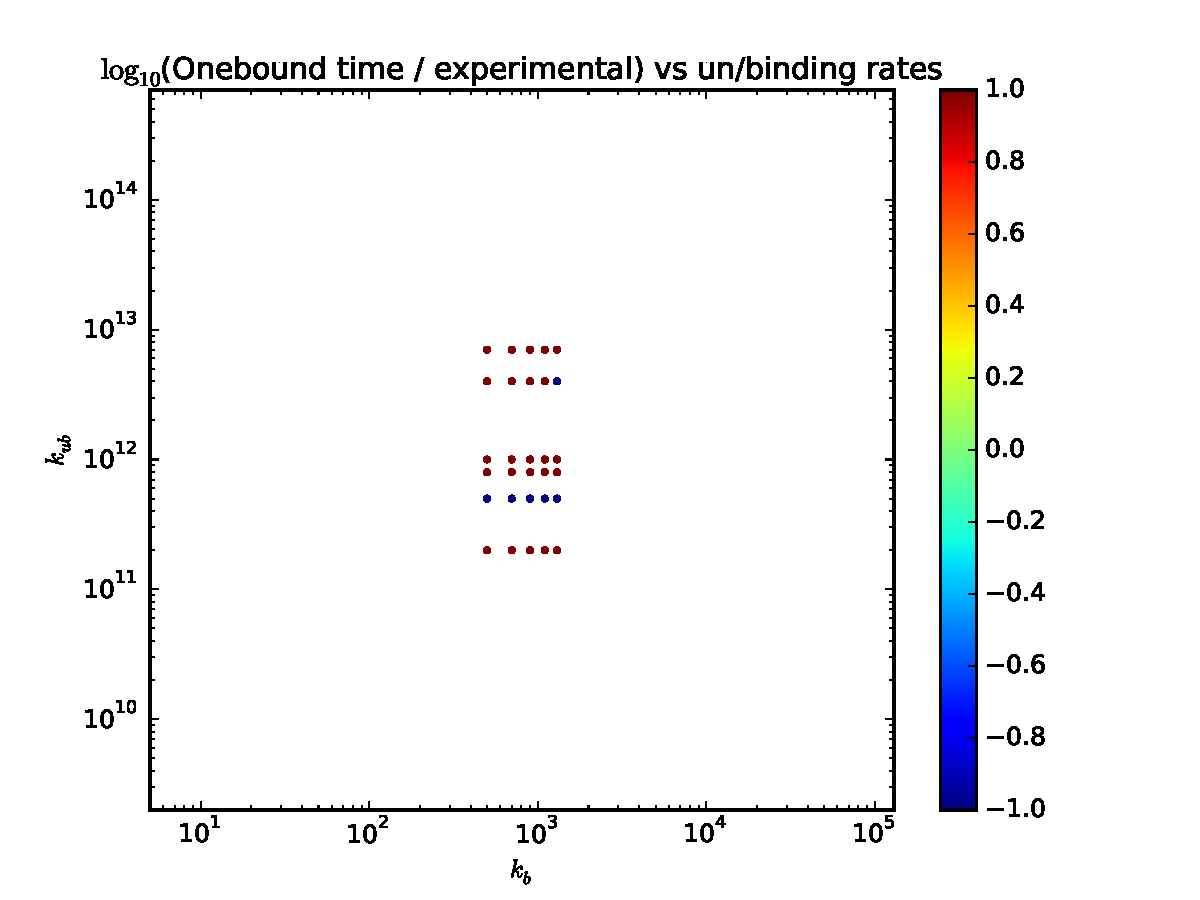
\includegraphics[width=\textwidth]{../../figures/kb-kub-contour}
  \caption{Heat map comparing $k_b$ and $k_{ub}$ values to time spent in the onebound state. Simulations run for XXXXX seconds at standard conditions shown in Table \ref{table:simulation-std-conditions}, with spring constants $c_b = c_m = c_t = 2.4\Delta G_{ATP}$, $L_s=22.1nm$ and $L_t=11.15nm$.}
  \label{fig:kb-kub-heatmap}
\end{figure}

\subsubsection{Fitting spring constants}
This section will be written once it is conducted. This is contingent on getting rate fitting done, and preferably high-dt simulations stable so an optimization process can be run.\\

\section{Chapter: Results}
The ideal set of parameters found via the fitting process is shown in Table \ref{table:final-parameter-table}.\\

\begin{figure}[H]
  \centering
  \begin{tabular}{| l | l | l | l | l | l | l | l | l | l | l | l | l | l | l |}
    \hline
    $L_s$ & $L_t$ & $R_b$ & $R_m$ & $R_t$ & $\theta_{m}^{Pre}$ & $\theta_{m}^{Post}$ & $\theta_{b}$ & $\theta_{t}$ & $A_{ub}$ & $A_b$ & $c_t$ & $c_m$  &$c_b$\\ \hline
    21.0nm & 11.15nm & 1.45nm & 6.3nm & 2.2nm & 136$^{\circ}$ & 171$^{\circ}$ & 63.5$^{\circ}$ & 0$^{\circ}$ &  &  &  &   & \\ \hline
  \end{tabular}
  \caption{Ideal parameters for model stepping.}{Table of ideal parameters for reproducing \textit{in vivo} dynein stepping behavior.}
  \label{table:final-parameter-table}
\end{figure}

Histograms of the simulation's stepping length and time are shown in Figure \ref{fig:final-histograms}. This figure also shows histograms for experimental dynein stepping behavior.\\

\begin{figure}[H]
  \centering
  \begin{minipage}[b]{0.45\textwidth}
    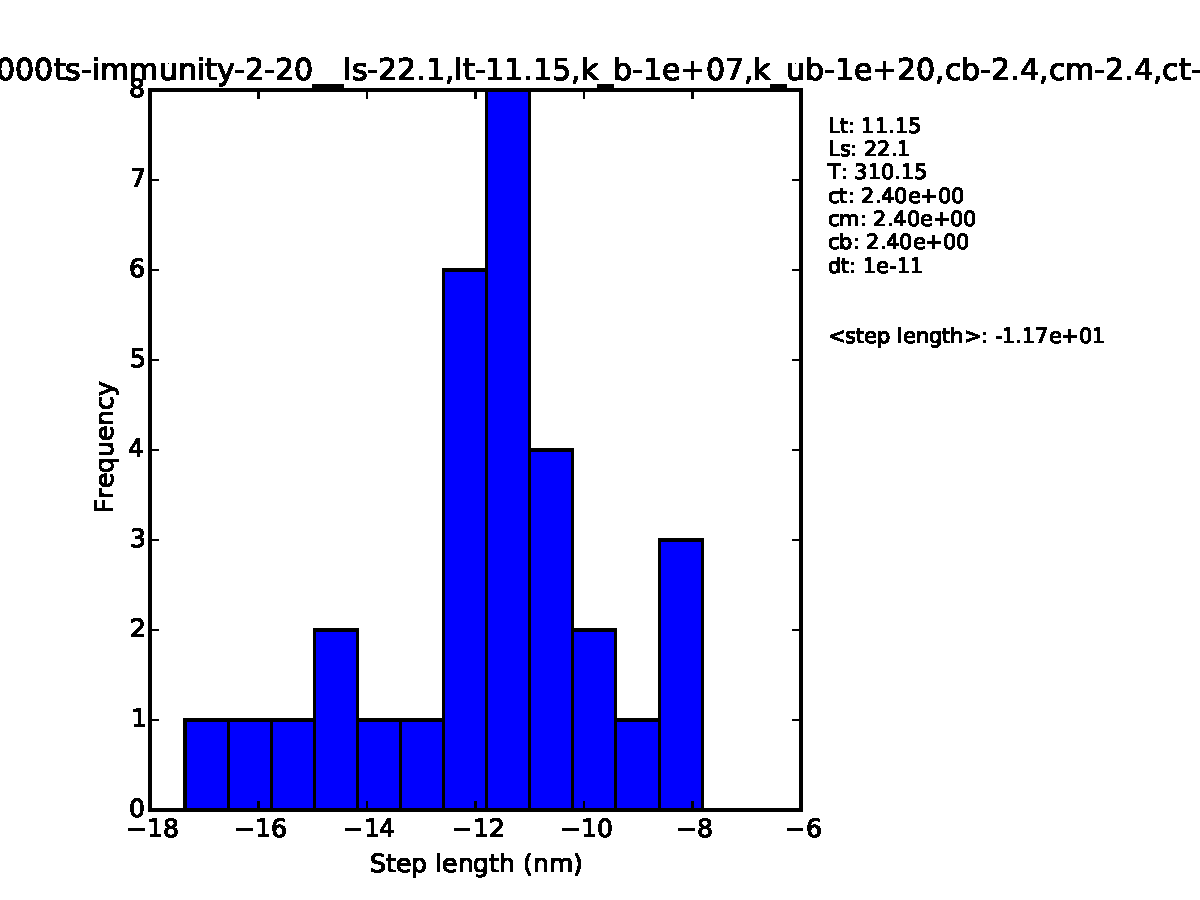
\includegraphics[width=\textwidth]{../../figures/length_histogram_sample.pdf}
    \caption{Histogram of simulated stepping lengths using ideal dynein parameters. Todo: make these figures compare better.}
  \end{minipage}
  \hspace{.1cm}
  \begin{minipage}[b]{0.45\textwidth}
    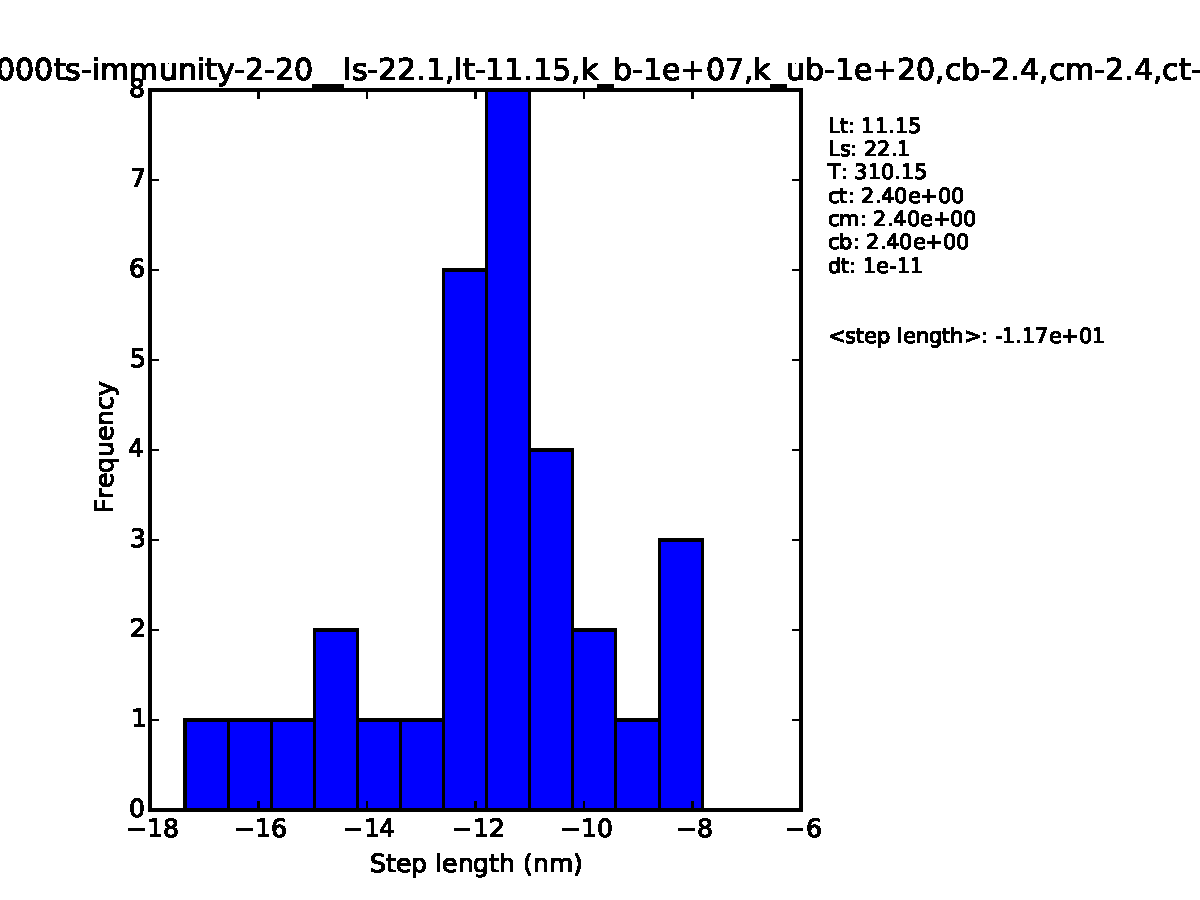
\includegraphics[width=\textwidth]{../../figures/time_histogram_sample.pdf}
    \caption{Histogram of simulated stepping times using ideal dynein parameters.}
  \end{minipage}\\
  \begin{minipage}[b]{0.45\textwidth}
    \includegraphics[width=\textwidth]{../../figures/weihong-step-size.pdf}
    \caption{Experimental dynein step size from \cite{weihongpaper}.}
  \end{minipage}
  \hspace{.1cm}
  \begin{minipage}[b]{0.45\textwidth}
    \includegraphics[width=\textwidth]{../../figures/weihong-velocity.pdf}
    \caption{Experimental dynein step time from \cite{weihongpaper}}
  \end{minipage}
  \label{fig:final-histograms}
\end{figure}

\section{Chapter: Discussion}
\subsubsection{Limitations}
The accuracy of correspondence between model dynein and physical dynein is very relevant when assessing the meaningfulness of the simulation results. Reducing a megaDalton weight protein to a five-coordinate kinematic model with springy hinges is bound to have low resolution. However, the point of this model is to predict gross stepping behavior over large timescales. Thus, only assumptions which possibly add large systematic errors to stepping behavior are of interest. These possible limitations are listed below.\\

\paragraph{Spherical domains}
Domain shape influences primarily the drag coefficients $\gamma$ of the model. These in turn affect the diffusion rate of different domains. Reducing domains to spheres adds a systematic error to the diffusion speed of each domain, which could bias step size. However, spring constants $c_b$, $c_m$ and $c_t$ also have an influence on the diffusion rate of spheres. Thus by fitting spring constants to the proper step length, the systematic error of domain size can be reduced -- ???\\

-------------------------------------
Talk about the things we \textit{don't} take into account...motor-motor interaction, 2d information, other ATPase nucleotide state, saying certain mechanochemical steps occur ``fast,'' not taking into account all mechanochemical cycle states, making the coiled coil domain rigid even though it may be springy...

Mention the Burgess paper, which says spring constants might change between apo/ADP states.
Also dynein may move helically: Bidirectional helical motility of cytoplasmic dynein around microtubules

Computational limitations: Our project is computational, not experimental. Thus the onus is on us to show that our system is not a humongously over-fit model which just happens to reproduce experimental data, but rather a good physical model of dynein which also replicates data.\\
-------------------------------------

\subsection{Future work on this project}
If setbacks happen, this'll be a big section. Or, further simulations which could be done. Namely taking our model and giving it lots more states and seeing if this model even better fits experimental data.\\

\subsubsection{Experiments to verify our model}
Talk about how FRET could be used to verify our model. We have domain distance info over long
timescales in our model - this is something we could compare to a FRET experiment exploring
the distance between domains in dynein.\\

Other biophysics experiments which could verify our model?\\

Do our spring constants seem to indicate that the protein does about one ATP's worth of work through its cycle? I wonder if the motor cools down its surroundings when it walks...\\

Calorimetry could get Gibb's energy of binding if you froze the motor in onebound using
vanadium? Maybe...\\
\subsection{Possible further projects}
\subsection{Difference between dynein and kinesin}
Our project un/successfully predicted how dynein behaved. How would we modify it to describe kinesin?
Is dynein's linker-motor connection less tense than kinesin's, leading to more random motion? This
would likely be lots of speculation, but it could be cool to look up some papers on kinesin motility
and get its crystal structure to do some comparisons.

\bibliography{thesis-articles}

%% \bibliography{thesis-webpages}

\section{Appendix}

\subsubsection{Glossary}
\textbf{ATP} Adenosine triphosphate is a small organic molecule which very spontaneously breaks apart into ADP and a phosphate. This reaction is used to power many energy-requiring mechanisms within the cell. This reaction has a $\Delta G^\circ \approx -36 kJ/mol$ at physiological conditions \ref{ATPenergy}.\\\\
\textbf{Protein} Dynein is a protein, or long chain of amino acids linked together and folded into a particular shape.\\

\subsection{Motion equations}

\subsubsection{Onebound equations}
\label{sec:ob-motion-equations}
The following is a continuation of the derivation for the full motion equations used to time evolve the onebound model:

\begin{align*}
AA &= L_s\sin\theta_{bb}      &   LL &= -L_s\cos(\theta_{bb})\\
BB &= L_t\sin(\theta_{bm})    &	 MM &= -L_t\cos(\theta_{bm})\\
CC &= -L_t\sin(\theta_{um})   &	 NN &= L_t\cos(\theta_{um})\\
DD &= -L_s\sin(\theta_{ub})   &	 OO &= L_s\cos(\theta_{ub})\\
\\
EE &= -\gamma_m (X_{bm} - X_{bb})       &  PP &= -\gamma_m (Y_{bm} - Y_{bb})\\
FF &= \gamma_m (X_{t } - X_{bm})        &	 QQ &= \gamma_m (Y_{t } - Y_{bm})\\ 
GG &= -\gamma_t (X_{t } - X_{bm})       &	 RR &= -\gamma_t (Y_{t } - Y_{bm})\\
HH &= \gamma_t (X_{um} - X_{t })        &	 SS &= \gamma_t (Y_{um} - Y_{t })\\ 
II &= -\gamma_m (X_{um} - X_{t })       &	 TT &= -\gamma_m (Y_{um} - Y_{t })\\
JJ &= \gamma_m (X_{ub} - X_{um})        &	 UU &= \gamma_m (Y_{ub} - Y_{um})\\ 
KK &= -\gamma_b (X_{ub} - X_{um})       &	 VV &= -\gamma_b (Y_{ub} - Y_{um})\\
\end{align*}%
%
\[
\begin{pmatrix}
  AA & 0 & 0 & 0 & EE & FF & 0 & 0\\
  AA & BB & 0 & 0 & 0 & GG & HH & 0\\
  AA & BB & CC & 0 & 0 & 0 & II & JJ\\
  AA & BB & CC & DD & 0 & 0 & 0 & KK\\
  LL & 0 & 0 & 0 & PP & QQ & 0 & 0\\
  LL & MM & 0 & 0 & 0 & RR & SS & 0\\
  LL & MM & NN & 0 & 0 & 0 & TT & UU\\
  LL & MM & NN & OO & 0 & 0 & 0 & VV\\
\end{pmatrix}
\begin{pmatrix}
    \dot{\theta}_{bb}\\
    \dot{\theta}_{bm}\\
    \dot{\theta}_{um}\\
    \dot{\theta}_{ub}\\
    \lambda_{bs}\\
    \lambda_{bt}\\
    \lambda_{ut}\\
    \lambda_{us}\\
  \end{pmatrix}
=
\begin{pmatrix}
  X1\\
  X2\\
  X3\\
  X4\\
  X5\\
  X6\\
  X7\\
  X8\\
\end{pmatrix}
\]

Solving the above system for $\dot{\Theta}_{bb}, \dot{\Theta}_{bm}, \dot{\Theta}_{um}$ and $\dot{\Theta}_{ub}$ gives the desired velocities. Solution was done via Mathematica.

%% $\dot{\Theta}_{bb}$ =
%% {\tiny
%% ( - (GG*II*MM*NN*PP*X1) + CC*HH*MM*PP*RR*X1 - BB*HH*NN*PP*RR*X1 + BB*II*NN*PP*RR*X1 - CC*GG*MM*PP*SS*X1 + BB*GG*NN*PP*SS*X1 + CC*GG*MM*PP*TT*X1 - BB*CC*PP*RR*TT*X1 + FF*II*MM*NN*PP*X2 - EE*II*MM*NN*QQ*X2 + CC*FF*MM*PP*SS*X2 - BB*FF*NN*PP*SS*X2 - CC*EE*MM*QQ*SS*X2 + BB*EE*NN*QQ*SS*X2 - CC*FF*MM*PP*TT*X2 + CC*EE*MM*QQ*TT*X2 - FF*HH*MM*NN*PP*X3 + EE*HH*MM*NN*QQ*X3 + BB*FF*NN*PP*SS*X3 - BB*EE*NN*QQ*SS*X3 + EE*GG*II*MM*NN*X5 - CC*EE*HH*MM*RR*X5 + BB*EE*HH*NN*RR*X5 - BB*EE*II*NN*RR*X5 + CC*EE*GG*MM*SS*X5 - BB*EE*GG*NN*SS*X5 - CC*EE*GG*MM*TT*X5 + BB*CC*EE*RR*TT*X5 - CC*FF*HH*MM*PP*X6 + BB*FF*HH*NN*PP*X6 - BB*FF*II*NN*PP*X6 + CC*EE*HH*MM*QQ*X6 - BB*EE*HH*NN*QQ*X6 + BB*EE*II*NN*QQ*X6 + BB*CC*FF*PP*TT*X6 - BB*CC*EE*QQ*TT*X6 + CC*FF*HH*MM*PP*X7 - CC*EE*HH*MM*QQ*X7 - BB*CC*FF*PP*SS*X7 + BB*CC*EE*QQ*SS*X7)/(EE*GG*II*LL*MM*NN + BB*FF*HH*LL*NN*PP - BB*FF*II*LL*NN*PP - AA*FF*HH*MM*NN*PP + AA*FF*II*MM*NN*PP - AA*GG*II*MM*NN*PP - BB*EE*HH*LL*NN*QQ + BB*EE*II*LL*NN*QQ + AA*EE*HH*MM*NN*QQ - AA*EE*II*MM*NN*QQ - CC*EE*HH*LL*MM*RR + BB*EE*HH*LL*NN*RR - BB*EE*II*LL*NN*RR + AA*CC*HH*MM*PP*RR - AA*BB*HH*NN*PP*RR + AA*BB*II*NN*PP*RR + CC*EE*GG*LL*MM*SS - BB*EE*GG*LL*NN*SS - BB*CC*FF*LL*PP*SS + AA*CC*FF*MM*PP*SS - AA*CC*GG*MM*PP*SS + AA*BB*GG*NN*PP*SS + BB*CC*EE*LL*QQ*SS - AA*CC*EE*MM*QQ*SS - CC*EE*GG*LL*MM*TT + BB*CC*FF*LL*PP*TT - AA*CC*FF*MM*PP*TT + AA*CC*GG*MM*PP*TT - BB*CC*EE*LL*QQ*TT + AA*CC*EE*MM*QQ*TT + BB*CC*EE*LL*RR*TT - AA*BB*CC*PP*RR*TT) - ((FF*PP - EE*QQ)*(HH*MM - BB*SS)*(JJ*NN - CC*UU)*( - ((( Power(AA,6)* Power(BB,2)*CC*DD*HH*MM -  Power(AA,6)* Power(BB,3)*DD*HH*NN +  Power(AA,6)* Power(BB,3)*DD*II*NN -  Power(AA,6)* Power(BB,3)*CC*II*OO)*( - (EE*LL) + AA*PP)*( - (( Power(AA,3)* Power(BB,2)*CC*EE*LL -  Power(AA,4)*BB*CC*EE*MM)*( - (FF*LL) + AA*QQ)) + ( - (EE*LL) + AA*PP)*( Power(AA,4)*BB*CC*GG*MM -  Power(AA,2)*BB*CC*( - (AA*BB*FF*LL) +  Power(AA,2)*FF*MM +  Power(AA,2)*BB*RR))) - ( - (EE*LL) + AA*PP)*(( Power(AA,5)* Power(BB,3)*CC*DD*FF*LL -  Power(AA,6)* Power(BB,2)*CC*DD*FF*MM +  Power(AA,6)* Power(BB,2)*CC*DD*GG*MM -  Power(AA,6)* Power(BB,3)*DD*GG*NN)*( - (EE*LL) + AA*PP) - ( Power(AA,5)* Power(BB,3)*CC*DD*EE*LL -  Power(AA,6)* Power(BB,2)*CC*DD*EE*MM)*( - (FF*LL) + AA*QQ))*( Power(AA,4)*BB*CC*HH*MM -  Power(AA,4)* Power(BB,2)*CC*SS))*( - ((( Power(AA,3)* Power(BB,2)*CC*FF*LL -  Power(AA,4)*BB*CC*FF*MM +  Power(AA,4)*BB*CC*GG*MM -  Power(AA,4)* Power(BB,2)*GG*NN)*( - (EE*LL) + AA*PP) - ( Power(AA,3)* Power(BB,2)*CC*EE*LL -  Power(AA,4)*BB*CC*EE*MM)*( - (FF*LL) + AA*QQ))*( - (( Power(AA,3)* Power(BB,2)*CC*EE*LL -  Power(AA,4)*BB*CC*EE*MM)*( - (LL*X1) + AA*X5)) + ( - (EE*LL) + AA*PP)*( Power(AA,3)* Power(BB,2)*CC*LL*X1 -  Power(AA,4)*BB*CC*MM*X1 +  Power(AA,4)*BB*CC*MM*X2 -  Power(AA,4)* Power(BB,2)*CC*X6))) + ( - (( Power(AA,3)* Power(BB,2)*CC*EE*LL -  Power(AA,4)*BB*CC*EE*MM)*( - (FF*LL) + AA*QQ)) + ( - (EE*LL) + AA*PP)*( Power(AA,4)*BB*CC*GG*MM -  Power(AA,2)*BB*CC*( - (AA*BB*FF*LL) +  Power(AA,2)*FF*MM +  Power(AA,2)*BB*RR)))*( - (( Power(AA,3)* Power(BB,2)*CC*EE*LL -  Power(AA,4)*BB*CC*EE*MM)*( - (LL*X1) + AA*X5)) + ( - (EE*LL) + AA*PP)*( Power(AA,3)* Power(BB,2)*CC*LL*X1 -  Power(AA,4)*BB*CC*MM*X1 +  Power(AA,4)*BB*CC*MM*X2 -  Power(AA,4)* Power(BB,2)*NN*X2 +  Power(AA,4)* Power(BB,2)*NN*X3 -  Power(AA,4)* Power(BB,2)*CC*X7)))) + ( - (( - (EE*LL) + AA*PP)*(( Power(AA,3)* Power(BB,2)*CC*FF*LL -  Power(AA,4)*BB*CC*FF*MM +  Power(AA,4)*BB*CC*GG*MM -  Power(AA,4)* Power(BB,2)*GG*NN)*( - (EE*LL) + AA*PP) - ( Power(AA,3)* Power(BB,2)*CC*EE*LL -  Power(AA,4)*BB*CC*EE*MM)*( - (FF*LL) + AA*QQ))*( Power(AA,4)*BB*CC*HH*MM -  Power(AA,4)* Power(BB,2)*CC*SS)) + ( - (EE*LL) + AA*PP)*( - (( Power(AA,3)* Power(BB,2)*CC*EE*LL -  Power(AA,4)*BB*CC*EE*MM)*( - (FF*LL) + AA*QQ)) + ( - (EE*LL) + AA*PP)*( Power(AA,4)*BB*CC*GG*MM -  Power(AA,2)*BB*CC*( - (AA*BB*FF*LL) +  Power(AA,2)*FF*MM +  Power(AA,2)*BB*RR)))*( Power(AA,4)*BB*CC*HH*MM -  Power(AA,4)* Power(BB,2)*HH*NN +  Power(AA,4)* Power(BB,2)*II*NN -  Power(AA,4)* Power(BB,2)*CC*TT))*( - ((( Power(AA,5)* Power(BB,3)*CC*DD*FF*LL -  Power(AA,6)* Power(BB,2)*CC*DD*FF*MM +  Power(AA,6)* Power(BB,2)*CC*DD*GG*MM -  Power(AA,6)* Power(BB,3)*DD*GG*NN)*( - (EE*LL) + AA*PP) - ( Power(AA,5)* Power(BB,3)*CC*DD*EE*LL -  Power(AA,6)* Power(BB,2)*CC*DD*EE*MM)*( - (FF*LL) + AA*QQ))*( - (( Power(AA,3)* Power(BB,2)*CC*EE*LL -  Power(AA,4)*BB*CC*EE*MM)*( - (LL*X1) + AA*X5)) + ( - (EE*LL) + AA*PP)*( Power(AA,3)* Power(BB,2)*CC*LL*X1 -  Power(AA,4)*BB*CC*MM*X1 +  Power(AA,4)*BB*CC*MM*X2 -  Power(AA,4)* Power(BB,2)*CC*X6))) + ( - (( Power(AA,3)* Power(BB,2)*CC*EE*LL -  Power(AA,4)*BB*CC*EE*MM)*( - (FF*LL) + AA*QQ)) + ( - (EE*LL) + AA*PP)*( Power(AA,4)*BB*CC*GG*MM -  Power(AA,2)*BB*CC*( - (AA*BB*FF*LL) +  Power(AA,2)*FF*MM +  Power(AA,2)*BB*RR)))*( - (( Power(AA,5)* Power(BB,3)*CC*DD*EE*LL -  Power(AA,6)* Power(BB,2)*CC*DD*EE*MM)*( - (LL*X1) + AA*X5)) + ( - (EE*LL) + AA*PP)*( Power(AA,5)* Power(BB,3)*CC*DD*LL*X1 -  Power(AA,6)* Power(BB,2)*CC*DD*MM*X1 +  Power(AA,6)* Power(BB,2)*CC*DD*MM*X2 -  Power(AA,6)* Power(BB,3)*DD*NN*X2 +  Power(AA,6)* Power(BB,3)*DD*NN*X3 -  Power(AA,6)* Power(BB,3)*CC*OO*X3 +  Power(AA,6)* Power(BB,3)*CC*OO*X4 -  Power(AA,6)* Power(BB,3)*CC*DD*X8)))))/(( - (EE*GG*II*LL*MM*NN) - BB*FF*HH*LL*NN*PP + BB*FF*II*LL*NN*PP + AA*FF*HH*MM*NN*PP - AA*FF*II*MM*NN*PP + AA*GG*II*MM*NN*PP + BB*EE*HH*LL*NN*QQ - BB*EE*II*LL*NN*QQ - AA*EE*HH*MM*NN*QQ + AA*EE*II*MM*NN*QQ + CC*EE*HH*LL*MM*RR - BB*EE*HH*LL*NN*RR + BB*EE*II*LL*NN*RR - AA*CC*HH*MM*PP*RR + AA*BB*HH*NN*PP*RR - AA*BB*II*NN*PP*RR - CC*EE*GG*LL*MM*SS + BB*EE*GG*LL*NN*SS + BB*CC*FF*LL*PP*SS - AA*CC*FF*MM*PP*SS + AA*CC*GG*MM*PP*SS - AA*BB*GG*NN*PP*SS - BB*CC*EE*LL*QQ*SS + AA*CC*EE*MM*QQ*SS + CC*EE*GG*LL*MM*TT - BB*CC*FF*LL*PP*TT + AA*CC*FF*MM*PP*TT - AA*CC*GG*MM*PP*TT + BB*CC*EE*LL*QQ*TT - AA*CC*EE*MM*QQ*TT - BB*CC*EE*LL*RR*TT + AA*BB*CC*PP*RR*TT)*( - (( - (EE*LL) + AA*PP)*( - (( Power(AA,3)* Power(BB,2)*CC*EE*LL -  Power(AA,4)*BB*CC*EE*MM)*( - (FF*LL) + AA*QQ)) + ( - (EE*LL) + AA*PP)*( Power(AA,4)*BB*CC*GG*MM -  Power(AA,2)*BB*CC*( - (AA*BB*FF*LL) +  Power(AA,2)*FF*MM +  Power(AA,2)*BB*RR)))*(( Power(AA,6)* Power(BB,2)*CC*DD*HH*MM -  Power(AA,6)* Power(BB,3)*DD*HH*NN +  Power(AA,6)* Power(BB,3)*DD*II*NN -  Power(AA,6)* Power(BB,3)*CC*II*OO)*( - (EE*LL) + AA*PP)*( - (( Power(AA,3)* Power(BB,2)*CC*EE*LL -  Power(AA,4)*BB*CC*EE*MM)*( - (FF*LL) + AA*QQ)) + ( - (EE*LL) + AA*PP)*( Power(AA,4)*BB*CC*GG*MM -  Power(AA,2)*BB*CC*( - (AA*BB*FF*LL) +  Power(AA,2)*FF*MM +  Power(AA,2)*BB*RR))) - ( - (EE*LL) + AA*PP)*(( Power(AA,5)* Power(BB,3)*CC*DD*FF*LL -  Power(AA,6)* Power(BB,2)*CC*DD*FF*MM +  Power(AA,6)* Power(BB,2)*CC*DD*GG*MM -  Power(AA,6)* Power(BB,3)*DD*GG*NN)*( - (EE*LL) + AA*PP) - ( Power(AA,5)* Power(BB,3)*CC*DD*EE*LL -  Power(AA,6)* Power(BB,2)*CC*DD*EE*MM)*( - (FF*LL) + AA*QQ))*( Power(AA,4)*BB*CC*HH*MM -  Power(AA,4)* Power(BB,2)*CC*SS))*( Power(AA,4)* Power(BB,2)*JJ*NN -  Power(AA,4)* Power(BB,2)*CC*UU)) + ( - (EE*LL) + AA*PP)*( - (( Power(AA,3)* Power(BB,2)*CC*EE*LL -  Power(AA,4)*BB*CC*EE*MM)*( - (FF*LL) + AA*QQ)) + ( - (EE*LL) + AA*PP)*( Power(AA,4)*BB*CC*GG*MM -  Power(AA,2)*BB*CC*( - (AA*BB*FF*LL) +  Power(AA,2)*FF*MM +  Power(AA,2)*BB*RR)))*( - (( - (EE*LL) + AA*PP)*(( Power(AA,3)* Power(BB,2)*CC*FF*LL -  Power(AA,4)*BB*CC*FF*MM +  Power(AA,4)*BB*CC*GG*MM -  Power(AA,4)* Power(BB,2)*GG*NN)*( - (EE*LL) + AA*PP) - ( Power(AA,3)* Power(BB,2)*CC*EE*LL -  Power(AA,4)*BB*CC*EE*MM)*( - (FF*LL) + AA*QQ))*( Power(AA,4)*BB*CC*HH*MM -  Power(AA,4)* Power(BB,2)*CC*SS)) + ( - (EE*LL) + AA*PP)*( - (( Power(AA,3)* Power(BB,2)*CC*EE*LL -  Power(AA,4)*BB*CC*EE*MM)*( - (FF*LL) + AA*QQ)) + ( - (EE*LL) + AA*PP)*( Power(AA,4)*BB*CC*GG*MM -  Power(AA,2)*BB*CC*( - (AA*BB*FF*LL) +  Power(AA,2)*FF*MM +  Power(AA,2)*BB*RR)))*( Power(AA,4)*BB*CC*HH*MM -  Power(AA,4)* Power(BB,2)*HH*NN +  Power(AA,4)* Power(BB,2)*II*NN -  Power(AA,4)* Power(BB,2)*CC*TT))*( Power(AA,6)* Power(BB,3)*DD*JJ*NN -  Power(AA,6)* Power(BB,3)*CC*JJ*OO +  Power(AA,6)* Power(BB,3)*CC*KK*OO -  Power(AA,6)* Power(BB,3)*CC*DD*VV)))
%% } \break

%% $\dot{\Theta}_{bm}$ =
%% {\tiny
%%   (GG*II*LL*NN*PP*X1 - CC*HH*LL*PP*RR*X1 + AA*HH*NN*PP*RR*X1 - AA*II*NN*PP*RR*X1 + CC*GG*LL*PP*SS*X1 - AA*GG*NN*PP*SS*X1 - CC*GG*LL*PP*TT*X1 + AA*CC*PP*RR*TT*X1 - FF*II*LL*NN*PP*X2 + EE*II*LL*NN*QQ*X2 - EE*II*LL*NN*RR*X2 + AA*II*NN*PP*RR*X2 - CC*FF*LL*PP*SS*X2 + AA*FF*NN*PP*SS*X2 + CC*EE*LL*QQ*SS*X2 - AA*EE*NN*QQ*SS*X2 + CC*FF*LL*PP*TT*X2 - CC*EE*LL*QQ*TT*X2 + CC*EE*LL*RR*TT*X2 - AA*CC*PP*RR*TT*X2 + FF*HH*LL*NN*PP*X3 - EE*HH*LL*NN*QQ*X3 + EE*HH*LL*NN*RR*X3 - AA*HH*NN*PP*RR*X3 - EE*GG*LL*NN*SS*X3 - AA*FF*NN*PP*SS*X3 + AA*GG*NN*PP*SS*X3 + AA*EE*NN*QQ*SS*X3 - EE*GG*II*LL*NN*X5 + CC*EE*HH*LL*RR*X5 - AA*EE*HH*NN*RR*X5 + AA*EE*II*NN*RR*X5 - CC*EE*GG*LL*SS*X5 + AA*EE*GG*NN*SS*X5 + CC*EE*GG*LL*TT*X5 - AA*CC*EE*RR*TT*X5 + EE*GG*II*LL*NN*X6 + CC*FF*HH*LL*PP*X6 - AA*FF*HH*NN*PP*X6 + AA*FF*II*NN*PP*X6 - AA*GG*II*NN*PP*X6 - CC*EE*HH*LL*QQ*X6 + AA*EE*HH*NN*QQ*X6 - AA*EE*II*NN*QQ*X6 - CC*EE*GG*LL*TT*X6 - AA*CC*FF*PP*TT*X6 + AA*CC*GG*PP*TT*X6 + AA*CC*EE*QQ*TT*X6 - CC*FF*HH*LL*PP*X7 + CC*EE*HH*LL*QQ*X7 - CC*EE*HH*LL*RR*X7 + AA*CC*HH*PP*RR*X7 + CC*EE*GG*LL*SS*X7 + AA*CC*FF*PP*SS*X7 - AA*CC*GG*PP*SS*X7 - AA*CC*EE*QQ*SS*X7)/(EE*GG*II*LL*MM*NN + BB*FF*HH*LL*NN*PP - BB*FF*II*LL*NN*PP - AA*FF*HH*MM*NN*PP + AA*FF*II*MM*NN*PP - AA*GG*II*MM*NN*PP - BB*EE*HH*LL*NN*QQ + BB*EE*II*LL*NN*QQ + AA*EE*HH*MM*NN*QQ - AA*EE*II*MM*NN*QQ - CC*EE*HH*LL*MM*RR + BB*EE*HH*LL*NN*RR - BB*EE*II*LL*NN*RR + AA*CC*HH*MM*PP*RR - AA*BB*HH*NN*PP*RR + AA*BB*II*NN*PP*RR + CC*EE*GG*LL*MM*SS - BB*EE*GG*LL*NN*SS - BB*CC*FF*LL*PP*SS + AA*CC*FF*MM*PP*SS - AA*CC*GG*MM*PP*SS + AA*BB*GG*NN*PP*SS + BB*CC*EE*LL*QQ*SS - AA*CC*EE*MM*QQ*SS - CC*EE*GG*LL*MM*TT + BB*CC*FF*LL*PP*TT - AA*CC*FF*MM*PP*TT + AA*CC*GG*MM*PP*TT - BB*CC*EE*LL*QQ*TT + AA*CC*EE*MM*QQ*TT + BB*CC*EE*LL*RR*TT - AA*BB*CC*PP*RR*TT) + (( - (FF*HH*LL*PP) + EE*HH*LL*QQ - EE*HH*LL*RR + AA*HH*PP*RR + EE*GG*LL*SS + AA*FF*PP*SS - AA*GG*PP*SS - AA*EE*QQ*SS)*(JJ*NN - CC*UU)*( - ((( Power(AA,6)* Power(BB,2)*CC*DD*HH*MM -  Power(AA,6)* Power(BB,3)*DD*HH*NN +  Power(AA,6)* Power(BB,3)*DD*II*NN -  Power(AA,6)* Power(BB,3)*CC*II*OO)*( - (EE*LL) + AA*PP)*( - (( Power(AA,3)* Power(BB,2)*CC*EE*LL -  Power(AA,4)*BB*CC*EE*MM)*( - (FF*LL) + AA*QQ)) + ( - (EE*LL) + AA*PP)*( Power(AA,4)*BB*CC*GG*MM -  Power(AA,2)*BB*CC*( - (AA*BB*FF*LL) +  Power(AA,2)*FF*MM +  Power(AA,2)*BB*RR))) - ( - (EE*LL) + AA*PP)*(( Power(AA,5)* Power(BB,3)*CC*DD*FF*LL -  Power(AA,6)* Power(BB,2)*CC*DD*FF*MM +  Power(AA,6)* Power(BB,2)*CC*DD*GG*MM -  Power(AA,6)* Power(BB,3)*DD*GG*NN)*( - (EE*LL) + AA*PP) - ( Power(AA,5)* Power(BB,3)*CC*DD*EE*LL -  Power(AA,6)* Power(BB,2)*CC*DD*EE*MM)*( - (FF*LL) + AA*QQ))*( Power(AA,4)*BB*CC*HH*MM -  Power(AA,4)* Power(BB,2)*CC*SS))*( - ((( Power(AA,3)* Power(BB,2)*CC*FF*LL -  Power(AA,4)*BB*CC*FF*MM +  Power(AA,4)*BB*CC*GG*MM -  Power(AA,4)* Power(BB,2)*GG*NN)*( - (EE*LL) + AA*PP) - ( Power(AA,3)* Power(BB,2)*CC*EE*LL -  Power(AA,4)*BB*CC*EE*MM)*( - (FF*LL) + AA*QQ))*( - (( Power(AA,3)* Power(BB,2)*CC*EE*LL -  Power(AA,4)*BB*CC*EE*MM)*( - (LL*X1) + AA*X5)) + ( - (EE*LL) + AA*PP)*( Power(AA,3)* Power(BB,2)*CC*LL*X1 -  Power(AA,4)*BB*CC*MM*X1 +  Power(AA,4)*BB*CC*MM*X2 -  Power(AA,4)* Power(BB,2)*CC*X6))) + ( - (( Power(AA,3)* Power(BB,2)*CC*EE*LL -  Power(AA,4)*BB*CC*EE*MM)*( - (FF*LL) + AA*QQ)) + ( - (EE*LL) + AA*PP)*( Power(AA,4)*BB*CC*GG*MM -  Power(AA,2)*BB*CC*( - (AA*BB*FF*LL) +  Power(AA,2)*FF*MM +  Power(AA,2)*BB*RR)))*( - (( Power(AA,3)* Power(BB,2)*CC*EE*LL -  Power(AA,4)*BB*CC*EE*MM)*( - (LL*X1) + AA*X5)) + ( - (EE*LL) + AA*PP)*( Power(AA,3)* Power(BB,2)*CC*LL*X1 -  Power(AA,4)*BB*CC*MM*X1 +  Power(AA,4)*BB*CC*MM*X2 -  Power(AA,4)* Power(BB,2)*NN*X2 +  Power(AA,4)* Power(BB,2)*NN*X3 -  Power(AA,4)* Power(BB,2)*CC*X7)))) + ( - (( - (EE*LL) + AA*PP)*(( Power(AA,3)* Power(BB,2)*CC*FF*LL -  Power(AA,4)*BB*CC*FF*MM +  Power(AA,4)*BB*CC*GG*MM -  Power(AA,4)* Power(BB,2)*GG*NN)*( - (EE*LL) + AA*PP) - ( Power(AA,3)* Power(BB,2)*CC*EE*LL -  Power(AA,4)*BB*CC*EE*MM)*( - (FF*LL) + AA*QQ))*( Power(AA,4)*BB*CC*HH*MM -  Power(AA,4)* Power(BB,2)*CC*SS)) + ( - (EE*LL) + AA*PP)*( - (( Power(AA,3)* Power(BB,2)*CC*EE*LL -  Power(AA,4)*BB*CC*EE*MM)*( - (FF*LL) + AA*QQ)) + ( - (EE*LL) + AA*PP)*( Power(AA,4)*BB*CC*GG*MM -  Power(AA,2)*BB*CC*( - (AA*BB*FF*LL) +  Power(AA,2)*FF*MM +  Power(AA,2)*BB*RR)))*( Power(AA,4)*BB*CC*HH*MM -  Power(AA,4)* Power(BB,2)*HH*NN +  Power(AA,4)* Power(BB,2)*II*NN -  Power(AA,4)* Power(BB,2)*CC*TT))*( - ((( Power(AA,5)* Power(BB,3)*CC*DD*FF*LL -  Power(AA,6)* Power(BB,2)*CC*DD*FF*MM +  Power(AA,6)* Power(BB,2)*CC*DD*GG*MM -  Power(AA,6)* Power(BB,3)*DD*GG*NN)*( - (EE*LL) + AA*PP) - ( Power(AA,5)* Power(BB,3)*CC*DD*EE*LL -  Power(AA,6)* Power(BB,2)*CC*DD*EE*MM)*( - (FF*LL) + AA*QQ))*( - (( Power(AA,3)* Power(BB,2)*CC*EE*LL -  Power(AA,4)*BB*CC*EE*MM)*( - (LL*X1) + AA*X5)) + ( - (EE*LL) + AA*PP)*( Power(AA,3)* Power(BB,2)*CC*LL*X1 -  Power(AA,4)*BB*CC*MM*X1 +  Power(AA,4)*BB*CC*MM*X2 -  Power(AA,4)* Power(BB,2)*CC*X6))) + ( - (( Power(AA,3)* Power(BB,2)*CC*EE*LL -  Power(AA,4)*BB*CC*EE*MM)*( - (FF*LL) + AA*QQ)) + ( - (EE*LL) + AA*PP)*( Power(AA,4)*BB*CC*GG*MM -  Power(AA,2)*BB*CC*( - (AA*BB*FF*LL) +  Power(AA,2)*FF*MM +  Power(AA,2)*BB*RR)))*( - (( Power(AA,5)* Power(BB,3)*CC*DD*EE*LL -  Power(AA,6)* Power(BB,2)*CC*DD*EE*MM)*( - (LL*X1) + AA*X5)) + ( - (EE*LL) + AA*PP)*( Power(AA,5)* Power(BB,3)*CC*DD*LL*X1 -  Power(AA,6)* Power(BB,2)*CC*DD*MM*X1 +  Power(AA,6)* Power(BB,2)*CC*DD*MM*X2 -  Power(AA,6)* Power(BB,3)*DD*NN*X2 +  Power(AA,6)* Power(BB,3)*DD*NN*X3 -  Power(AA,6)* Power(BB,3)*CC*OO*X3 +  Power(AA,6)* Power(BB,3)*CC*OO*X4 -  Power(AA,6)* Power(BB,3)*CC*DD*X8)))))/((EE*GG*II*LL*MM*NN + BB*FF*HH*LL*NN*PP - BB*FF*II*LL*NN*PP - AA*FF*HH*MM*NN*PP + AA*FF*II*MM*NN*PP - AA*GG*II*MM*NN*PP - BB*EE*HH*LL*NN*QQ + BB*EE*II*LL*NN*QQ + AA*EE*HH*MM*NN*QQ - AA*EE*II*MM*NN*QQ - CC*EE*HH*LL*MM*RR + BB*EE*HH*LL*NN*RR - BB*EE*II*LL*NN*RR + AA*CC*HH*MM*PP*RR - AA*BB*HH*NN*PP*RR + AA*BB*II*NN*PP*RR + CC*EE*GG*LL*MM*SS - BB*EE*GG*LL*NN*SS - BB*CC*FF*LL*PP*SS + AA*CC*FF*MM*PP*SS - AA*CC*GG*MM*PP*SS + AA*BB*GG*NN*PP*SS + BB*CC*EE*LL*QQ*SS - AA*CC*EE*MM*QQ*SS - CC*EE*GG*LL*MM*TT + BB*CC*FF*LL*PP*TT - AA*CC*FF*MM*PP*TT + AA*CC*GG*MM*PP*TT - BB*CC*EE*LL*QQ*TT + AA*CC*EE*MM*QQ*TT + BB*CC*EE*LL*RR*TT - AA*BB*CC*PP*RR*TT)*( - (( - (EE*LL) + AA*PP)*( - (( Power(AA,3)* Power(BB,2)*CC*EE*LL -  Power(AA,4)*BB*CC*EE*MM)*( - (FF*LL) + AA*QQ)) + ( - (EE*LL) + AA*PP)*( Power(AA,4)*BB*CC*GG*MM -  Power(AA,2)*BB*CC*( - (AA*BB*FF*LL) +  Power(AA,2)*FF*MM +  Power(AA,2)*BB*RR)))*(( Power(AA,6)* Power(BB,2)*CC*DD*HH*MM -  Power(AA,6)* Power(BB,3)*DD*HH*NN +  Power(AA,6)* Power(BB,3)*DD*II*NN -  Power(AA,6)* Power(BB,3)*CC*II*OO)*( - (EE*LL) + AA*PP)*( - (( Power(AA,3)* Power(BB,2)*CC*EE*LL -  Power(AA,4)*BB*CC*EE*MM)*( - (FF*LL) + AA*QQ)) + ( - (EE*LL) + AA*PP)*( Power(AA,4)*BB*CC*GG*MM -  Power(AA,2)*BB*CC*( - (AA*BB*FF*LL) +  Power(AA,2)*FF*MM +  Power(AA,2)*BB*RR))) - ( - (EE*LL) + AA*PP)*(( Power(AA,5)* Power(BB,3)*CC*DD*FF*LL -  Power(AA,6)* Power(BB,2)*CC*DD*FF*MM +  Power(AA,6)* Power(BB,2)*CC*DD*GG*MM -  Power(AA,6)* Power(BB,3)*DD*GG*NN)*( - (EE*LL) + AA*PP) - ( Power(AA,5)* Power(BB,3)*CC*DD*EE*LL -  Power(AA,6)* Power(BB,2)*CC*DD*EE*MM)*( - (FF*LL) + AA*QQ))*( Power(AA,4)*BB*CC*HH*MM -  Power(AA,4)* Power(BB,2)*CC*SS))*( Power(AA,4)* Power(BB,2)*JJ*NN -  Power(AA,4)* Power(BB,2)*CC*UU)) + ( - (EE*LL) + AA*PP)*( - (( Power(AA,3)* Power(BB,2)*CC*EE*LL -  Power(AA,4)*BB*CC*EE*MM)*( - (FF*LL) + AA*QQ)) + ( - (EE*LL) + AA*PP)*( Power(AA,4)*BB*CC*GG*MM -  Power(AA,2)*BB*CC*( - (AA*BB*FF*LL) +  Power(AA,2)*FF*MM +  Power(AA,2)*BB*RR)))*( - (( - (EE*LL) + AA*PP)*(( Power(AA,3)* Power(BB,2)*CC*FF*LL -  Power(AA,4)*BB*CC*FF*MM +  Power(AA,4)*BB*CC*GG*MM -  Power(AA,4)* Power(BB,2)*GG*NN)*( - (EE*LL) + AA*PP) - ( Power(AA,3)* Power(BB,2)*CC*EE*LL -  Power(AA,4)*BB*CC*EE*MM)*( - (FF*LL) + AA*QQ))*( Power(AA,4)*BB*CC*HH*MM -  Power(AA,4)* Power(BB,2)*CC*SS)) + ( - (EE*LL) + AA*PP)*( - (( Power(AA,3)* Power(BB,2)*CC*EE*LL -  Power(AA,4)*BB*CC*EE*MM)*( - (FF*LL) + AA*QQ)) + ( - (EE*LL) + AA*PP)*( Power(AA,4)*BB*CC*GG*MM -  Power(AA,2)*BB*CC*( - (AA*BB*FF*LL) +  Power(AA,2)*FF*MM +  Power(AA,2)*BB*RR)))*( Power(AA,4)*BB*CC*HH*MM -  Power(AA,4)* Power(BB,2)*HH*NN +  Power(AA,4)* Power(BB,2)*II*NN -  Power(AA,4)* Power(BB,2)*CC*TT))*( Power(AA,6)* Power(BB,3)*DD*JJ*NN -  Power(AA,6)* Power(BB,3)*CC*JJ*OO +  Power(AA,6)* Power(BB,3)*CC*KK*OO -  Power(AA,6)* Power(BB,3)*CC*DD*VV)))
%% }\break

%% $\dot{\Theta}_{um}$ =
%% {\tiny
%%   ( - X2 + X3)/CC + (GG*( - (BB*LL*PP*X1) + AA*MM*PP*X1 + EE*LL*MM*X2 - AA*MM*PP*X2 + BB*EE*LL*X5 - AA*EE*MM*X5 - BB*EE*LL*X6 + AA*BB*PP*X6))/(CC*(EE*GG*LL*MM - BB*FF*LL*PP + AA*FF*MM*PP - AA*GG*MM*PP + BB*EE*LL*QQ - AA*EE*MM*QQ - BB*EE*LL*RR + AA*BB*PP*RR)) - ((( - HH + II)/CC - (GG*(EE*LL - AA*PP)*( - (HH*MM) + BB*SS))/(CC*(EE*GG*LL*MM - BB*FF*LL*PP + AA*FF*MM*PP - AA*GG*MM*PP + BB*EE*LL*QQ - AA*EE*MM*QQ - BB*EE*LL*RR + AA*BB*PP*RR)))*( - (BB*GG*LL*NN*PP*X1) + AA*GG*MM*NN*PP*X1 + BB*CC*LL*PP*RR*X1 - AA*CC*MM*PP*RR*X1 + BB*FF*LL*NN*PP*X2 - AA*FF*MM*NN*PP*X2 - BB*EE*LL*NN*QQ*X2 + AA*EE*MM*NN*QQ*X2 - CC*EE*LL*MM*RR*X2 + BB*EE*LL*NN*RR*X2 + AA*CC*MM*PP*RR*X2 - AA*BB*NN*PP*RR*X2 + EE*GG*LL*MM*NN*X3 - BB*FF*LL*NN*PP*X3 + AA*FF*MM*NN*PP*X3 - AA*GG*MM*NN*PP*X3 + BB*EE*LL*NN*QQ*X3 - AA*EE*MM*NN*QQ*X3 - BB*EE*LL*NN*RR*X3 + AA*BB*NN*PP*RR*X3 + BB*EE*GG*LL*NN*X5 - AA*EE*GG*MM*NN*X5 - BB*CC*EE*LL*RR*X5 + AA*CC*EE*MM*RR*X5 + CC*EE*GG*LL*MM*X6 - BB*EE*GG*LL*NN*X6 - BB*CC*FF*LL*PP*X6 + AA*CC*FF*MM*PP*X6 - AA*CC*GG*MM*PP*X6 + AA*BB*GG*NN*PP*X6 + BB*CC*EE*LL*QQ*X6 - AA*CC*EE*MM*QQ*X6 - CC*EE*GG*LL*MM*X7 + BB*CC*FF*LL*PP*X7 - AA*CC*FF*MM*PP*X7 + AA*CC*GG*MM*PP*X7 - BB*CC*EE*LL*QQ*X7 + AA*CC*EE*MM*QQ*X7 + BB*CC*EE*LL*RR*X7 - AA*BB*CC*PP*RR*X7))/(EE*GG*II*LL*MM*NN + BB*FF*HH*LL*NN*PP - BB*FF*II*LL*NN*PP - AA*FF*HH*MM*NN*PP + AA*FF*II*MM*NN*PP - AA*GG*II*MM*NN*PP - BB*EE*HH*LL*NN*QQ + BB*EE*II*LL*NN*QQ + AA*EE*HH*MM*NN*QQ - AA*EE*II*MM*NN*QQ - CC*EE*HH*LL*MM*RR + BB*EE*HH*LL*NN*RR - BB*EE*II*LL*NN*RR + AA*CC*HH*MM*PP*RR - AA*BB*HH*NN*PP*RR + AA*BB*II*NN*PP*RR + CC*EE*GG*LL*MM*SS - BB*EE*GG*LL*NN*SS - BB*CC*FF*LL*PP*SS + AA*CC*FF*MM*PP*SS - AA*CC*GG*MM*PP*SS + AA*BB*GG*NN*PP*SS + BB*CC*EE*LL*QQ*SS - AA*CC*EE*MM*QQ*SS - CC*EE*GG*LL*MM*TT + BB*CC*FF*LL*PP*TT - AA*CC*FF*MM*PP*TT + AA*CC*GG*MM*PP*TT - BB*CC*EE*LL*QQ*TT + AA*CC*EE*MM*QQ*TT + BB*CC*EE*LL*RR*TT - AA*BB*CC*PP*RR*TT) - ((JJ/CC + ((EE*GG*LL*MM - BB*FF*LL*PP + AA*FF*MM*PP - AA*GG*MM*PP + BB*EE*LL*QQ - AA*EE*MM*QQ - BB*EE*LL*RR + AA*BB*PP*RR)*(( - HH + II)/CC - (GG*(EE*LL - AA*PP)*( - (HH*MM) + BB*SS))/(CC*(EE*GG*LL*MM - BB*FF*LL*PP + AA*FF*MM*PP - AA*GG*MM*PP + BB*EE*LL*QQ - AA*EE*MM*QQ - BB*EE*LL*RR + AA*BB*PP*RR)))*( - (JJ*NN) + CC*UU))/(EE*GG*II*LL*MM*NN + BB*FF*HH*LL*NN*PP - BB*FF*II*LL*NN*PP - AA*FF*HH*MM*NN*PP + AA*FF*II*MM*NN*PP - AA*GG*II*MM*NN*PP - BB*EE*HH*LL*NN*QQ + BB*EE*II*LL*NN*QQ + AA*EE*HH*MM*NN*QQ - AA*EE*II*MM*NN*QQ - CC*EE*HH*LL*MM*RR + BB*EE*HH*LL*NN*RR - BB*EE*II*LL*NN*RR + AA*CC*HH*MM*PP*RR - AA*BB*HH*NN*PP*RR + AA*BB*II*NN*PP*RR + CC*EE*GG*LL*MM*SS - BB*EE*GG*LL*NN*SS - BB*CC*FF*LL*PP*SS + AA*CC*FF*MM*PP*SS - AA*CC*GG*MM*PP*SS + AA*BB*GG*NN*PP*SS + BB*CC*EE*LL*QQ*SS - AA*CC*EE*MM*QQ*SS - CC*EE*GG*LL*MM*TT + BB*CC*FF*LL*PP*TT - AA*CC*FF*MM*PP*TT + AA*CC*GG*MM*PP*TT - BB*CC*EE*LL*QQ*TT + AA*CC*EE*MM*QQ*TT + BB*CC*EE*LL*RR*TT - AA*BB*CC*PP*RR*TT))*( - ((( Power(AA,6)* Power(BB,2)*CC*DD*HH*MM -  Power(AA,6)* Power(BB,3)*DD*HH*NN +  Power(AA,6)* Power(BB,3)*DD*II*NN -  Power(AA,6)* Power(BB,3)*CC*II*OO)*( - (EE*LL) + AA*PP)*( - (( Power(AA,3)* Power(BB,2)*CC*EE*LL -  Power(AA,4)*BB*CC*EE*MM)*( - (FF*LL) + AA*QQ)) + ( - (EE*LL) + AA*PP)*( Power(AA,4)*BB*CC*GG*MM -  Power(AA,2)*BB*CC*( - (AA*BB*FF*LL) +  Power(AA,2)*FF*MM +  Power(AA,2)*BB*RR))) - ( - (EE*LL) + AA*PP)*(( Power(AA,5)* Power(BB,3)*CC*DD*FF*LL -  Power(AA,6)* Power(BB,2)*CC*DD*FF*MM +  Power(AA,6)* Power(BB,2)*CC*DD*GG*MM -  Power(AA,6)* Power(BB,3)*DD*GG*NN)*( - (EE*LL) + AA*PP) - ( Power(AA,5)* Power(BB,3)*CC*DD*EE*LL -  Power(AA,6)* Power(BB,2)*CC*DD*EE*MM)*( - (FF*LL) + AA*QQ))*( Power(AA,4)*BB*CC*HH*MM -  Power(AA,4)* Power(BB,2)*CC*SS))*( - ((( Power(AA,3)* Power(BB,2)*CC*FF*LL -  Power(AA,4)*BB*CC*FF*MM +  Power(AA,4)*BB*CC*GG*MM -  Power(AA,4)* Power(BB,2)*GG*NN)*( - (EE*LL) + AA*PP) - ( Power(AA,3)* Power(BB,2)*CC*EE*LL -  Power(AA,4)*BB*CC*EE*MM)*( - (FF*LL) + AA*QQ))*( - (( Power(AA,3)* Power(BB,2)*CC*EE*LL -  Power(AA,4)*BB*CC*EE*MM)*( - (LL*X1) + AA*X5)) + ( - (EE*LL) + AA*PP)*( Power(AA,3)* Power(BB,2)*CC*LL*X1 -  Power(AA,4)*BB*CC*MM*X1 +  Power(AA,4)*BB*CC*MM*X2 -  Power(AA,4)* Power(BB,2)*CC*X6))) + ( - (( Power(AA,3)* Power(BB,2)*CC*EE*LL -  Power(AA,4)*BB*CC*EE*MM)*( - (FF*LL) + AA*QQ)) + ( - (EE*LL) + AA*PP)*( Power(AA,4)*BB*CC*GG*MM -  Power(AA,2)*BB*CC*( - (AA*BB*FF*LL) +  Power(AA,2)*FF*MM +  Power(AA,2)*BB*RR)))*( - (( Power(AA,3)* Power(BB,2)*CC*EE*LL -  Power(AA,4)*BB*CC*EE*MM)*( - (LL*X1) + AA*X5)) + ( - (EE*LL) + AA*PP)*( Power(AA,3)* Power(BB,2)*CC*LL*X1 -  Power(AA,4)*BB*CC*MM*X1 +  Power(AA,4)*BB*CC*MM*X2 -  Power(AA,4)* Power(BB,2)*NN*X2 +  Power(AA,4)* Power(BB,2)*NN*X3 -  Power(AA,4)* Power(BB,2)*CC*X7)))) + ( - (( - (EE*LL) + AA*PP)*(( Power(AA,3)* Power(BB,2)*CC*FF*LL -  Power(AA,4)*BB*CC*FF*MM +  Power(AA,4)*BB*CC*GG*MM -  Power(AA,4)* Power(BB,2)*GG*NN)*( - (EE*LL) + AA*PP) - ( Power(AA,3)* Power(BB,2)*CC*EE*LL -  Power(AA,4)*BB*CC*EE*MM)*( - (FF*LL) + AA*QQ))*( Power(AA,4)*BB*CC*HH*MM -  Power(AA,4)* Power(BB,2)*CC*SS)) + ( - (EE*LL) + AA*PP)*( - (( Power(AA,3)* Power(BB,2)*CC*EE*LL -  Power(AA,4)*BB*CC*EE*MM)*( - (FF*LL) + AA*QQ)) + ( - (EE*LL) + AA*PP)*( Power(AA,4)*BB*CC*GG*MM -  Power(AA,2)*BB*CC*( - (AA*BB*FF*LL) +  Power(AA,2)*FF*MM +  Power(AA,2)*BB*RR)))*( Power(AA,4)*BB*CC*HH*MM -  Power(AA,4)* Power(BB,2)*HH*NN +  Power(AA,4)* Power(BB,2)*II*NN -  Power(AA,4)* Power(BB,2)*CC*TT))*( - ((( Power(AA,5)* Power(BB,3)*CC*DD*FF*LL -  Power(AA,6)* Power(BB,2)*CC*DD*FF*MM +  Power(AA,6)* Power(BB,2)*CC*DD*GG*MM -  Power(AA,6)* Power(BB,3)*DD*GG*NN)*( - (EE*LL) + AA*PP) - ( Power(AA,5)* Power(BB,3)*CC*DD*EE*LL -  Power(AA,6)* Power(BB,2)*CC*DD*EE*MM)*( - (FF*LL) + AA*QQ))*( - (( Power(AA,3)* Power(BB,2)*CC*EE*LL -  Power(AA,4)*BB*CC*EE*MM)*( - (LL*X1) + AA*X5)) + ( - (EE*LL) + AA*PP)*( Power(AA,3)* Power(BB,2)*CC*LL*X1 -  Power(AA,4)*BB*CC*MM*X1 +  Power(AA,4)*BB*CC*MM*X2 -  Power(AA,4)* Power(BB,2)*CC*X6))) + ( - (( Power(AA,3)* Power(BB,2)*CC*EE*LL -  Power(AA,4)*BB*CC*EE*MM)*( - (FF*LL) + AA*QQ)) + ( - (EE*LL) + AA*PP)*( Power(AA,4)*BB*CC*GG*MM -  Power(AA,2)*BB*CC*( - (AA*BB*FF*LL) +  Power(AA,2)*FF*MM +  Power(AA,2)*BB*RR)))*( - (( Power(AA,5)* Power(BB,3)*CC*DD*EE*LL -  Power(AA,6)* Power(BB,2)*CC*DD*EE*MM)*( - (LL*X1) + AA*X5)) + ( - (EE*LL) + AA*PP)*( Power(AA,5)* Power(BB,3)*CC*DD*LL*X1 -  Power(AA,6)* Power(BB,2)*CC*DD*MM*X1 +  Power(AA,6)* Power(BB,2)*CC*DD*MM*X2 -  Power(AA,6)* Power(BB,3)*DD*NN*X2 +  Power(AA,6)* Power(BB,3)*DD*NN*X3 -  Power(AA,6)* Power(BB,3)*CC*OO*X3 +  Power(AA,6)* Power(BB,3)*CC*OO*X4 -  Power(AA,6)* Power(BB,3)*CC*DD*X8)))))/( - (( - (EE*LL) + AA*PP)*( - (( Power(AA,3)* Power(BB,2)*CC*EE*LL -  Power(AA,4)*BB*CC*EE*MM)*( - (FF*LL) + AA*QQ)) + ( - (EE*LL) + AA*PP)*( Power(AA,4)*BB*CC*GG*MM -  Power(AA,2)*BB*CC*( - (AA*BB*FF*LL) +  Power(AA,2)*FF*MM +  Power(AA,2)*BB*RR)))*(( Power(AA,6)* Power(BB,2)*CC*DD*HH*MM -  Power(AA,6)* Power(BB,3)*DD*HH*NN +  Power(AA,6)* Power(BB,3)*DD*II*NN -  Power(AA,6)* Power(BB,3)*CC*II*OO)*( - (EE*LL) + AA*PP)*( - (( Power(AA,3)* Power(BB,2)*CC*EE*LL -  Power(AA,4)*BB*CC*EE*MM)*( - (FF*LL) + AA*QQ)) + ( - (EE*LL) + AA*PP)*( Power(AA,4)*BB*CC*GG*MM -  Power(AA,2)*BB*CC*( - (AA*BB*FF*LL) +  Power(AA,2)*FF*MM +  Power(AA,2)*BB*RR))) - ( - (EE*LL) + AA*PP)*(( Power(AA,5)* Power(BB,3)*CC*DD*FF*LL -  Power(AA,6)* Power(BB,2)*CC*DD*FF*MM +  Power(AA,6)* Power(BB,2)*CC*DD*GG*MM -  Power(AA,6)* Power(BB,3)*DD*GG*NN)*( - (EE*LL) + AA*PP) - ( Power(AA,5)* Power(BB,3)*CC*DD*EE*LL -  Power(AA,6)* Power(BB,2)*CC*DD*EE*MM)*( - (FF*LL) + AA*QQ))*( Power(AA,4)*BB*CC*HH*MM -  Power(AA,4)* Power(BB,2)*CC*SS))*( Power(AA,4)* Power(BB,2)*JJ*NN -  Power(AA,4)* Power(BB,2)*CC*UU)) + ( - (EE*LL) + AA*PP)*( - (( Power(AA,3)* Power(BB,2)*CC*EE*LL -  Power(AA,4)*BB*CC*EE*MM)*( - (FF*LL) + AA*QQ)) + ( - (EE*LL) + AA*PP)*( Power(AA,4)*BB*CC*GG*MM -  Power(AA,2)*BB*CC*( - (AA*BB*FF*LL) +  Power(AA,2)*FF*MM +  Power(AA,2)*BB*RR)))*( - (( - (EE*LL) + AA*PP)*(( Power(AA,3)* Power(BB,2)*CC*FF*LL -  Power(AA,4)*BB*CC*FF*MM +  Power(AA,4)*BB*CC*GG*MM -  Power(AA,4)* Power(BB,2)*GG*NN)*( - (EE*LL) + AA*PP) - ( Power(AA,3)* Power(BB,2)*CC*EE*LL -  Power(AA,4)*BB*CC*EE*MM)*( - (FF*LL) + AA*QQ))*( Power(AA,4)*BB*CC*HH*MM -  Power(AA,4)* Power(BB,2)*CC*SS)) + ( - (EE*LL) + AA*PP)*( - (( Power(AA,3)* Power(BB,2)*CC*EE*LL -  Power(AA,4)*BB*CC*EE*MM)*( - (FF*LL) + AA*QQ)) + ( - (EE*LL) + AA*PP)*( Power(AA,4)*BB*CC*GG*MM -  Power(AA,2)*BB*CC*( - (AA*BB*FF*LL) +  Power(AA,2)*FF*MM +  Power(AA,2)*BB*RR)))*( Power(AA,4)*BB*CC*HH*MM -  Power(AA,4)* Power(BB,2)*HH*NN +  Power(AA,4)* Power(BB,2)*II*NN -  Power(AA,4)* Power(BB,2)*CC*TT))*( Power(AA,6)* Power(BB,3)*DD*JJ*NN -  Power(AA,6)* Power(BB,3)*CC*JJ*OO +  Power(AA,6)* Power(BB,3)*CC*KK*OO -  Power(AA,6)* Power(BB,3)*CC*DD*VV))
%% }\break

%% $\dot{\Theta}_{ub}$ =
%% {\tiny
%%   ( - X3 + X4)/DD + (II*( - (BB*GG*LL*NN*PP*X1) + AA*GG*MM*NN*PP*X1 + BB*CC*LL*PP*RR*X1 - AA*CC*MM*PP*RR*X1 + BB*FF*LL*NN*PP*X2 - AA*FF*MM*NN*PP*X2 - BB*EE*LL*NN*QQ*X2 + AA*EE*MM*NN*QQ*X2 - CC*EE*LL*MM*RR*X2 + BB*EE*LL*NN*RR*X2 + AA*CC*MM*PP*RR*X2 - AA*BB*NN*PP*RR*X2 + EE*GG*LL*MM*NN*X3 - BB*FF*LL*NN*PP*X3 + AA*FF*MM*NN*PP*X3 - AA*GG*MM*NN*PP*X3 + BB*EE*LL*NN*QQ*X3 - AA*EE*MM*NN*QQ*X3 - BB*EE*LL*NN*RR*X3 + AA*BB*NN*PP*RR*X3 + BB*EE*GG*LL*NN*X5 - AA*EE*GG*MM*NN*X5 - BB*CC*EE*LL*RR*X5 + AA*CC*EE*MM*RR*X5 + CC*EE*GG*LL*MM*X6 - BB*EE*GG*LL*NN*X6 - BB*CC*FF*LL*PP*X6 + AA*CC*FF*MM*PP*X6 - AA*CC*GG*MM*PP*X6 + AA*BB*GG*NN*PP*X6 + BB*CC*EE*LL*QQ*X6 - AA*CC*EE*MM*QQ*X6 - CC*EE*GG*LL*MM*X7 + BB*CC*FF*LL*PP*X7 - AA*CC*FF*MM*PP*X7 + AA*CC*GG*MM*PP*X7 - BB*CC*EE*LL*QQ*X7 + AA*CC*EE*MM*QQ*X7 + BB*CC*EE*LL*RR*X7 - AA*BB*CC*PP*RR*X7))/(DD*(EE*GG*II*LL*MM*NN + BB*FF*HH*LL*NN*PP - BB*FF*II*LL*NN*PP - AA*FF*HH*MM*NN*PP + AA*FF*II*MM*NN*PP - AA*GG*II*MM*NN*PP - BB*EE*HH*LL*NN*QQ + BB*EE*II*LL*NN*QQ + AA*EE*HH*MM*NN*QQ - AA*EE*II*MM*NN*QQ - CC*EE*HH*LL*MM*RR + BB*EE*HH*LL*NN*RR - BB*EE*II*LL*NN*RR + AA*CC*HH*MM*PP*RR - AA*BB*HH*NN*PP*RR + AA*BB*II*NN*PP*RR + CC*EE*GG*LL*MM*SS - BB*EE*GG*LL*NN*SS - BB*CC*FF*LL*PP*SS + AA*CC*FF*MM*PP*SS - AA*CC*GG*MM*PP*SS + AA*BB*GG*NN*PP*SS + BB*CC*EE*LL*QQ*SS - AA*CC*EE*MM*QQ*SS - CC*EE*GG*LL*MM*TT + BB*CC*FF*LL*PP*TT - AA*CC*FF*MM*PP*TT + AA*CC*GG*MM*PP*TT - BB*CC*EE*LL*QQ*TT + AA*CC*EE*MM*QQ*TT + BB*CC*EE*LL*RR*TT - AA*BB*CC*PP*RR*TT)) - ((( - JJ + KK)/DD - (II*(EE*GG*LL*MM - BB*FF*LL*PP + AA*FF*MM*PP - AA*GG*MM*PP + BB*EE*LL*QQ - AA*EE*MM*QQ - BB*EE*LL*RR + AA*BB*PP*RR)*( - (JJ*NN) + CC*UU))/(DD*(EE*GG*II*LL*MM*NN + BB*FF*HH*LL*NN*PP - BB*FF*II*LL*NN*PP - AA*FF*HH*MM*NN*PP + AA*FF*II*MM*NN*PP - AA*GG*II*MM*NN*PP - BB*EE*HH*LL*NN*QQ + BB*EE*II*LL*NN*QQ + AA*EE*HH*MM*NN*QQ - AA*EE*II*MM*NN*QQ - CC*EE*HH*LL*MM*RR + BB*EE*HH*LL*NN*RR - BB*EE*II*LL*NN*RR + AA*CC*HH*MM*PP*RR - AA*BB*HH*NN*PP*RR + AA*BB*II*NN*PP*RR + CC*EE*GG*LL*MM*SS - BB*EE*GG*LL*NN*SS - BB*CC*FF*LL*PP*SS + AA*CC*FF*MM*PP*SS - AA*CC*GG*MM*PP*SS + AA*BB*GG*NN*PP*SS + BB*CC*EE*LL*QQ*SS - AA*CC*EE*MM*QQ*SS - CC*EE*GG*LL*MM*TT + BB*CC*FF*LL*PP*TT - AA*CC*FF*MM*PP*TT + AA*CC*GG*MM*PP*TT - BB*CC*EE*LL*QQ*TT + AA*CC*EE*MM*QQ*TT + BB*CC*EE*LL*RR*TT - AA*BB*CC*PP*RR*TT)))*( - ((( Power(AA,6)* Power(BB,2)*CC*DD*HH*MM -  Power(AA,6)* Power(BB,3)*DD*HH*NN +  Power(AA,6)* Power(BB,3)*DD*II*NN -  Power(AA,6)* Power(BB,3)*CC*II*OO)*( - (EE*LL) + AA*PP)*( - (( Power(AA,3)* Power(BB,2)*CC*EE*LL -  Power(AA,4)*BB*CC*EE*MM)*( - (FF*LL) + AA*QQ)) + ( - (EE*LL) + AA*PP)*( Power(AA,4)*BB*CC*GG*MM -  Power(AA,2)*BB*CC*( - (AA*BB*FF*LL) +  Power(AA,2)*FF*MM +  Power(AA,2)*BB*RR))) - ( - (EE*LL) + AA*PP)*(( Power(AA,5)* Power(BB,3)*CC*DD*FF*LL -  Power(AA,6)* Power(BB,2)*CC*DD*FF*MM +  Power(AA,6)* Power(BB,2)*CC*DD*GG*MM -  Power(AA,6)* Power(BB,3)*DD*GG*NN)*( - (EE*LL) + AA*PP) - ( Power(AA,5)* Power(BB,3)*CC*DD*EE*LL -  Power(AA,6)* Power(BB,2)*CC*DD*EE*MM)*( - (FF*LL) + AA*QQ))*( Power(AA,4)*BB*CC*HH*MM -  Power(AA,4)* Power(BB,2)*CC*SS))*( - ((( Power(AA,3)* Power(BB,2)*CC*FF*LL -  Power(AA,4)*BB*CC*FF*MM +  Power(AA,4)*BB*CC*GG*MM -  Power(AA,4)* Power(BB,2)*GG*NN)*( - (EE*LL) + AA*PP) - ( Power(AA,3)* Power(BB,2)*CC*EE*LL -  Power(AA,4)*BB*CC*EE*MM)*( - (FF*LL) + AA*QQ))*( - (( Power(AA,3)* Power(BB,2)*CC*EE*LL -  Power(AA,4)*BB*CC*EE*MM)*( - (LL*X1) + AA*X5)) + ( - (EE*LL) + AA*PP)*( Power(AA,3)* Power(BB,2)*CC*LL*X1 -  Power(AA,4)*BB*CC*MM*X1 +  Power(AA,4)*BB*CC*MM*X2 -  Power(AA,4)* Power(BB,2)*CC*X6))) + ( - (( Power(AA,3)* Power(BB,2)*CC*EE*LL -  Power(AA,4)*BB*CC*EE*MM)*( - (FF*LL) + AA*QQ)) + ( - (EE*LL) + AA*PP)*( Power(AA,4)*BB*CC*GG*MM -  Power(AA,2)*BB*CC*( - (AA*BB*FF*LL) +  Power(AA,2)*FF*MM +  Power(AA,2)*BB*RR)))*( - (( Power(AA,3)* Power(BB,2)*CC*EE*LL -  Power(AA,4)*BB*CC*EE*MM)*( - (LL*X1) + AA*X5)) + ( - (EE*LL) + AA*PP)*( Power(AA,3)* Power(BB,2)*CC*LL*X1 -  Power(AA,4)*BB*CC*MM*X1 +  Power(AA,4)*BB*CC*MM*X2 -  Power(AA,4)* Power(BB,2)*NN*X2 +  Power(AA,4)* Power(BB,2)*NN*X3 -  Power(AA,4)* Power(BB,2)*CC*X7)))) + ( - (( - (EE*LL) + AA*PP)*(( Power(AA,3)* Power(BB,2)*CC*FF*LL -  Power(AA,4)*BB*CC*FF*MM +  Power(AA,4)*BB*CC*GG*MM -  Power(AA,4)* Power(BB,2)*GG*NN)*( - (EE*LL) + AA*PP) - ( Power(AA,3)* Power(BB,2)*CC*EE*LL -  Power(AA,4)*BB*CC*EE*MM)*( - (FF*LL) + AA*QQ))*( Power(AA,4)*BB*CC*HH*MM -  Power(AA,4)* Power(BB,2)*CC*SS)) + ( - (EE*LL) + AA*PP)*( - (( Power(AA,3)* Power(BB,2)*CC*EE*LL -  Power(AA,4)*BB*CC*EE*MM)*( - (FF*LL) + AA*QQ)) + ( - (EE*LL) + AA*PP)*( Power(AA,4)*BB*CC*GG*MM -  Power(AA,2)*BB*CC*( - (AA*BB*FF*LL) +  Power(AA,2)*FF*MM +  Power(AA,2)*BB*RR)))*( Power(AA,4)*BB*CC*HH*MM -  Power(AA,4)* Power(BB,2)*HH*NN +  Power(AA,4)* Power(BB,2)*II*NN -  Power(AA,4)* Power(BB,2)*CC*TT))*( - ((( Power(AA,5)* Power(BB,3)*CC*DD*FF*LL -  Power(AA,6)* Power(BB,2)*CC*DD*FF*MM +  Power(AA,6)* Power(BB,2)*CC*DD*GG*MM -  Power(AA,6)* Power(BB,3)*DD*GG*NN)*( - (EE*LL) + AA*PP) - ( Power(AA,5)* Power(BB,3)*CC*DD*EE*LL -  Power(AA,6)* Power(BB,2)*CC*DD*EE*MM)*( - (FF*LL) + AA*QQ))*( - (( Power(AA,3)* Power(BB,2)*CC*EE*LL -  Power(AA,4)*BB*CC*EE*MM)*( - (LL*X1) + AA*X5)) + ( - (EE*LL) + AA*PP)*( Power(AA,3)* Power(BB,2)*CC*LL*X1 -  Power(AA,4)*BB*CC*MM*X1 +  Power(AA,4)*BB*CC*MM*X2 -  Power(AA,4)* Power(BB,2)*CC*X6))) + ( - (( Power(AA,3)* Power(BB,2)*CC*EE*LL -  Power(AA,4)*BB*CC*EE*MM)*( - (FF*LL) + AA*QQ)) + ( - (EE*LL) + AA*PP)*( Power(AA,4)*BB*CC*GG*MM -  Power(AA,2)*BB*CC*( - (AA*BB*FF*LL) +  Power(AA,2)*FF*MM +  Power(AA,2)*BB*RR)))*( - (( Power(AA,5)* Power(BB,3)*CC*DD*EE*LL -  Power(AA,6)* Power(BB,2)*CC*DD*EE*MM)*( - (LL*X1) + AA*X5)) + ( - (EE*LL) + AA*PP)*( Power(AA,5)* Power(BB,3)*CC*DD*LL*X1 -  Power(AA,6)* Power(BB,2)*CC*DD*MM*X1 +  Power(AA,6)* Power(BB,2)*CC*DD*MM*X2 -  Power(AA,6)* Power(BB,3)*DD*NN*X2 +  Power(AA,6)* Power(BB,3)*DD*NN*X3 -  Power(AA,6)* Power(BB,3)*CC*OO*X3 +  Power(AA,6)* Power(BB,3)*CC*OO*X4 -  Power(AA,6)* Power(BB,3)*CC*DD*X8)))))/( - (( - (EE*LL) + AA*PP)*( - (( Power(AA,3)* Power(BB,2)*CC*EE*LL -  Power(AA,4)*BB*CC*EE*MM)*( - (FF*LL) + AA*QQ)) + ( - (EE*LL) + AA*PP)*( Power(AA,4)*BB*CC*GG*MM -  Power(AA,2)*BB*CC*( - (AA*BB*FF*LL) +  Power(AA,2)*FF*MM +  Power(AA,2)*BB*RR)))*(( Power(AA,6)* Power(BB,2)*CC*DD*HH*MM -  Power(AA,6)* Power(BB,3)*DD*HH*NN +  Power(AA,6)* Power(BB,3)*DD*II*NN -  Power(AA,6)* Power(BB,3)*CC*II*OO)*( - (EE*LL) + AA*PP)*( - (( Power(AA,3)* Power(BB,2)*CC*EE*LL -  Power(AA,4)*BB*CC*EE*MM)*( - (FF*LL) + AA*QQ)) + ( - (EE*LL) + AA*PP)*( Power(AA,4)*BB*CC*GG*MM -  Power(AA,2)*BB*CC*( - (AA*BB*FF*LL) +  Power(AA,2)*FF*MM +  Power(AA,2)*BB*RR))) - ( - (EE*LL) + AA*PP)*(( Power(AA,5)* Power(BB,3)*CC*DD*FF*LL -  Power(AA,6)* Power(BB,2)*CC*DD*FF*MM +  Power(AA,6)* Power(BB,2)*CC*DD*GG*MM -  Power(AA,6)* Power(BB,3)*DD*GG*NN)*( - (EE*LL) + AA*PP) - ( Power(AA,5)* Power(BB,3)*CC*DD*EE*LL -  Power(AA,6)* Power(BB,2)*CC*DD*EE*MM)*( - (FF*LL) + AA*QQ))*( Power(AA,4)*BB*CC*HH*MM -  Power(AA,4)* Power(BB,2)*CC*SS))*( Power(AA,4)* Power(BB,2)*JJ*NN -  Power(AA,4)* Power(BB,2)*CC*UU)) + ( - (EE*LL) + AA*PP)*( - (( Power(AA,3)* Power(BB,2)*CC*EE*LL -  Power(AA,4)*BB*CC*EE*MM)*( - (FF*LL) + AA*QQ)) + ( - (EE*LL) + AA*PP)*( Power(AA,4)*BB*CC*GG*MM -  Power(AA,2)*BB*CC*( - (AA*BB*FF*LL) +  Power(AA,2)*FF*MM +  Power(AA,2)*BB*RR)))*( - (( - (EE*LL) + AA*PP)*(( Power(AA,3)* Power(BB,2)*CC*FF*LL -  Power(AA,4)*BB*CC*FF*MM +  Power(AA,4)*BB*CC*GG*MM -  Power(AA,4)* Power(BB,2)*GG*NN)*( - (EE*LL) + AA*PP) - ( Power(AA,3)* Power(BB,2)*CC*EE*LL -  Power(AA,4)*BB*CC*EE*MM)*( - (FF*LL) + AA*QQ))*( Power(AA,4)*BB*CC*HH*MM -  Power(AA,4)* Power(BB,2)*CC*SS)) + ( - (EE*LL) + AA*PP)*( - (( Power(AA,3)* Power(BB,2)*CC*EE*LL -  Power(AA,4)*BB*CC*EE*MM)*( - (FF*LL) + AA*QQ)) + ( - (EE*LL) + AA*PP)*( Power(AA,4)*BB*CC*GG*MM -  Power(AA,2)*BB*CC*( - (AA*BB*FF*LL) +  Power(AA,2)*FF*MM +  Power(AA,2)*BB*RR)))*( Power(AA,4)*BB*CC*HH*MM -  Power(AA,4)* Power(BB,2)*HH*NN +  Power(AA,4)* Power(BB,2)*II*NN -  Power(AA,4)* Power(BB,2)*CC*TT))*( Power(AA,6)* Power(BB,3)*DD*JJ*NN -  Power(AA,6)* Power(BB,3)*CC*JJ*OO +  Power(AA,6)* Power(BB,3)*CC*KK*OO -  Power(AA,6)* Power(BB,3)*CC*DD*VV))
%% }

\subsubsection{Bothbound equations}
\label{sec:bb-motion-equations}
The following are the full motion equations used to time evolve the bothbound model:

\begin{center}
  \begin{minipage}{0.3\textwidth}
    \begin{align*}
      a &= \frac{-dXnm}{dLn}\\
       b &= \frac{-dXnm}{dLf}\\
       c &= -(x_{nm} - x_{nb}) / \gamma_m\\
       d &= (x_t - x_{nm}) / \gamma_m\\
       e &= \frac{-dXt}{dLn}\\
       f &= \frac{-dXt}{dLf}\\
       g &= -(x_t - x_{nm}) / \gamma_t\\
       h &= (x_{fm} - x_t) / \gamma_t\\
       i &= \frac{-dXfm}{dLn}\\
       j &= \frac{-dXfm}{dLf}\\
       k &= -(x_{fm} - x_t) / \gamma_m\\
       l &= (x_{fb} - x_{fm}) / \gamma_m\\
    \end{align*}
  \end{minipage}
  \begin{minipage}{0.3\textwidth}
    \begin{align*}
       m &= \frac{-dYnm}{dLn}\\
       n &= \frac{-dYnm}{dLf}\\
       p &= -(y_{nm} - y_{nb}) / \gamma_m\\
       q &= (y_t - y_{nm}) / \gamma_m\\
       r &= \frac{-dYt}{dLn}\\
       s &= \frac{-dYt}{dLf}\\
       t &= -(y_t - y_{nm}) / \gamma_t\\
       u &= (y_{fm} - y_t) / \gamma_t\\
       v &= \frac{-dYfm}{dLn}\\
       w &= \frac{-dYfm}{dLf}\\
       x &= -(y_{fm} - y_t) / \gamma_m\\
       y &= (y_{fb} - y_{fm}) / \gamma_m
    \end{align*}
  \end{minipage}
\end{center}

Solving the above system for $\dot{\Theta}_{nm}$ and $\dot{\Theta}_{fm}$ gives the desired velocities. Solution was done via Mathematica.

%% $\dot{Ln}$ =
%% {\tiny
%%     (h*l*p*t*w*x1 - g*l*p*u*w*x1 + g*l*p*s*x*x1 - f*l*p*t*x*x1 +
%%      d*l*p*u*w*x2 - c*l*q*u*w*x2 - d*l*p*s*x*x2 + c*l*q*s*x*x2 -
%%      c*l*n*t*x*x2 + b*l*p*t*x*x2 - c*h*l*t*w*x4 + c*g*l*u*w*x4 -
%%      c*g*l*s*x*x4 + c*f*l*t*x*x4 - d*h*l*p*w*x5 + c*h*l*q*w*x5 +
%%      c*g*l*n*x*x5 + d*f*l*p*x*x5 - b*g*l*p*x*x5 - c*f*l*q*x*x5 +
%%      d*h*l*p*s*x6 - c*h*l*q*s*x6 + c*h*l*n*t*x6 - b*h*l*p*t*x6 -
%%      c*g*l*n*u*x6 - d*f*l*p*u*x6 + b*g*l*p*u*x6 + c*f*l*q*u*x6 -
%%      g*k*p*s*x1*y - h*j*p*t*x1*y + f*k*p*t*x1*y + g*j*p*u*x1*y +
%%      d*k*p*s*x2*y - c*k*q*s*x2*y + c*k*n*t*x2*y - b*k*p*t*x2*y -
%%      d*j*p*u*x2*y + c*j*q*u*x2*y - d*h*p*s*x3*y + c*h*q*s*x3*y -
%%      c*h*n*t*x3*y + b*h*p*t*x3*y + c*g*n*u*x3*y + d*f*p*u*x3*y -
%%      b*g*p*u*x3*y - c*f*q*u*x3*y + c*g*k*s*x4*y + c*h*j*t*x4*y -
%%      c*f*k*t*x4*y - c*g*j*u*x4*y - c*g*k*n*x5*y + d*h*j*p*x5*y -
%%      d*f*k*p*x5*y + b*g*k*p*x5*y - c*h*j*q*x5*y + c*f*k*q*x5*y)/
%%      (d*h*l*p*s*v - c*h*l*q*s*v + c*h*l*n*t*v - b*h*l*p*t*v -
%%      c*g*l*n*u*v - d*f*l*p*u*v + b*g*l*p*u*v + c*f*l*q*u*v -
%%      d*h*l*p*r*w + c*h*l*q*r*w - c*h*l*m*t*w + a*h*l*p*t*w +
%%      c*g*l*m*u*w + d*e*l*p*u*w - a*g*l*p*u*w - c*e*l*q*u*w +
%%      c*g*l*n*r*x + d*f*l*p*r*x - b*g*l*p*r*x - c*f*l*q*r*x -
%%      c*g*l*m*s*x - d*e*l*p*s*x + a*g*l*p*s*x + c*e*l*q*s*x +
%%      c*f*l*m*t*x - c*e*l*n*t*x + b*e*l*p*t*x - a*f*l*p*t*x -
%%      c*g*k*n*r*y + d*h*j*p*r*y - d*f*k*p*r*y + b*g*k*p*r*y -
%%      c*h*j*q*r*y + c*f*k*q*r*y + c*g*k*m*s*y - d*h*i*p*s*y +
%%      d*e*k*p*s*y - a*g*k*p*s*y + c*h*i*q*s*y - c*e*k*q*s*y +
%%      c*h*j*m*t*y - c*f*k*m*t*y - c*h*i*n*t*y + c*e*k*n*t*y +
%%      b*h*i*p*t*y - a*h*j*p*t*y - b*e*k*p*t*y + a*f*k*p*t*y -
%%      c*g*j*m*u*y + c*g*i*n*u*y + d*f*i*p*u*y - b*g*i*p*u*y -
%%      d*e*j*p*u*y + a*g*j*p*u*y - c*f*i*q*u*y + c*e*j*q*u*y)
%% }\break

%% $\dot{Lf}$ =
%% {\tiny
%%     (-(h*l*p*t*v*x1) + g*l*p*u*v*x1 - g*l*p*r*x*x1 + e*l*p*t*x*x1 -
%%      d*l*p*u*v*x2 + c*l*q*u*v*x2 + d*l*p*r*x*x2 - c*l*q*r*x*x2 +
%%      c*l*m*t*x*x2 - a*l*p*t*x*x2 + c*h*l*t*v*x4 - c*g*l*u*v*x4 +
%%      c*g*l*r*x*x4 - c*e*l*t*x*x4 + d*h*l*p*v*x5 - c*h*l*q*v*x5 -
%%      c*g*l*m*x*x5 - d*e*l*p*x*x5 + a*g*l*p*x*x5 + c*e*l*q*x*x5 -
%%      d*h*l*p*r*x6 + c*h*l*q*r*x6 - c*h*l*m*t*x6 + a*h*l*p*t*x6 +
%%      c*g*l*m*u*x6 + d*e*l*p*u*x6 - a*g*l*p*u*x6 - c*e*l*q*u*x6 +
%%      g*k*p*r*x1*y + h*i*p*t*x1*y - e*k*p*t*x1*y - g*i*p*u*x1*y -
%%      d*k*p*r*x2*y + c*k*q*r*x2*y - c*k*m*t*x2*y + a*k*p*t*x2*y +
%%      d*i*p*u*x2*y - c*i*q*u*x2*y + d*h*p*r*x3*y - c*h*q*r*x3*y +
%%      c*h*m*t*x3*y - a*h*p*t*x3*y - c*g*m*u*x3*y - d*e*p*u*x3*y +
%%      a*g*p*u*x3*y + c*e*q*u*x3*y - c*g*k*r*x4*y - c*h*i*t*x4*y +
%%      c*e*k*t*x4*y + c*g*i*u*x4*y + c*g*k*m*x5*y - d*h*i*p*x5*y +
%%      d*e*k*p*x5*y - a*g*k*p*x5*y + c*h*i*q*x5*y - c*e*k*q*x5*y)/
%%      (d*h*l*p*s*v - c*h*l*q*s*v + c*h*l*n*t*v - b*h*l*p*t*v -
%%      c*g*l*n*u*v - d*f*l*p*u*v + b*g*l*p*u*v + c*f*l*q*u*v -
%%      d*h*l*p*r*w + c*h*l*q*r*w - c*h*l*m*t*w + a*h*l*p*t*w +
%%      c*g*l*m*u*w + d*e*l*p*u*w - a*g*l*p*u*w - c*e*l*q*u*w +
%%      c*g*l*n*r*x + d*f*l*p*r*x - b*g*l*p*r*x - c*f*l*q*r*x -
%%      c*g*l*m*s*x - d*e*l*p*s*x + a*g*l*p*s*x + c*e*l*q*s*x +
%%      c*f*l*m*t*x - c*e*l*n*t*x + b*e*l*p*t*x - a*f*l*p*t*x -
%%      c*g*k*n*r*y + d*h*j*p*r*y - d*f*k*p*r*y + b*g*k*p*r*y -
%%      c*h*j*q*r*y + c*f*k*q*r*y + c*g*k*m*s*y - d*h*i*p*s*y +
%%      d*e*k*p*s*y - a*g*k*p*s*y + c*h*i*q*s*y - c*e*k*q*s*y +
%%      c*h*j*m*t*y - c*f*k*m*t*y - c*h*i*n*t*y + c*e*k*n*t*y +
%%      b*h*i*p*t*y - a*h*j*p*t*y - b*e*k*p*t*y + a*f*k*p*t*y -
%%      c*g*j*m*u*y + c*g*i*n*u*y + d*f*i*p*u*y - b*g*i*p*u*y -
%%      d*e*j*p*u*y + a*g*j*p*u*y - c*f*i*q*u*y + c*e*j*q*u*y)
%% }

\section{Questions for Tate/Nicole}
%%\begin{itemize}
%% \item How responsible am I for the papers I cite? Should I have read them, know their methodologies?
%% \item Is it appropriate to cite web pages in a thesis? In a separate citation section? For images
%% \item When is a fact ``common knowledge'' enough that it doesn't need a citation?
%% \item Some papers have 'Request permission to reuse' links for figures - do I need to do this for copying figures?
%% \item Is 25 pages too long for a thesis? What makes a thesis too long?
%% \item What details belong in a thesis, and which are too much? ex going in-depth on what tests do, describing how we came up with guess numbers for parameter hunt, describing function of dynein in the cell, showing why motor proteins are necessary.
%% \item Supplemental info?
%%\end{itemize}

\section{Questions for David}
\begin{itemize}
\item Would it be possible to, for the ET test, also verify the standard deviation of energy is what it should be? Since just verifying the energy averages to N/2KbT doesn't verify the forces are correct, but the stdev would?
\item What is the value of $\left<\Delta G_{conf}\right>$ in going from bothbound to onebound?
\end{itemize}

\section{Todo for project}
\begin{itemize}
\item Do calculations to turn processivity into state time ratios
\item Fit the state times to above number by tweaking un/binding rates
\item Fit spring constants to step length histograms
\end{itemize}
\end{document}
